										% |-----------------------------------------------------------------------------------------------|%
										% |                                            Shevon Kuan 课程笔记基本模板                                              |%
										% |                                                         版本号:3.15b                                                            |%
										% |                                               页面配置:A4 paper侧栏设计                                                 |%
										% |-----------------------------------------------------------------------------------------------|%
\documentclass[10pt,a4paper]{book}
\usepackage{array}
\usepackage{babel}
\usepackage{ctex}
\usepackage[dvipsnames, svgnames, x11names]{xcolor}
\usepackage{newtxtext}
\usepackage{amsmath,ntheorem}
\usepackage{amssymb} 
\usepackage{newtxmath,bm}
\usepackage{bbding}
\usepackage{geometry}
\usepackage{fancyhdr}
\usepackage{framed}
\usepackage{fontspec}
\usepackage{ntheorem}
\usepackage{nomencl}
\usepackage{nicematrix}
\usepackage{multicol}
\usepackage[bookmarks=true,colorlinks,linkcolor=black]{hyperref}
\usepackage{CJKfntef}
\usepackage{amsmath,bm}%重要宏包,粗斜体\bm
\usepackage{makeidx}%重要宏包,用于添加索引
\usepackage{pgf,tikz,pgfplots}%一般绘图宏包
\pgfplotsset{compat=1.15}
\usepackage{mathrsfs}
\usetikzlibrary{arrows}
\usepackage{tikz-3dplot}%3d绘图宏包
\usepackage{tcolorbox}%box宏包
\tcbuselibrary{most}
\usepackage{subfig}
\usepackage{autobreak}
\usepackage{enumerate}
\usepackage{wasysym}
\usepackage{makecell}%跨页表格
\usepackage{textcomp}
\usepackage{marginnote}
\usepackage{colortbl,booktabs}%第二个包定义了几个*rule  
\usepackage{ulem}%下划线宏包用法和样式如下:
%\uuline{双下划线}
%\uwave{波浪线}
%\sout{中间删除线}
%\xout{斜删除线}
%\dashuline{虚线}
%\dotuline{加点}
\usepackage{titletoc}%目录页的宏包
\usepackage[center]{titlesec}%改变章节或标题的样式的宏包
\makenomenclature
%\titleformat{command}[shape]{format}{label}{sep}{before}[after]

%1.command 是要重新定义的各种标题命令,比如 \part,\chapter,\section,\subsection,\subsubsection,\paragraph,\subparagraph等;
%2.shape 是用来设定段落形状的,可选的参数有 hang 、 block 、 display 等,详见 titlesec 文档,位于:TEXLIVE/VERSION/texmf-dist/doc/latex/titlesec
%3.format 用于定义标题外观,比如使标题居中、字体加粗等;
%4.label 用于定义定义标题的标签,就是标题内容前面的标号;
%5.sep 定义标题的标签与标题内容之间的间隔距离。
%6.before 用于在标题内容前再加些内容;
%7.after 用于在标题内容后再加些内容。

%调整间距(倍数)
\linespread{1.5}

\usetikzlibrary{shapes,arrows}
\makeindex%添加索引
%缺省页面
\geometry{inner=2cm,outer=2cm,bottom=2cm,top=2cm,marginparwidth=3.5cm,marginparsep=0.5cm,includemp}
%\geometry{showframe,showcrop}%此句用于显示排版文本框
%字体设置-------------------------------
\setCJKmainfont[BoldFont={PingFangSC-Medium}]{PingFangSC-Regular}%需要查看电脑字体查找对应字体的文件
%颜色设置-——————————
\definecolor{f8766d}{HTML}{ff9f1a}
\definecolor{1a9850}{HTML}{0097e6}
\definecolor{ffa725}{HTML}{1289A7}
\definecolor{2a7ae2}{HTML}{7158e2}
\definecolor{6a3d9a}{HTML}{ED4C67}
\definecolor{53a9ab}{HTML}{487eb0}
\definecolor{titlepurple}{HTML}{5758BB}
\definecolor{titlepurpleb}{HTML}{833471}
\definecolor{titlepurplec}{HTML}{006266}
\definecolor{md}{HTML}{EA2027}
\definecolor{eq}{HTML}{F0F0F0}
\definecolor{dya}{HTML}{FFFFFF}
\definecolor{dy}{HTML}{FFFFFF}%夹杂在文本中的定义词的颜色1(目前:深红色)
\definecolor{dy0}{HTML}{FF8040}

%geogebra颜色
\definecolor{zzttqq}{rgb}{0.6,0.2,0}
\definecolor{uuuuuu}{rgb}{0.26666666666666666,0.26666666666666666,0.26666666666666666}
\definecolor{ududff}{rgb}{0.30196078431372547,0.30196078431372547,1}
\definecolor{xdxdff}{rgb}{0.49019607843137253,0.49019607843137253,1}
%定理定义环境设置--------------------
\newtheorem{theorem}{\color{2a7ae2}$ \Square  $定理}[section]
\newtheorem{defination}{\color{f8766d}$ \Square  $定义}[section]
\newtheorem{feature}{\color{ffa725}$ \Square  $性质}[section]
\newtheorem{inference}{\color{1a9850}$ \Square  $推论}[section]
\newtheorem{method}{\color{6a3d9a}$ \Square  $方法}[section]
\newtheorem{example}{\color{53a9ab}$ \Square  $例}[section]
\newtcolorbox{mybox}[2][]{colbacktitle=red!10!white, colback=blue!10!white,coltitle=red!70!black, title={#2},fonttitle=\bfseries,#1}
%符号设置-------------------------------
{\color{titlepurple}}
%标题配置—————————————
\title{{\Huge 大学物理上册}\\[1em]
	概念\&公式集
\vspace{5cm}}
\author{
	\quad\\
	\quad\\
	\quad\\
	\quad\\
	\quad\\
	\quad\\
	\begin{minipage}{0.5\linewidth}
		\centering 
		\color{titlepurple}关舒文\\
		{\color{titlepurple} \CJKfamily{kai}{华南理工大学}}
	\end{minipage}
	\hfill
	\begin{minipage}{0.5\linewidth}
		\centering 
		\color{titlepurple}易鹏\\
		{\color{titlepurple} \CJKfamily{kai}{中山大学}}
	\end{minipage}
\quad \\[1em]}
\date{版本号:V10.04.43(正式版) \\[1em]\color{titlepurple}{2020年7月17日}}

%章节或标题的样式-------------------
\titleformat{\chapter}{\CJKfamily{hei}\bfseries\Huge\color{titlepurple}}{第\ \thechapter\ 章\ \quad}{0pt}{}
\titleformat{\section}{\CJKfamily{hei}\large\color{titlepurpleb}}{\bfseries{\thesection}\quad  }{0pt}{}
\titleformat{\subsection}{\CJKfamily{hei}\color{titlepurplec}}{\bfseries{\thesubsection}\quad  }{0pt}{}
\titlespacing{\subsection}{1.5em}{0.1em}{1em}[1em]
%格式如下:\titlespacing*{章节名称}{左间距}{(前)行间距}{(后)行间距}[右间距(一般都没用,填0.1em即可,但不能不填)]
\titlespacing*{\subsubsection}{2em}{3em}{1em}[1em]

\renewcommand{\nomname}{符号说明}
%自定义优化命令-----------------------
\renewcommand{\a}{\ensuremath A}%
\renewcommand{\b}{\ensuremath B}%
\renewcommand{\c}{\ensuremath C}%
\renewcommand{\o}{\ensuremath \varnothing}%
\renewcommand{\textbf}[1]{{\CJKfamily{heiti}#1}}%
\newcommand{\margin}[1]{{\marginpar{\footnotesize\CJKfamily{kai}\hspace*{18pt}#1}}}

%\renewcommand{\chapter}[1]{{\chapter{#1}\thispagestyle{empty}} }%

%目录调整
\newcounter{mycontents}
\newcommand{\thecontents}{\refstepcounter{mycontents} \alph{mycontents}.}
%\titlecontents{标题名}[左间距]{标题格式}{标题标志}{无序号标题}{指引线与页码}[下间距]
\titlecontents{chapter}
[0cm]
{\bf \large \vspace{0.8em} }{\contentspush{第 \thecontentslabel\ 章 \hspace*{0.8em}}}{}{\titlerule*[0.3pc]{$\cdot$}\contentspage}
\titlecontents{section}[1.7cm]{\bf  \vspace{0.5em} }{\contentslabel{2.4em}}{\hspace*{-2.5em} \thecontents \hspace*{0.8em}}{\titlerule*[0.3pc]{$\cdot$}\contentspage}
\titlecontents{subsection}[2.5cm]{\small \vspace{0.2em} }{\contentslabel{3em}}{}{\titlerule*[0.3pc]{$\cdot$}\contentspage}

%使用了自定义页眉页脚---------------
\pagestyle{fancy}
\renewcommand{\chaptermark}[1]{\markboth{\;第\ \thechapter\ 章\quad#1\;}{}}
\renewcommand{\sectionmark}[1]{\markright{\;\thesection\ #1\;}}
\fancyhf{}
%\fancyfoot[C]{\bfseries\thepage}
\fancyhead[LO]{\small\CJKfamily{heilight}\rightmark}
\fancyhead[RE]{\small\CJKfamily{heilight}\leftmark}
\fancyhead[RO,LE]{\;\thepage\;}
\fancyfoot[RO,LE]{\small\CJKfamily{heilight}{大学物理学}}
\fancyfoot[RE,LO]{\footnotesize\CJKfamily{heilight}College Physicss}
\renewcommand{\headrulewidth}{0.4pt} % 注意不用\setlength 
%\renewcommand{\footrulewidth}{0pt}
\fancyheadoffset[LE,RO]{4cm}
\fancyfootoffset[LE,RO]{4cm}
%正文部分—————————————
\begin{document}


%目录与公式编号生成——————————
\numberwithin{equation}{chapter}
\allowdisplaybreaks%强制自动换行
\newgeometry{left=2cm,right=2cm,marginparwidth=0cm,marginparsep=0cm}%封面设置
\maketitle
\thispagestyle{empty}
\cleardoublepage
\thispagestyle{empty}
\restoregeometry
%页面重新配置----------------------------
\setcounter{page}{1}
\pagenumbering{Roman}
\tableofcontents
\cleardoublepage


%自定义命令-------------------------------
\newcommand{\eq}[1][]{\colorbox{eq}{$\displaystyle #1$}}
\newcommand{\dy}[2][]{\vspace*{0.7em} \noindent \tcbox[colframe =Chocolate , colback =Coral,boxrule=0.5mm,size=small,on line]{\color{dya}{\textbf{#1}}}  \index{#2@#1} \hspace*{1em}}
\newcommand{\dya}[1][]{\vspace*{0.7em} \noindent \tcbox[colframe =Chocolate, colback =Coral,boxrule=0.5mm,size=small,on line]{\color{dya}{\textbf{#1}}} \hspace*{1em} }
\newcommand{\n}{\par}
\newcommand{\rd}{\rm{d}}
\newcommand{\disp}{\displaystyle}
\newcommand{\jg}{\vspace*{0.5em}}
\renewcommand{\d}{{\rm{d}}}
\newcommand{\kg}{\hspace*{18pt}}
\newcommand{\tkg}{\quad \quad }
\newcommand{\e}{{\rm{e}}}

%正文开始—————————————---------------------------------------------------------------------------------------可以使用\boldmath输入粗斜体与\unboldmath合用
%第一章:质点运动学
\chapter{随机事件}
\thispagestyle{empty}
\section{随机事件}
\subsection{随机现象}
\dy[确定性现象]{QDXXX}
在一定条件下必然出现的结果\jg\\
\dy[随机现象]{SJXX}
事先无法准确与之其结果的现象\jg
\subsection{随机现象的统计性规律}
\dy[统计规律性]{TJGLX}
随机现象在大量重复出现时所表现出来的规律性.\jg\\
\dy[随机试验]{SJSY}
对随机现象的观察.\jg\\
\dya[随机试验的特点]
\begin{enumerate}[1.]
	\setlength{\itemindent}{3em}
	\setlength{\topsep}{0.01em}
	\setlength{\itemsep}{0.01em}
	\item 可重复性
	\item 可观察性
	\item 随机性
\end{enumerate}


\subsection{样本空间}
\dy[样本点]{YBD}
随机试验的每一个可能结果.\jg\\
\dy[样本空间]{YBKJ}
样本点的全体.\jg

\subsection{随机事件}
\dy[事件]{SJ}
实验结果具备的某一可观察的特征.\jg\\
\dy[随机事件]{SJSJ}
在随机试验中可能发生也可能不发生.\jg\\
\dy[必然事件]{BRSJ}
在试验中必然发生.\jg\\
\dy[不可能事件]{BKNSJ}
在试验中一定不发生.\jg\\
\dy[基本事件]{JBSJ}
对应一个唯一的可能结果,即样本点.\jg

\subsection{事件的集合表示}

\subsection{事件建的关系和运算}
\dy[事件的包含]{SJDBH}
$A$发生必然导致$B$发生,则称事件$B$包含事件$A$,记作$B\supset A$或$A\subset B$.\jg\\
\dy[事件的相等]{SJDXD}
事件$A$包含事件$B$,事件$B$也包含事件$A$,则称事件$A$与$B$相等,记作$A=B$.\jg\\
\dy[事件的并(或和)]{SJDB}
``事件$A$与$B$至少有一个发生"这一事件称为事件$A$和$B$的并(或和),记作$A\cup B$或$A+B$.\jg\\
\dy[事件的交(或积)]{SJDJ}
``事件$A$与$B$都发生"这一事件称为事件$A$与$B$的交(或积),记作$A\cap B$.\jg\\
\dy[事件的差]{SJDC}
``事件$A$发生而$B$不发生"这一事件称为事件$A$和$B$的差,记作$A-B$.\jg\\
\dy[互不相容事件]{HBXRSJ}
若事件$A$与$B$不能同时发生,也就是说$AB$时不可能事件,即$AB=\varnothing$,则称事件$A$与$B$是不可能事件.\jg\\
\dy[对立事件]{DLSJ}
``事件$A$不发生"这一事件称为事件$A$的对立事件,记作$\overline{A}$,易见,$\overline{A}=\Omega -A$,且$\overline{(\overline{A})}$.\jg\\
\dya[有限个事件的并与交]\jg
\newpage 
\noindent\dy[完备事件组]{WBSHZ}
\par 完备事件组设$A_1,A_2,\cdots,A_n,\cdots$是有限或可数个事件,如果其满足
\par \quad (1)  $A_iA_j=\varnothing,i\ne j,\quad i,j=1,2,\cdots $
\par \quad (2)  $\bigcup\limits_iA_i=\Omega$
\par 则称$A_1,A_2,\cdots,A_n,\cdots$是一个完备事件组.\jg\\
\dya[事件的关系与运算的文氏图]\jg

\subsection{随机事件的运算律}
\dya[求和运算]\jg
\par \quad 交换律
\begin{equation}
A \cup B =B \cup A
\end{equation}
\par \quad 结合律
\begin{equation}
(A \cup B)\cup C =A\cup (B\cup C)=A\cup B\cup C
\end{equation}
\dya[求交运算]\jg
\par \quad 交换律
\begin{equation}
A\cap B=B\cap A
\end{equation}
\par \quad 结合律
\begin{equation}
(A \cap B)\cap C=A\cap (B\cap C)=A \cap B \cap C
\end{equation}
\dya[混合运算]\jg
\par \quad 第一分配律
\begin{equation}
A \cap (B \cup C)=(A\cap B)\cup (A \cap C)
\end{equation}
\par \quad 第二分配律
\begin{equation}
A \cup (B \cap C)=(A\cup B)\cap (A \cup C)
\end{equation}
\dya[求对立事件的运算]\jg
\par \quad 自反律
\begin{equation}
\overline{(\overline{A})}=A
\end{equation}
\dya[求和及交事件的对立事件]\jg
\par \quad 第一对偶律
\begin{equation}
\overline{A \cup B}=\overline{A} \cap \overline{B} 
\end{equation}
\par \quad 第二对偶律
\begin{equation}
\overline{A \cap B}=\overline{A} \cup \overline{B} 
\end{equation}

\section{随机事件的概率}
\subsection{概率及其频率解释}
参见$\rm{P}_9$
\subsection{从频率的性质看概率的性质}
参见$\rm{P}_{10}$
\subsection{概率的公理化定义}
\sj
\defination[概率公理化]
设$\Omega $是一个样本空间,定义在$\Omega $的事件域$F$上的一个实值函数$P(\cdot)$如果它满足下列三条公理:
\begin{enumerate}[1.]
	\setlength{\itemindent}{4em}
	\setlength{\topsep}{0.01em}
	\setlength{\itemsep}{0.01em}
	\item $P(\Omega )=1$
	\item 对任意事件$A$,有$P(A) \le 0$
	\item 对任意可数的两两不相容的事件$A_1,A_2,\cdots,A_n,\cdots$,有$\displaystyle P\left( \bigcup_{i=1}^{\infty } A_i\right)=\sum_{i=1}^{\infty }P(A_i) $
\end{enumerate}
则称实值函数$P(\cdot)$为$\Omega $上的一个概率测度.\jg

\subsection{概率测度的性质}
\begin{enumerate}[1.]
	\setlength{\itemindent}{4em}
	\setlength{\topsep}{0.01em}
	\setlength{\itemsep}{0.01em}
	\item $P(\varnothing)=0$
	\item 有限可加性:$\displaystyle P\left( \bigcup_{i=1}^{\infty } A_i\right)=\sum_{i=1}^{\infty }P(A_i) $
	\item $P(\overline{A})=1-P(A)$
	\item $P(A-B)=P(A)-P(AB)=P(B)-P(AB)$
	\item $0\le P(A) \le 1$
	\item $P(A\cup B)=P(A)+P(B)-P(AB)$
\end{enumerate}

\section{古典概型与集合概型}
\subsection{古典概型}
\tdefination[古典概型]
古典概型是满足下面两个假设条件的概率模型:
\begin{enumerate}[1.]
	\setlength{\itemindent}{4em}
	\setlength{\topsep}{0.01em}
	\setlength{\itemsep}{0.01em}
	\item 随机试验只有有限个结果
	\item 每一个可能记过发生的概率相同
\end{enumerate}
所以,古典概型的概率测度可表述为:
\begin{equation}
P(A)=\frac{A\mbox{中的元素个数}}{\Omega \mbox{中的元素个数}}=\frac{\mbox{使}A\mbox{发生的基本事件数}}{\mbox{基本事件总数}}
\end{equation}

\subsection{几何概型}
\tdefination[几何概型]
几何概型的概率测度可表述为
\begin{equation}
P(A)=\frac{S(A)}{S(\Omega)}
\end{equation}

\section{条件概率}
\subsection{条件概率的定义}
\tdefination[条件概率]
给定概率空间$\Omega,P$,$A,B$是其上的两个事件,且$P(A)>0$,则称$\displaystyle P(B|A)=\frac{P(AB)}{P(A)}$为已知事件$A$发生的条件下,事件$B$发生的条件概率.

\subsection{乘法公式}
\ttheorem[乘法公式]
乘法公式的两个形式:
\begin{equation}
P(AB)=P(A)\cdot P(B|A),\,P(A)>0
\end{equation}
\begin{equation}
P(AB)=P(B)\cdot P(A|B),\,P(B)>0
\end{equation}

\subsection{全概率公式}
\ttheorem[全概率公式]
设$\lbrace A_i \rbrace$是一列有限或可数无穷个两两不相容的非零概率事件,且$\bigcup\limits_{i}A_i=\Omega $,则对任意事件$B,P(B)>0$,有
\begin{equation}
P(B)=\sum\limits_{i}P(A_i)\cdot P(B|A_i)
\end{equation}

\subsection{贝叶斯公式}
\ttheorem[贝叶斯公式]
设$\lbrace A_i \rbrace$是一列有限或可数无穷个两两不相容的非零概率事件,且$\bigcup_{i=1}^{\infty}A_i=\Omega $,则对任意事件$B,P(B)>0$,有
\begin{equation}
P(A_i|B)=\frac{P(A_iB)}{P(B)}=\frac{P(A_i)\cdot P(B|A_j)}{\sum\limits_{j}P(A_j)\cdot P(B|A_j)}
\end{equation}

\section{事件的独立性}
\subsection{两个事件的独立性}
\dy[两个事件的独立性]{LGSJDDLX}
如果$P(AB)=P(A)P(B)$,则称$A$与$B$相互独立,简称$A$与$B$独立.\jg\\
\dy[有限个事件的独立性]{YXGSJDDLX}
(1)  如果有$n(n\le 2)$个事件:$A_i,A_2,\cdots,A_n$中任意两个使劲按均相互独立,即对任意$1\le i\le j \le n$,均有$P(A_iA_j)=P(A_i)P(A_j)$,则称$n$个事件$A_i,A_2,\cdots,A_n$两两独立.
\par (2)  设$A_i,A_2,\cdots,A_n$为$n(n\le 2)$个事件,如果对其中任何$k(2\le k\le n)$个事件$A_{i_1},A_{i_2},\cdots,A_{i_k}\,(1 \le i_1<i_2<\cdots<i_k\le n)$,均有$P(A_{i_1}A_{i_2}\cdots A_{i_k})=P(A_{i_1})P(A_{i_2})\cdots P(A_{i_k})$,则称
事件$A_i,A_2,\cdots,A_n$为$n(n\le 2)$相互独立.

\subsection{相互独立性的性质}
\ttheorem[相互独立性的性质]
1.  如果$n$个事件$A_1,A_2,⋯,A_n$相互独立,则将其中任何$m(1\leq m \leq n)$个事件改为相应的对立事件,形成的新的$n$个事件仍然相互独立.
\par 2.  如果$n$个事件$A_1,A_2,⋯,A_n$相互独立,则有
\begin{equation}
	P\left( \bigcup_{i=1}^{n} A_i\right) =1-\prod_{i=1}^{n}P\left(\overline{A_i} \right) =1-\prod_{i=1}^{n}\left[1- P\left(A_i \right)\right]
\end{equation}

\subsection{伯努利概型}
\tdefination[伯努利概型]
只有两个可能的结果的试验称为伯努利试验,一个伯努利试验独立重复$n$次形成的试验序列称为$n$重伯努利试验.
\jg

\theorem[伯努利定理]
在一次试验中,事件$A$发生的概率为$p(0<p<1)$,则在$n$重伯努利试验中,事件$A$恰好发生$k$次的概率$b(k;n,p)$为
\begin{equation}
b(k;n,p)=C_n^k\,p^k\,q^{n-k}
\end{equation}
其中,$q=1-p.$
\par 在伯努利试验序列中,设每次试验中事件$A$发生的概率为$p$,“事件$A$在第$k$次试验中才首次发生”$(k≥1)$这一事件的概率为
\begin{equation}
g(k,p)=p\,q^{k-1}
\end{equation}





%第二章:运动运动与力
\chapter{热力学第一定律}
\thispagestyle{empty}
\section{能量守恒概述}
\ttheorem[能量守恒定律]
自然界一切物质具有能量,能量既不能凭空创造,也不能自我消灭,而只能在一定条件下从一种形式转换为另一种形式,或从一个物体传递到另一个物体。在转换和传递的过程中,能量的总量恒定不变。\index{NLSHDL@能量守恒定律}

\begin{itemize}
	\item 能量的不同形式:能量的转换
	\item 能量的不同载体:能量的传递 
\end{itemize}

\section{热力学第一定律的总体方程}
针对热力系统,应用能量守恒,有
\begin{equation}
	\mbox{系统输入能量}-\mbox{系统输出能量}=\mbox{系统能量的增量}
\end{equation}
考虑系统与外界能量传递的三条途径:
\begin{itemize}
	\item 热量传递:通过传热的形式传递热量$Q$;
	\item 功量传递:通过作功的形式传递能量$W$;
	\item 因质量传递而带入或带出能量$\psi$。
\end{itemize}
可以得到
\begin{equation}
	\left(Q_{\mbox{\tiny 入}}+W_{\mbox{\tiny 入}}+\varPsi_{\mbox{\tiny 入}}\right)\,-\,\left(Q_{\mbox{\tiny 出}}+W_{\mbox{\tiny 出}}+\varPsi_{\mbox{\tiny 出}}\right) = \Delta E
\end{equation}
记$Q = Q_{\mbox{\tiny 入}}-Q_{\mbox{\tiny 出}}, \, W = W_{\mbox{\tiny 入}} -W_{\mbox{\tiny 出}}, \, \varPsi_2 = \varPsi_{\mbox{\tiny 出}}, \, \varPsi_1 = \varPsi_{\mbox{\tiny 入}}$,则有
\begin{equation}
	Q = \Delta E + W + (\varPsi_2 - \varPsi_1) 
	\label{热一总体方程}
\end{equation}

\begin{itemize}
	\item $Q,W$符号的意义
	\begin{itemize}
		\item $Q > 0$:系统从外界吸热
		\item $Q < 0$:外界从系统吸热
		\item $W > 0$:系统对外界作功
		\item $W < 0$:外界对系统作功
	\end{itemize}
	\item 热力学第一定律总体方程\eqref{热一总体方程}的物理意义\\
	\hspace*{2em}系统从外界吸收的热量等于系统能量的增量、系统对外界所作的功量、质量迁移带出能量与带入能量之差这三个部分之和。
\end{itemize}

\section{能量形式详述}
\subsection{系统能量及其增量}
系统能量总括
\begin{itemize}
	\item \dy[内部储存能]{NBCCN}\\
	\hspace*{2em} 简称\dy[内能]{NN},又称\dy[热力学能]{RLXN}。
	\vspace*{-0.5em}
	\begin{itemize}
		\item 分类
		\begin{itemize}
			\item \dy[分子能]{FZN}:包括分子动能、分子势能,又称\dy[热能]{RN},或称\dy[物理能]{WLN}。
			\item \dy[分子动能]{FZDN}:包括分子平均动能、分子转动动能、分子振动动能。
			\item 辨析:热能与热力学能\\
			\hspace*{1.5em} 热能即分子能。\\
			\hspace*{1.5em} 热力学能不仅包括热能,还包括化学能、核能等。
			\item 辨析:分子动能与宏观动能\\
			\hspace*{1.5em} 分子动能是分子运动的动能。\\
			\hspace*{1.5em} 宏观动能是宏观运动的动能。
		\end{itemize}
	\item 特点
	\begin{itemize}
		\item \textbf{内能是状态参数}\\
		\hspace*{2em}根据分子运动论,在一定的热力状态下,分子有一定的均方根速率和平均距离,就有一定的内能,而与达到这一热力状态的路径无关。
		\item \textbf{内能的绝对值无法测量}\\
		\hspace*{2em}可选取某一热力状态的内能为零值,作为基准,计算内能的变化量。
		\item \textbf{内能的变化量是工程的中心}\\
		\hspace*{2em} 无化学反应、核反应等时,内能的变化可不考虑化学能、核能。
	\end{itemize}
	\end{itemize}
	\item \dy[外部储存能]{WBCCN}\\
		\hspace*{2em} 又称\dy[机械能]{JXN}。
		\vspace*{-0.5em}
	\begin{itemize}
		\item 分类
		\begin{itemize}
			\item 宏观动能
			\item 宏观势能
		\end{itemize}
		\item 特点\\
			\hspace*{2em} 对于不同的系统,能量的含义不同,能量的增量也不同。
	\end{itemize}
	\item \dy[总储存能]{ZCCN}\\
		\hspace*{2em} 包括内部储存能和外部储存能。
\end{itemize}

\newpage
\noindent 不同系统的外部储存能分析,设宏观势场为重力场,则系统的宏观势能为$E_{\text{p}}=mgz$
\begin{itemize}
	\item \dy[静止封闭系统]{JZFBXT}\\
	该系统中$E_{\text{k}} = 0, E_{\text{p}}=mgz_0$为常数。
	\vspace*{-0.5em}
	\begin{itemize}
		\item 总能$E=U+mgz_0$
		\item 微元过程中能量增量为$\d E = \d U$
	\end{itemize}
	\item \dy[运动封闭系统]{YDFBXT}\\
	若该系统质心速度为$c$,则该系统中$E_{\text{k}}=\dfrac{mc^2}{2}, E_{\text{p}} = mgz$
	\vspace*{-0.5em}
	\begin{itemize}
		\item 总能为$E = U + \dfrac{mc^2}{2} + mgz$
		\item 微元过程中能量增量为$\d E = \d U + mc\d c + mg \d z$
	\end{itemize}
	\item \dy[工质流动的开放系统]{GZLDDKFXT}
	\begin{itemize}
		\item 该系统通常取一个固定的空间(控制体)进行研究。
		\item 微元过程中能量增量为$\d E = \d E_{\text{C.V.}}$,其中$\d E_{\text{C.V.}}$为控制体能量增量。
	\end{itemize}
	\item \dy[质量转换系统]{ZLZHXT}
	\begin{itemize}
		\item 若该系统无宏观运动,则微元过程中非质量转化引起的能量增量为$\d U$.
		\item 再考虑质量转化引起的能量增量:转化单位质量的第$i$种物质所引起的能量变化为$\mu_i$,称为\dy[化学势]{HXS},故微元过程中的第$i$种物质质量转化失去质量$\d m_i$引起的能量增量为$-\mu_i \d m_i$.
		\item 因此微元过程中的能量增量为$\displaystyle \d E = \d U - \sum_i\mu_i \,\d m_i.$
	\end{itemize}
\end{itemize}

\subsection{功量}
\noindent 1. \dy[膨胀功]{PZG}、\dy[压缩功]{YSG}
	\begin{itemize}
		\item 系统容积变化所完成的膨胀功或压缩功统称为\dy[容积功]{RJG}。
		\item 可逆容积功可计算如下
		\begin{equation}
			W= \int_{1}^{2} \delta W = \int_{1}^{2} F \, \d x = \int_{1}^{2} pA\,\d x =\int_{1}^{2} p\,\d V
		\end{equation}
	\item 单位质量可逆容积功在$p - v$图上可表示为过程曲线下的面积。
	\item \textbf{封闭系统往往会关注膨胀功和压缩功。}
	\end{itemize}
\noindent 2. \dy[推进功]{TJG}、\dy[流动功]{LDG}
\begin{itemize}
	\item 工质流动等开放系统中,工质流进或流出系统时,外界与系统传递的功量称为\dy[推进功]{TJG}。
	\begin{equation}
		\begin{cases}
			\delta W_1 = -p_1 A \,\d x = -p_1 \, \d V_1 = -p_1 v_1 \,\d m_1\\
			\delta W_2 = p_2 A \,\d x = p_2 \, \d V_2 = p_2 v_2 \,\d m_2
		\end{cases}
	\end{equation}
即
	\begin{equation}
		\begin{cases}
			\displaystyle W_1 = - \int_{0}^{V_1}p_1 \, \d V_1 = - p_1 V_1\\[1em]
			\displaystyle W_2 = \int_{0}^{V_2}p_2 \, \d V_2 = p_2 V_2\\
		\end{cases}
	\end{equation}
	\item 工质流进流出的过程中,系统与外界传递的推动功之和称为\dy[流动功]{LDG}。
	\begin{equation}
		\delta W_{\text{f}}=\delta W_1+\delta W_2 =p_2 \,\d V_2 - p_1 \,\d V_1 = p_2 v_2 \,\d m_2 - p_1 v_1 \,\d m_1
	\end{equation}
	即
	\begin{equation}
		W_{\text{f}} = W_1 +W_2 = p_2V_2 -p_1V_1
	\end{equation}
	\item \textbf{开放系统往往会关注推进功和流动功。}
\end{itemize}

\noindent 3. \dy[内部功]{NBG}、\dy[轴功]{ZG}
\begin{itemize}
	\item 工质在热力装置内部所作的功量称为\dy[内部功]{NBG}。
	\item 热力装置通过轴与外界传递的功量称为\dy[轴功]{ZG}。
	\item 若不计轴承的摩擦,则轴功等于内部功。
	\item \textbf{开放系统往往会关注内部功和轴功。}
\end{itemize}
\vspace*{1.5em}

\subsection{热量}
\noindent 1. 热量的定义

\defination[热量]
\dy[热量]{RL}是热力过程中系统与外界之间依靠温差传递的能量。\rgap

\noindent 2.热量的属性
\begin{itemize}
	\item 热量不是状态参数,而是过程参数
	\item 热量的微分量表示为$\delta Q$,热量的积分量表示为$\displaystyle \int_{1}^{2} \,\delta Q.$
\end{itemize}

\noindent 3. 符号的规定
\par 系统从外界吸热时取正值,外界从系统吸热时取负值。\rgap

\noindent 4. 热量的符号
\par 热量:$Q$;微分热量:$\delta Q$;对于单位质量的工质分别为:$q, \,\,\delta q.$\rgap

\noindent 5. 热量的单位
\par 焦耳:J;对于单位质量的工质有焦耳每千克:J/kg.\rgap

\noindent 6. 常见过程的热量计算
\begin{itemize}
	\item 系统经历微元准平衡过程所传递的微元热量可表示为:
	\begin{equation}
		\delta Q = mC \,\d T
	\end{equation}
	\item 对于$C$为常数的特定过程:
	\begin{equation}
		Q = \int_{1}^{2} \,\delta Q =mC \int_{1}^{2} \,\d T =mC(T_2 -T_1)
	\end{equation}
\end{itemize}

\subsection{物质迁移能}
\noindent 1. 物质迁移能的定义

\defination[物质迁移能]
由于物质的流动而使系统与外界产生能量的传递,称为\dy[物质迁移能]{WZQYN}。\rgap

\noindent 2. 进出口流动系统的物质迁移能
\par 若在$\delta t$时间内,由进口流进系统的质量为$\delta m_1$,由出口流出系统的质量为$\delta m_2$,则两处的物质迁移能分别为:
\begin{equation}
	\begin{cases}
		\displaystyle \delta \varPsi_1 = e_1 \delta m_1 = \left(u_1 + \frac 1 2 c_1^2 +g z_1\right)\delta m_1\\[1em]
			\displaystyle \delta \varPsi_2 = e_2 \delta m_2 = \left(u_2 + \frac 1 2 c_2^2 +g z_2\right)\delta m_2
	\end{cases}
\end{equation}

\section{热力学第一定律的具体方程}
我们知道总体方程\eqref{热一总体方程},也将方程中的各项能量分别详述。接下来我们将总体方程的各项具体化,得到具体方程。而各项的具体形式将依系统的类型而决定。\rgap

\subsection{静止封闭系统}

\noindent 1. \dya[一般情况]\rgap
\par 由于该系统满足
\begin{equation}
	\begin{cases}
		\displaystyle \d E =\d U\\
		\displaystyle \delta \varPsi_1 = \delta \varPsi_2=0
	\end{cases}
\end{equation}
因此,各个形式的具体方程如下
\begin{myitemize}
		\item 微元过程
	\begin{equation}
		\delta Q =\d U + \delta W
	\end{equation}
	\item 有限过程
	\begin{equation}
		Q = \Delta U +W
	\end{equation}
	\item 单位质量工质
	\begin{equation}
		\begin{split}
			\displaystyle \delta q = \d u + \delta w\\
			\displaystyle q = \Delta u + w
		\end{split}
	\end{equation}
\end{myitemize}
\vspace*{1em}

\noindent 2. \dya[简单可压缩静止封闭系统的可逆过程]\rgap
\par 由于系统还满足
\begin{equation}
	\delta W =p \,\d V
\end{equation}
因此,各个形式的具体方程如下
\begin{myitemize}
	\item 微元过程
\begin{equation}
	\delta Q =\d U +p \,\d V
\end{equation}
\item 有限过程
\begin{equation}
	Q = \Delta U + \int p \,\d V
\end{equation}
\item 单位质量工质
\begin{equation}
	\begin{split}
		\displaystyle \delta q = \d u + p \,\d V\\
		\displaystyle q = \Delta u + \int p \,\d V
	\end{split}
\end{equation}
\end{myitemize}

\vspace*{1em}

\noindent 3. \dya[工质为理想气体的可压缩静止封闭系统的可逆过程]\rgap
\par 由于系统还满足
\begin{equation}
	 \d u = C_{\text{v}} \,\d T
\end{equation}
因此,各个形式的具体方程如下
\begin{myitemize}
	\item 微元过程
	\begin{equation}
		\delta Q = m C_{\text{v}} \,\d T+p \,\d V
	\end{equation}
	\item 有限过程
	\begin{equation}
		Q = m \int C_{\text{v}} \,\d T + \int p \,\d V
	\end{equation}
	\item 单位质量工质
	\begin{equation}
		\begin{split}
			\displaystyle \delta q = C_{\text{v}} \,\d T + p \,\d V\\
			\displaystyle q = \int C_{\text{v}} \,\d T + \int p \,\d V
		\end{split}
	\end{equation}
\end{myitemize}

\subsection{运动封闭系统}
\noindent 1. \dya[一般情况]\rgap
\par 由于该系统满足
\begin{equation}
	\begin{cases}
		\displaystyle \d E =\d U + \frac{1}{2} m \d c^2 + mg \d z\\
		\displaystyle \delta \varPsi_1 = \delta \varPsi_2=0
	\end{cases}
\end{equation}
因此,微元过程的具体方程为
\begin{equation}
	\delta Q = \d U + \frac 1 2 m \d c^2 +mg \d z + \delta W
	\label{运动一般微元}
\end{equation}
\vspace*{1em}

\noindent 2. \dya[简单可压缩运动封闭系统的可逆过程]\rgap
\par 由于容积功为$p \, \d V$,机械功为$- \left(\dfrac{1}{2} m \d c^2 + mg \d z\right)$.所以,
\begin{equation}
	\delta W = p \, \d V - \left(\dfrac{1}{2} m \d c^2 + mg \d z\right)
\end{equation}
由式\eqref{运动一般微元}可得
\begin{equation}
	\delta Q = \d U + p \, \d V
	\label{运动一般微元2}
\end{equation}
\begin{itemizea}
	\item 式\eqref{运动一般微元2}反映了热量、内能变化量、容积功三方面之间的关系,不涉及宏观运动参数,与简单可压缩静止封闭系统的可逆过程的热力学第一定律具体方程一致。
\end{itemizea}
\vspace*{1em}

\subsection{工质流动的开放系统}
\noindent 1. \dya[一般情况]\rgap
\par 由于该系统满足
\begin{equation}
	\begin{cases}
		\d E = \d E_{\text{C,V}}\\
		\delta W_1 = -p_1v_1\delta m_1\\ 
		\delta W_2 = p_2 v_2 \delta m_2\\[0.5em]
		\delta \varPsi_1 = \left(u_1 + \dfrac 1 2 c_1^2 + gz_1\right)\delta m_1\\[1em]
		\delta \varPsi_2 = \left(u_2 + \dfrac 1 2 c_2^2 + g z_2\right)\delta m_2 
	\end{cases}
\end{equation}
因此,可以得到
\begin{equation}
		\delta W = \delta W_S + \delta W_1 + \delta W_2 = \delta W_S + p_2v_2\delta m_2 - p_1v_1\delta m_1
\end{equation}
带入总体方程\eqref{热一总体方程},可以得到具体方程
\begin{equation}
	\delta Q = \d E_{\text{C,V}} + \delta W_S + \left(h_2 + \frac 1 2 c_2^2 + gz_2\right)\delta m_2 - \left(h_1 + \frac 1 2 c_1^2 + gz_1\right)\delta m_1
\end{equation}
其中$h_1 = u_1 + p_1v_1, \, h_2 = u_2 + p_2 v_2.$各项除以$\delta \tau$,令$\dot{Q} = \dfrac{\delta Q}{\delta \tau},\, \dot{W_S}=\dfrac{\delta W_S}{\delta \tau}, \, \dot{m} = \dfrac{\delta m}{\delta \tau }$,可以得到
\begin{equation}
	\dot{Q} = \frac{\d E_{\text{C,V}}}{\delta \tau} + \delta W_S + \left(h_2 + \frac 1 2 c_2^2 + gz_2\right)\dot{m}_2 - \left(h_1 + \frac 1 2 c_1^2 + gz_1\right)\dot{m}_1
\end{equation}
若系统有多个入口和多个出口,则有
	\begin{align}
		\delta Q &= \d E_{\text{C,V}} + \delta W_S + \sum_i \left(h_{2i} + \frac 1 2 c_{2i}^2 + gz_{2i}\right)\delta m_{2i} - \left(h_{1j} + \frac 1 2 c_{1j}^2 + gz_{1j}\right)\delta m_{1j}\\
		\dot{Q} &= \frac{\d E_{\text{C,V}}}{\delta \tau} + \delta W_S + \sum_i \left(h_{2i} + \frac 1 2 c_{2i}^2 + gz_{2i}\right)\dot{m}_{2i} - \left(h_{1j} + \frac 1 2 c_{1j}^2 + gz_{1j}\right)\dot{m}_{1j}
	\end{align}

\noindent 2. \dya[稳定流动的开放系统]
\par 由于系统还满足
\begin{equation}
	\begin{cases}
		\dfrac{\d E_{\text{C,V}}}{\delta \tau} = 0\\
		\dot{m}_1 = \dot{m}_2 = \dot{m}
	\end{cases}
\end{equation}
则有
\begin{equation}
	\dot{Q} = \dot{W_S}+\dot{m}(h_2 - h_1) + \frac{1}{2} \dot{m}\left(c_2^2 -c_1^2\right) + \dot{m}g(z_2-z_1)
\end{equation}
上式各项除以$\dot{m}$,并令$q = \dfrac{\dot{Q}}{\dot{m}},\, w_S = \dfrac{\dot{W_S}}{\dot{m}},\, \Delta h = h_2 - h_1, \, \delta c^2 =c_2^2 - c_1^2,\, \Delta z = z_2 - z_1,$则有
\begin{equation}
	q = \Delta h + w_S + \frac{1}{2}\Delta c^2 + g \Delta z
\end{equation}
\begin{myitemize}
	\item 微元过程
	\begin{equation}
		\delta q = \delta h + \delta w_S + \frac 12 \d c^2 + g \d z
	\end{equation}
	\item 质量为$m$的系统
	\begin{align}
	Q &= \Delta H + W_S + \frac 12 m \Delta c^2 + mg \Delta z\\
	\delta Q & = \d h + \delta W_S + \frac 12  \d c^2 + mg \d z
\end{align}
其中,$H=mh, \, \Delta H = H_2 -H_1.$
\end{myitemize}
\vspace*{1em}
\subsection{焓}
\tdefination[焓和比焓]
针对工质流动的开放系统推导热力学第一定律的具体方程时,引入新的物理量$H=U+pV, h = u+pv$在热力学中分别称为\dy[焓]{H}和\dy[比焓]{BH}。\textbf{焓和比焓是状态参数,只与始末态有关。}
\begin{itemizea}
\item 在工质流动的开放系统中,内能或比内能($U,u$)与推动功或比推动功($pV,pv$)必然同时出现。\textbf{在此特定情况下,焓可以理解为工质在流动过程中取决于热力状态参数的能量,即内能与推动功的总和。}	\vspace*{0.3em}
\end{itemizea}

\theorem[理想气体焓的计算]
已知
\begin{align}
	\d u &= C_V \, \d T\\
	\d h &= \d u + d(pv) = C_V \d T + R \d T\notag\\
	& = \left(C_V + R\right) \d T
\end{align}
由理想气体的迈耶公式,
\begin{align}
	C_P - C_V = R
\end{align}
所以,
\begin{itemizea}
	\item \vspace*{-1em}\begin{align}
		\d h &= C_P \d T\\[0.5em]
		\Delta h &= \int_{T_1}^{T_2} C_P \, \d T\\[0.5em]
		\d H &= m \d h = m C_P \d T\\[0.5em]
		\Delta H &= m  \int_{T_1}^{T_2} C_P \, \d T
	\end{align}
\end{itemizea}
\vspace*{1em}
\subsection{技术功}
\tdefination[技术功]
对于
\begin{equation*}
	Q = \Delta H + W_S +\frac 12 m \Delta c^2 + mg \Delta z
\end{equation*}
其中,$W_S, \dfrac{1}{2}m\Delta c^2, mg \Delta z$都可以提供有效功量,故三项之和统称为\dy[技术功]{JSG},以$W_\text{t}$表示。
\begin{itemizea}
	\item 引入技术功以后,工质稳定流动的开放系统的具体方程可写为\vspace*{-1em}
	\begin{align}
		Q &=\Delta H + W_{\text{t}}\\
		\delta Q &= \d H + \delta W_{\text{t}}\\
		q & = \Delta h + w_{\text{t}}\\
		\delta q &= \d h + \delta w_{\text{t}} 
	\end{align}
\end{itemizea}
\vspace*{1em}
\noindent 【流体稳定流动热力学过程】
\par 该过程的工质既可以视为稳定流动开放系统,又可以视为运动封闭系统,因此有
\begin{align*}
	\delta q =\d h + \delta w_S + \frac{1}{2}\d c^2 + g \d z\\
	\delta q = \d u +p \d v
\end{align*}
两式相减,得$\delta w_S + \dfrac{1}{2} \d c^2 + g \d z = - v \d p$,即
\begin{equation}
	\delta w_{\text{t}} = - v \d p
\end{equation}
因此,有
\begin{equation}
	\delta q = \d h -v \d p
\end{equation}
\begin{itemizea}
	\item 重要推论
	\begin{equation}
		\delta w = p \d v = p \d v + v \d p - v \d p = \d(pv) - v \d p = \delta w_{\text{f}} + \delta w_{\text{t}}
	\end{equation}
\end{itemizea}

\subsection{质量转换系统}
由于该系统满足
\begin{equation}
	\begin{cases}
		\displaystyle \d E = \d U = \sum_i \mu_i \d m_i\\
		\displaystyle \delta W = \sum_j F_j \d X_j\\
		\d \varPsi_1 = \d \varPhi_2 = 0
	\end{cases}
\end{equation}
因此,微元过程的具体方程为
\begin{itemizea}
	\item 
	\begin{equation}
		\delta Q = \d U + \sum_j F_j \d X_j - \sum_i \mu_i \d m_i
	\end{equation}
\end{itemizea}


\section{能量方程在基本热力学过程中的应用}
\subsection{基本过程}
\tdefination[基本过程]
\dy[定容过程]{DRGC},\dy[定压过程]{DYGC},\dy[定温过程]{DWGC}和\dy[绝热过程]{JRGC}等典型的热力过程称为\dy[基本热力过程]{JBRLGC},简称\dy[基本过程]{JBGC}。

\begin{itemize}
	\item 若工质可视为理想气体,则为理想气体的基本过程
	\item 应用能量方程可以活动基本过程中热力参数之间的关系,称为\dy[基本过程的过程方程]{JBGCDGCFC}
\end{itemize}

\subsection{理想气体的过程方程}
对于单位质量工质,可以看成定质量的闭系,则有
\[
\delta q = \d u + p \d v
\]
设某种特定过程的比热为$C_n$,则有
\[
\delta q = C_n \d T
\]
对于理想气体,有
\[
\d u = C_V \d T
\]
因此,可以得到
\[
\left(C_n - C_V\right)\d T = p \d v
\]
两边同时除以$T$,并考虑理想气体$\dfrac{p}{T} = \dfrac{R}{v} \, \Longrightarrow \, \dfrac{\d T}{T} = \dfrac{\d p}{p} + \dfrac{\d v}{v}$,可得
\begin{equation}
	\dfrac{\d p}{p} = \left(\frac{R}{C_n - C_V}\right)\frac{\d v}{v}
\end{equation}
令$n = 1 - \dfrac{R}{C_n - C_V}$并设为常数,对上式积分得
\begin{equation}
	pv^n = C
	\label{理想气体过程方程}
\end{equation}
其中,$C$为常数,$n$称为\dy[理想气体过程指数]{LXQTGCZS}。式\eqref{理想气体过程方程}称为\dy[理想气体过程方程]{LXTQGCFC}。

\noindent 同理可推导得其他理想气体过程方程如下
\begin{itemizea}
	\item\vspace*{-1em}
	\begin{align}
		pv^n &= C_1\\[0.5em]
		T v^{n-1} &= C_2\\[0.5em]
		Tp^{\textstyle \frac{1-n}{n}} &= C_3\\[-1em]\notag
	\end{align}
\end{itemizea}

理想气体过程指数$n$取不同的值,对应着不同的过程,因此,上述三式称为\dy[理想气体多变过程的过程方程]{LXQTDBGCDGCFC},$n$称为理想气体多变过程的过程指数,简称\dy[理想气体多变指数]{LXQTDBZS}。

\vspace{1em}

\subsection{理想气体过程方程的其他形式}
\noindent \textbf{1. $n$与各个过程的关系}
\begin{itemizea}
	\item \vspace*{-0.5em}
	\begin{align}
		n &= - \frac{\ln (p_2 / p_1)}{\ln (v_2 / v_1)}\\[0.5em]
		n &= 1 - \frac{\ln(T_2 / T_1)}{\ln (v_2 / v_1)}\\[0.5em]
		n & = \left[1 - \frac{\ln (T_2 / T_1)}{\ln (p_2 / p_1)}\right]^{-1}\\[-1.5em]\notag
	\end{align}
\end{itemizea}
\begin{enumerate}[(1) ]
	\item 定容过程:$v_2 = v_1$
		\begin{equation*}
			n = 
			\begin{cases}
				- \infty, &T_2 > T_1\\
				+ \infty, & T_2 < T_1
			\end{cases}
		\end{equation*}
	\item 定压过程:$p_2 = p_1$
		\begin{equation*}
			n = 0
		\end{equation*}
\item 定温过程:$T_2 = T_1$
	\begin{equation*}
		n = 1
	\end{equation*}
\item 绝热过程:$\delta q = C_n \d T = 0 \, \Longrightarrow \, C_n = 0$
	\begin{equation*}
		n = 1 - \frac{R}{C_V} = \frac{C_V + R}{C_V} = \frac{C_p}{C_V} = k
	\end{equation*}
\hspace*{2em}其中,$k$称为比热容比,这里称为\dy[绝热指数]{JRZS}。
\end{enumerate}

\noindent \textbf{2. 过程斜率与各个过程的关系}
\begin{itemizea}
	\item \vspace*{-0.5em}
	\begin{equation}
		\frac{\d p}{\d v} = - n \frac{p}{v}
	\end{equation}
\end{itemizea}
\begin{enumerate}[(1) ]
	\item 定容过程:$\dfrac{\d p}{\d v} \to \infty $
	\item 定压过程:$\dfrac{\d p}{\d v} =0$
	\item 定温过程:$\dfrac{\d p}{\d v} = -\dfrac{p}{v}$
	\item 绝热过程:$\dfrac{\d p}{\d v} = - k \dfrac{p}{v}$
\end{enumerate}

\subsection{理想气体基本过程的功量计算}
\noindent 1. \dya[容积功]
\par 容积功计算的一般公式为
\begin{equation}
	w = \int_{v_1}^{v_2}p\,\d v = C \int_{v_1}^{v_2} \dfrac{\d v}{v^n}= C \dfrac{1}{n-1}\left(\dfrac{1}{v_1^{n-1}}- \dfrac{1}{v_2^{n-1}}\right)
\end{equation}
将$C = p_1v_1^n = p_2 v_2^n$代入,得
\begin{itemizea}
	\item 
	\begin{equation}
		w = \dfrac{1}{n - 1}(p_1v_1 - p_2v_2) = \dfrac{R}{n - 1}(T_2 - T_1)
	\end{equation}
\end{itemizea}
由于$\dfrac{T_2}{T_1}=\left(\dfrac{p_2}{p_1}\right)^{\textstyle \frac{n - 1}{n}} = \left(\dfrac{v_1}{v_2}\right)^{n-1}$,可得
\begin{itemizea}
	\item 
	\begin{align}
		w = \dfrac{R T_1}{n-1}\left[1-\left(\dfrac{p_2}{p_1}\right)^{\textstyle \frac{n - 1}{n}}\right]\\[1em]
		w = \dfrac{R T_1}{n-1}\left[1-\left(\dfrac{v_1}{v_2}\right)^{n-1}\right]
	\end{align}
\end{itemizea}
\begin{enumerate}[(1) ]
	\item 定压过程:代入$n=0$
	\item 绝热过程:代入$n=k$
	\item 定容过程:代入$n = \pm \infty$
	\item 定温过程:
	\begin{itemizea}
		\item
		\begin{equation}
			\begin{split}
				w &= \int_{v_1}^{v_2}p\,\d v = \int_{v_1}^{v_2} \dfrac{RT}{v}\,\d v = RT \int_{v_1}^{v_2} \dfrac{\d v}{v}\\
				& = RT \ln \dfrac{v_2}{v_1}\\
				& = RT \ln \dfrac{p_1}{p_2}
			\end{split}
		\end{equation}
	\end{itemizea}
\end{enumerate}

\noindent 2. \dya[技术功]
\par 由$\dfrac{\d p}{p} = -n \dfrac{\d v}{v}$可得:$-v \d p = np \d v$,即
\begin{equation}
	\delta w = n \delta w
\end{equation}
积分得
\begin{itemizea}
	\item 
	\begin{equation}
		w_\text{t} = nw
	\end{equation}
\end{itemizea}

\vspace*{0.5em}
\subsection{理想气体基本过程的热量计算}
热量计算的一般公式为 
\begin{itemizea}
	\item
	\begin{equation}
		\begin{split}
			q & = \int_{q_1}^{q_2} \delta q = \int_{T_1}^{T_2} \left(C_V - \dfrac{R}{n - 1}\right)\,\d T = \int_{T_1}^{T_2} \dfrac{n-k}{n-1}C_V\,\d T \\[0.5em]
			& = \dfrac{n - k}{n - 1}C_V(T_2 - T_1)
		\end{split}
		\label{理想气体热量计算}
	\end{equation}
\end{itemizea}
\begin{enumerate}[(1) ]
	\item 定压过程:代入$n=0$
	\item 绝热过程:代入$n=k$
	\item 定容过程:代入$n = \pm \infty$
	\item 定温过程:
	\begin{itemizea}
		\item
		\begin{equation}
			\begin{split}
					q & = \int_{q_1}^{q_2} \delta q = \int_{T_1}^{T_2} C_V - \,\d T + \int_{v_1}^{v_2} p \,\d v = 0 + \int_{v_1}^{v_2} p \,\d v = \int_{v_1}^{v_2} \dfrac{RT}{v}\,\d v = RT \int_{v_1}^{v_2} \dfrac{\d v}{v}\\
					& = RT \ln \dfrac{v_2}{v_1}\\
					& = RT \ln \dfrac{p_1}{p_2}
			\end{split}
		\end{equation}
	\end{itemizea}
\end{enumerate}


\newpage

\subsection{总结}
\begin{table}[!htb]
	\centering
	\setlength{\tabcolsep}{6mm}{
		\begin{tabular}{ccccc}
			\toprule
			过程 & 定容 & 定压 & 定温 & 绝热\\
			\midrule
			过程指数 & $n = \pm \infty $ &$n=0$ & $n=1$ & $n = k$\\
			\specialrule{0.05em}{5pt}{5pt}
			过程方程 & $\dfrac{p}{T} = C$ & $\dfrac{v}{T} = C$ & $pv = C$ & 
			$
			\begin{aligned}[c]
				pv^k = C\\
				Ty^{k-1} = C\\
				Tp^{\textstyle \frac{1-k}{k}} = C
			\end{aligned}$\\
			\specialrule{0.05em}{5pt}{5pt}
			容积功 & $w = 0$ & 
			$
			\begin{aligned}[c]
				w = p(v_2 - v_1)\\
				=R(T_2 - T_1)
			\end{aligned}
			$
			&
			$
			\begin{aligned}[c]
				w = RT \ln \frac{v_2}{v_1}\\[0.5em]
				=RT \ln \frac{p_1}{p_2}
			\end{aligned}
			$
			&
			$
			\begin{aligned}[c]
				w &= \dfrac{1}{k-1} (p_1v_1 - p_2v_2)\\[0.5em]
				&= \dfrac{R}{k - 1}(T_1 -T_2)\\[0.5em]
				&= \dfrac{RT_1}{k - 1}\left[1 - \left(\dfrac{p_2}{p_1}\right)^{\textstyle \frac{k - 1}{k}}\right]
			\end{aligned}
			$\\
			\specialrule{0.05em}{5pt}{5pt}
			技术功 & $ w_{\text{t}} = v (p_1 - p_2)$ & $ w_{\text{t}} = 0$ &
			$
			\begin{aligned}[c]
				w_{\text{t}} = RT \ln \frac{v_2}{v_1}\\[0.5em]
				=RT \ln \frac{p_1}{p_2}
			\end{aligned}
			$
			&
			$
			\begin{aligned}[c]
				w_{\text{t}} &= \dfrac{k}{k-1} (p_1v_1 - p_2v_2)\\[0.5em]
				&= \dfrac{kR}{k - 1}(T_1 -T_2)\\[0.5em]
				&= \dfrac{kRT_1}{k - 1}\left[1 - \left(\dfrac{p_2}{p_1}\right)^{\textstyle \frac{k - 1}{k}}\right]
			\end{aligned}
			$\\
			\specialrule{0.05em}{5pt}{5pt}
			热量 & $ q = C_v (T_2 - T_1)$ & $ q = C_p(T_2-T_1)$ &
			$
			\begin{aligned}[c]
				q = RT \ln \frac{v_2}{v_1}\\[0.5em]
				=RT \ln \frac{p_1}{p_2}\\[0.5em]
			\end{aligned}
			$
			&
			$q = 0$\\
			\bottomrule
		\end{tabular}
	}
	\caption{四个基本过程的计算公式}
	\label{四个基本过程的计算公式}
\end{table}
\section{热力学第一定律在常见热工设备与部件中的应用}



















%第三章:动量与角动量
\chapter{液体火箭发动机}
\thispagestyle{empty}
\section{液体火箭发动机组成及分类}
\subsection{液体火箭发动机的特点}
\vspace*{-1.5em}
\defination[液体火箭发动机 (Liquid Rockct Engine —  LRE)]
{
	\dy[液体火箭发动机]{YTHJFDJ}\quad 液体推进剂火箭发动机的简称,是使用液态化学物质作为能源和工质的化学火箭发动机,属于喷气发动机。
}
\noindent 其特点为:\vspace*{-0.8em}
\begin{itemize}
	\item 性能高,推力大\vspace*{-0.8em}
	\item 工作时间长短可以调整,可以多次启动、关机和重复使用\vspace*{-0.8em}
	\item 方便地调节推力大小和方向\vspace*{-0.8em}
	\item 结构质量小,推进剂消耗量大
\end{itemize}

\subsection{液体火箭发动机的基本组成}
基本组成有:\underline{推力室组件}、\underline{推进剂供应与控制系统}、\underline{阀门与调节器}、\underline{发动机总装元件}等。
\vspace*{0.5em}

\sssection[推力室组件]
\vspace*{-1em}
\begin{enumerate}[\hspace*{1.5em} (1) ]
	\item \textbf{功能} \hspace*{1em} 发动机燃烧和产生推力的组件。\vspace*{-0.8em}
	\item \textbf{构成} \hspace*{1em} 喷注器、燃烧室、喷管和点火装置(对非自然推进剂),如图\ref{推力室}所示。
	\begin{figure}[!htb]
		\centering
		\begin{minipage}{0.4\linewidth}
			\centering
			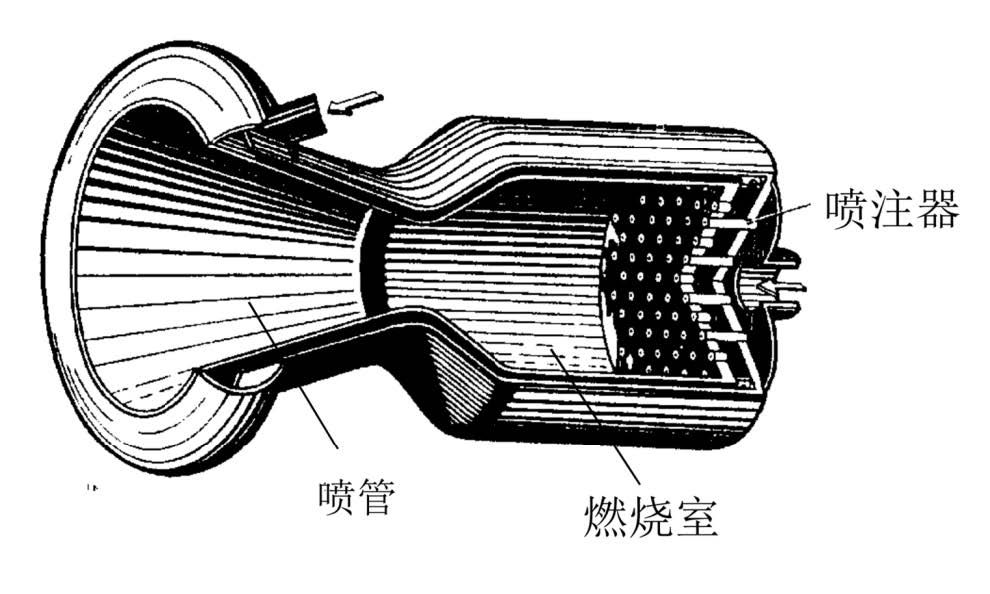
\includegraphics[width=\linewidth]{pic/推力室.jpg}
			\vspace*{-3em}
			\caption{推力室总体示意图}
			\label{推力室}
		\end{minipage}
		\begin{minipage}{0.45\linewidth}
			\centering
			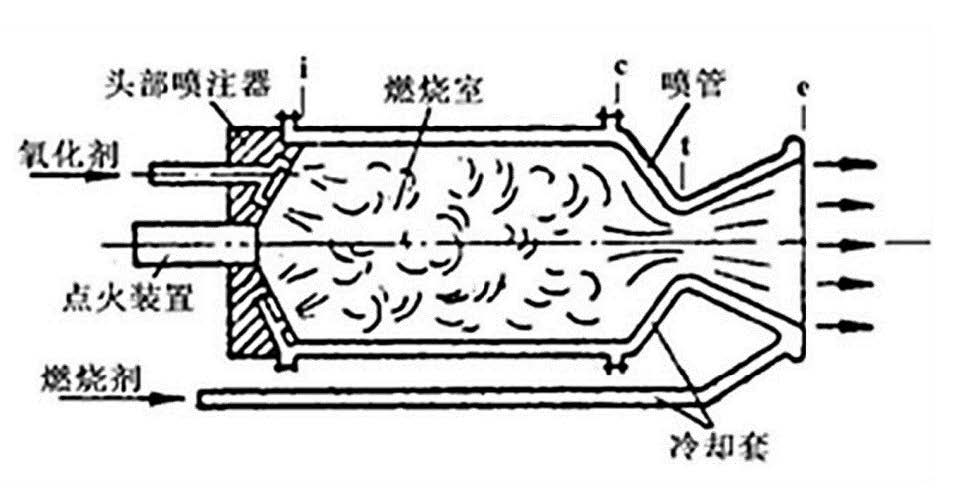
\includegraphics[width=\linewidth]{pic/推力室2.jpg}
			\vspace*{-2.8em}
			\caption{推力室内部示意图}
			\label{推力室2}
		\end{minipage}
	\end{figure}
	\vspace*{-1em}
	\item \textbf{工作过程} \hspace*{1em} 液体推进剂以\blue[规定的流量]和\blue[混合比]通过喷注器\blue[喷入燃烧室],在燃烧室内经过\blue[雾化、蒸发、混合和燃烧]等过程,产生的\blue[高温、高压燃气]在喷管内膨胀加速,以\blue[超声速]排出,从而产生推力。
	\item \textbf{特点} \hspace*{1em} \red[高温、高压环境],$3000\, \sim \, 4000 \degree\text{C}$,可以达到20$\,$MPa;\\
	\hspace*{3.5em}\red[化学反应速度很快,燃烧前准备过程决定燃烧速度]
\end{enumerate}

\sssection[推进剂供应系统]


\section{液体推进剂}
\subsection{液体推进剂分类及性能要求}
液体推进剂是翼液体状态进入推力室的推进剂,包括氧化剂和燃料以及单组元推进剂;可以是单质、化合物或混合物,是液体火箭发动机的能源和工质源,其质量占运载火箭起飞质量的70\% $\, \sim \,$90\%,直接影响着运载火箭和发动机的性能及制造费用。
\vspace*{0.5em}

\sssection[液体推进剂的分类]

\noindent \textbf{\underline{按进入推力室的基本组元数目分类}}
\vspace*{-0.5em}
\begin{enumerate}[\hspace*{1.5em} (1)  ]
	\item 单组元\\
	通过自身分解或燃烧能迅速产生高温高压的气体。\vspace*{-0.8em}
	\begin{enumerate}
		\item 在分子中同时含有可燃元素和燃烧所必需的氧的化合物,如:\underline{硝基甲烷、硝酸甲酯、过氧化氢} \vspace*{-0.5em}
		\item 在常压下互不产生化学反应的安定混合物,如:\underline{过氧化氢—甲醇}\vspace*{-0.5em}
		\item 在分解时能放出大量热量和气态产物的吸热化合物,如\underline{无水肼、甲基肼}\vspace*{-0.5em}
	\end{enumerate}
	单组元的特点:绝大多数单组元推进系统\blue[结构简单]、\blue[使用方便]、\blue[性能比较低]等\\
	单组元的应用:火箭发动机系统中的辅助能源,如涡轮泵燃气发生器、姿轨控制流
	
	\item 双组元\\
	由液体\red[燃烧剂]和\red[氧化剂]两种组员组成,工作时它们被分别从各自的贮箱和输送管路送入推力室。\vspace*{-0.8em}
	\begin{enumerate}
		\item 氧化剂:氧化力强的物质,如\underline{液氧、液氟、硝酸}等\vspace*{-0.5em}
		\item 燃烧剂(燃料):含氢量大、燃烧热值比较高的物质,如\underline{液氢、肼类、碳氢化合物}等\vspace*{-0.5em}
	\end{enumerate}
	双组元的特点:来源广泛、释放的能量较高\\
	双组元应用:液体火箭发动机绝大多数采用双组元推进剂
	
	\item 多组元
	由多于两组元组成的推进剂,常常指\dy[三组元]{SZY}。\vspace*{-0.8em}
	\begin{enumerate}
		\item 多于三组元的液体推进剂,理论上\red[能量不会进一步的增加]。\vspace*{-0.5em}
		\item 三组元足以能方便地把任何需要的化学元素组合起来。\vspace*{-0.5em}
	\end{enumerate}
	
	\item 三组元\vspace*{-0.8em}
	\begin{enumerate}
		\item 把轻金属(如锂、铍或铍的氢化物)同液氟、液氧或臭氧燃烧产生的高温与能够降低燃烧产物平均分子量的氢结合起来,提高比冲;\vspace*{-0.5em}
		\item 液氢、液氧和煤油 :在下面级工作时,常以氧为氧化剂、煤油为燃料并加入少量液氢燃料;\vspace*{-0.5em}
		\item 双燃料双膨胀:高压的内燃室中燃烧液氧、碳氢化合物;低压的外燃室燃烧液氧、液氢,带来起飞时高推力、小面积 比和高空的低推力、高面积比的优点。
	\end{enumerate}
\end{enumerate}

\noindent \textbf{\underline{按液体推进剂的贮存性能分类}}

\defination[地面可贮存推进剂]
{
	\dy[地面可贮存推进剂]{DMKZCTJJ} \quad 在\blue[相当宽的温度和压强范围]内、 在地面环境下能在贮箱内贮存一年或更长时间,不需外加能源加热熔化或冷却液化就能保持为液态又不变质的推进剂。多为硝基氧化剂、肼类、胺类和烃类燃料。
}
\noindent 具备条件:
\begin{enumerate}[\hspace*{1.5em}(1)  ]
	\item 临界温度不低于地面环境的最高温度\vspace*{-0.5em}
	\item 在323 K时的蒸气压不应大于2 MPa\vspace*{-0.5em}
	\item 在贮存期内,本身不分解变质、产生沉淀或放出气体\vspace*{-0.5em}
	\item 对与液体推进剂接触的部件不产生腐蚀。
\end{enumerate}

\defination[空间可贮存推进剂]
{
	\dy[空间可贮存推进剂]{KJKZCTJJ} \quad 在地面环境下不能贮存或难以贮存,但在空间环境下可以贮存的推进剂。其特点为其沸点低于空间环境温度,但高于200 K。
}

\noindent 空间不可贮存推进剂
\vspace*{-0.8em}
\begin{enumerate}[\hspace*{1.5em} (1) ]
	\item 低温推进剂\\
	定义:环境温度下是气体,沸点低于200 K,临界温度低于223 K,只有在低温才能保持为液态。\\
	特点:能量较高,使用不方便,有些价格昂贵;需要绝热措施和排气系统;液氧、液氢、液氟、二氟化氧及其某些混合物。\vspace*{-0.5em}
	
	\item 化学不稳定推进剂\\
	化学性质不稳定而只能在短期内使用。如,\underline{过氧化氢、叠氮化肼}。
\end{enumerate}

\noindent \textbf{\underline{按推进剂能量高低分类}}

\noindent 分类方法:采用一定的发动机工况(室压7 MPa、喷管出口截面出燃气压强0.1 MPa)时,发动机比冲大小。\vspace*{-0.5em}
\begin{enumerate}[\hspace*{1.5em} (1)  ]
	\item \dy[高能推进剂]{GNTJJ} \quad 比冲一般大于3000 m/s \vspace*{-0.5em}
	\item \dy[中能推进剂]{ZNTJJ} \quad 比冲在2500$\, \sim \,$3000 m/s之间 \vspace*{-0.5em}
	\item \dy[低能推进剂]{DNTJJ} \quad 比冲小于2500 m/s
\end{enumerate}

\noindent \textbf{\underline{按发动机用途分类}}

\dy[主推进剂]{ZTJJ}主要用于火箭、导弹等的主发动机

\dy[辅助推进剂]{FZTJJ}主要用于辅助发动机和发动机辅助系统

\vspace*{0.5em}

\noindent \textbf{\underline{按推进剂的自燃性质分类}}

\dy[自燃推进剂]{ZRTJJ}\quad 经简单混合后能自燃的推进剂

\dy[非自燃推进剂]{FZRTJJ} \quad 燃烧必需依靠外部提供能量,即需要点火装置


\sssection[发动机对液体推进剂对要求]

对液体推进剂对要求主要包括\underline{性能要求、使用要求、经济性要求}。
\vspace*{0.5em}

\noindent \textbf{\underline{性能要求}}\vspace*{-0.5em}
\begin{enumerate}[\hspace*{1.5em} (1) ]
	\item 高的比冲和高的密度\vspace*{-0.5em}
	\item 具有较高的热值\vspace*{-0.5em}
	\item 燃烧产物温度要高、分子量要低、燃烧产物不易解离、没有液态或固态产物存在
\end{enumerate}

\noindent \textbf{\underline{使用要求}}

要求液体推进剂的液态温度范围较宽、化学性质稳定且毒性小,对人员、设备和环境对污染小等。使用性能具体表现在
\vspace*{-0.5em}
\begin{enumerate}[\hspace*{1.5em} (1) ]
	\item \red[具有良好的运输型和输送性]\\
	粘度小其粘度随温度的变化率小;饱和蒸汽压小;推进剂中溶解的气体量少;所含悬浮颗粒物、粘性物质少
	\vspace*{-0.5em}
	
	\item \red[具有良好的点火和燃烧特性]\\
	着火延迟期(自燃推进剂)和点火延迟期不大于30 ms。
	
	\item \red[具有良好的冷却性能]
	\vspace*{-0.5em}
	
	\item \red[贮存稳定性好]\\
	与贮存材料相容性好;对空气和空气中的湿度不过于敏感;能经受环境温度的急剧变化。
	
	\item \red[具有良好的安全性能]\\
	热爆炸和热分解温度要搞;对机械冲击和突然压缩(水击)不敏感;无毒或低毒,燃烧产物对人和环境对毒害作用小。
\end{enumerate}

\noindent \textbf{\underline{经济型要求}}

原材料来源广泛、生产工艺简单、价格便宜。
\vspace*{0.5em}

\sssection[选择推进剂的原则]
\vspace*{-0.8em}
\begin{enumerate}[\hspace*{1.5em} (1)  ]
	\item 单位质量所释放的能量高、燃气的平均分子量要低 $\longrightarrow$ 确保高比冲\vspace*{-0.5em}
	\item 易于点火、燃烧稳定\vspace*{-0.5em}
	\item 密度大$\longrightarrow$较小推进剂贮箱和供应系统的尺寸和重量\vspace*{-0.5em}
	\item 高比热容、高热导率和高临界温度的最佳组合$\longrightarrow$可用作推力室的有效冷却剂\vspace*{-0.5em}
	\item 更低的饱和蒸汽压$\longrightarrow$利于泵的工作和设计\vspace*{-0.5em}
	\item 低冰点、高沸点 $\longrightarrow$ 发动机工作温度宽\vspace*{-0.5em}
	\item 无腐蚀性、毒性小 $\longrightarrow$ 与材料相容性好,对环境污染小\vspace*{-0.5em}
	\item 具有良好对可贮存性\vspace*{-0.5em}
	\item 低粘度 $\longrightarrow$ 易输送,通过供应系统和喷注器的压降小\vspace*{-0.5em}
	\item 高的热和冲击稳定性 $\longrightarrow$ 危险性小\vspace*{-0.5em}
	\item 低成本
\end{enumerate}
\vspace*{0.5em}

\subsection{液体推进剂物理化学参数}


\section{液体火箭发动机系统及工作}
\subsection{挤压式推进剂供应系统}
\noindent \textbf{\underline{推进剂供应系统}}

\blue[功能]\quad 将贮箱中的推进剂按照要求的流量和压强输送到推力室中。

\blue[分类]\quad 按其工作的方式,可分为挤压式和泵压式两大类。
\vspace*{0.5em}

\clearpage
\begin{minipage}{0.5\linewidth}
	\noindent \textbf{\underline{挤压式推进剂供应系统}}
	
	\blue[原理]\quad 利用高压气体将液体推进剂挤压出来输送到推力室;
	
	\blue[优缺点]\quad 简单、可靠;较高压强下结构比较笨重;
	
	\blue[适用性]\quad 小推力、工作时间较短;
	\vspace*{0.8em}
	
	\blue[组成]  \quad 
	$
	\begin{cases}
		\, \mbox{推进剂贮箱}\\
		\, \mbox{用来建立供应压强的气源}\\
		\, \mbox{各种功能的阀门}\\
		\, \mbox{参数调节或校准元件}\\
		\, \mbox{导管和其他附件}
	\end{cases}
	$
\end{minipage}
\begin{minipage}{0.5\linewidth}
	\centering
	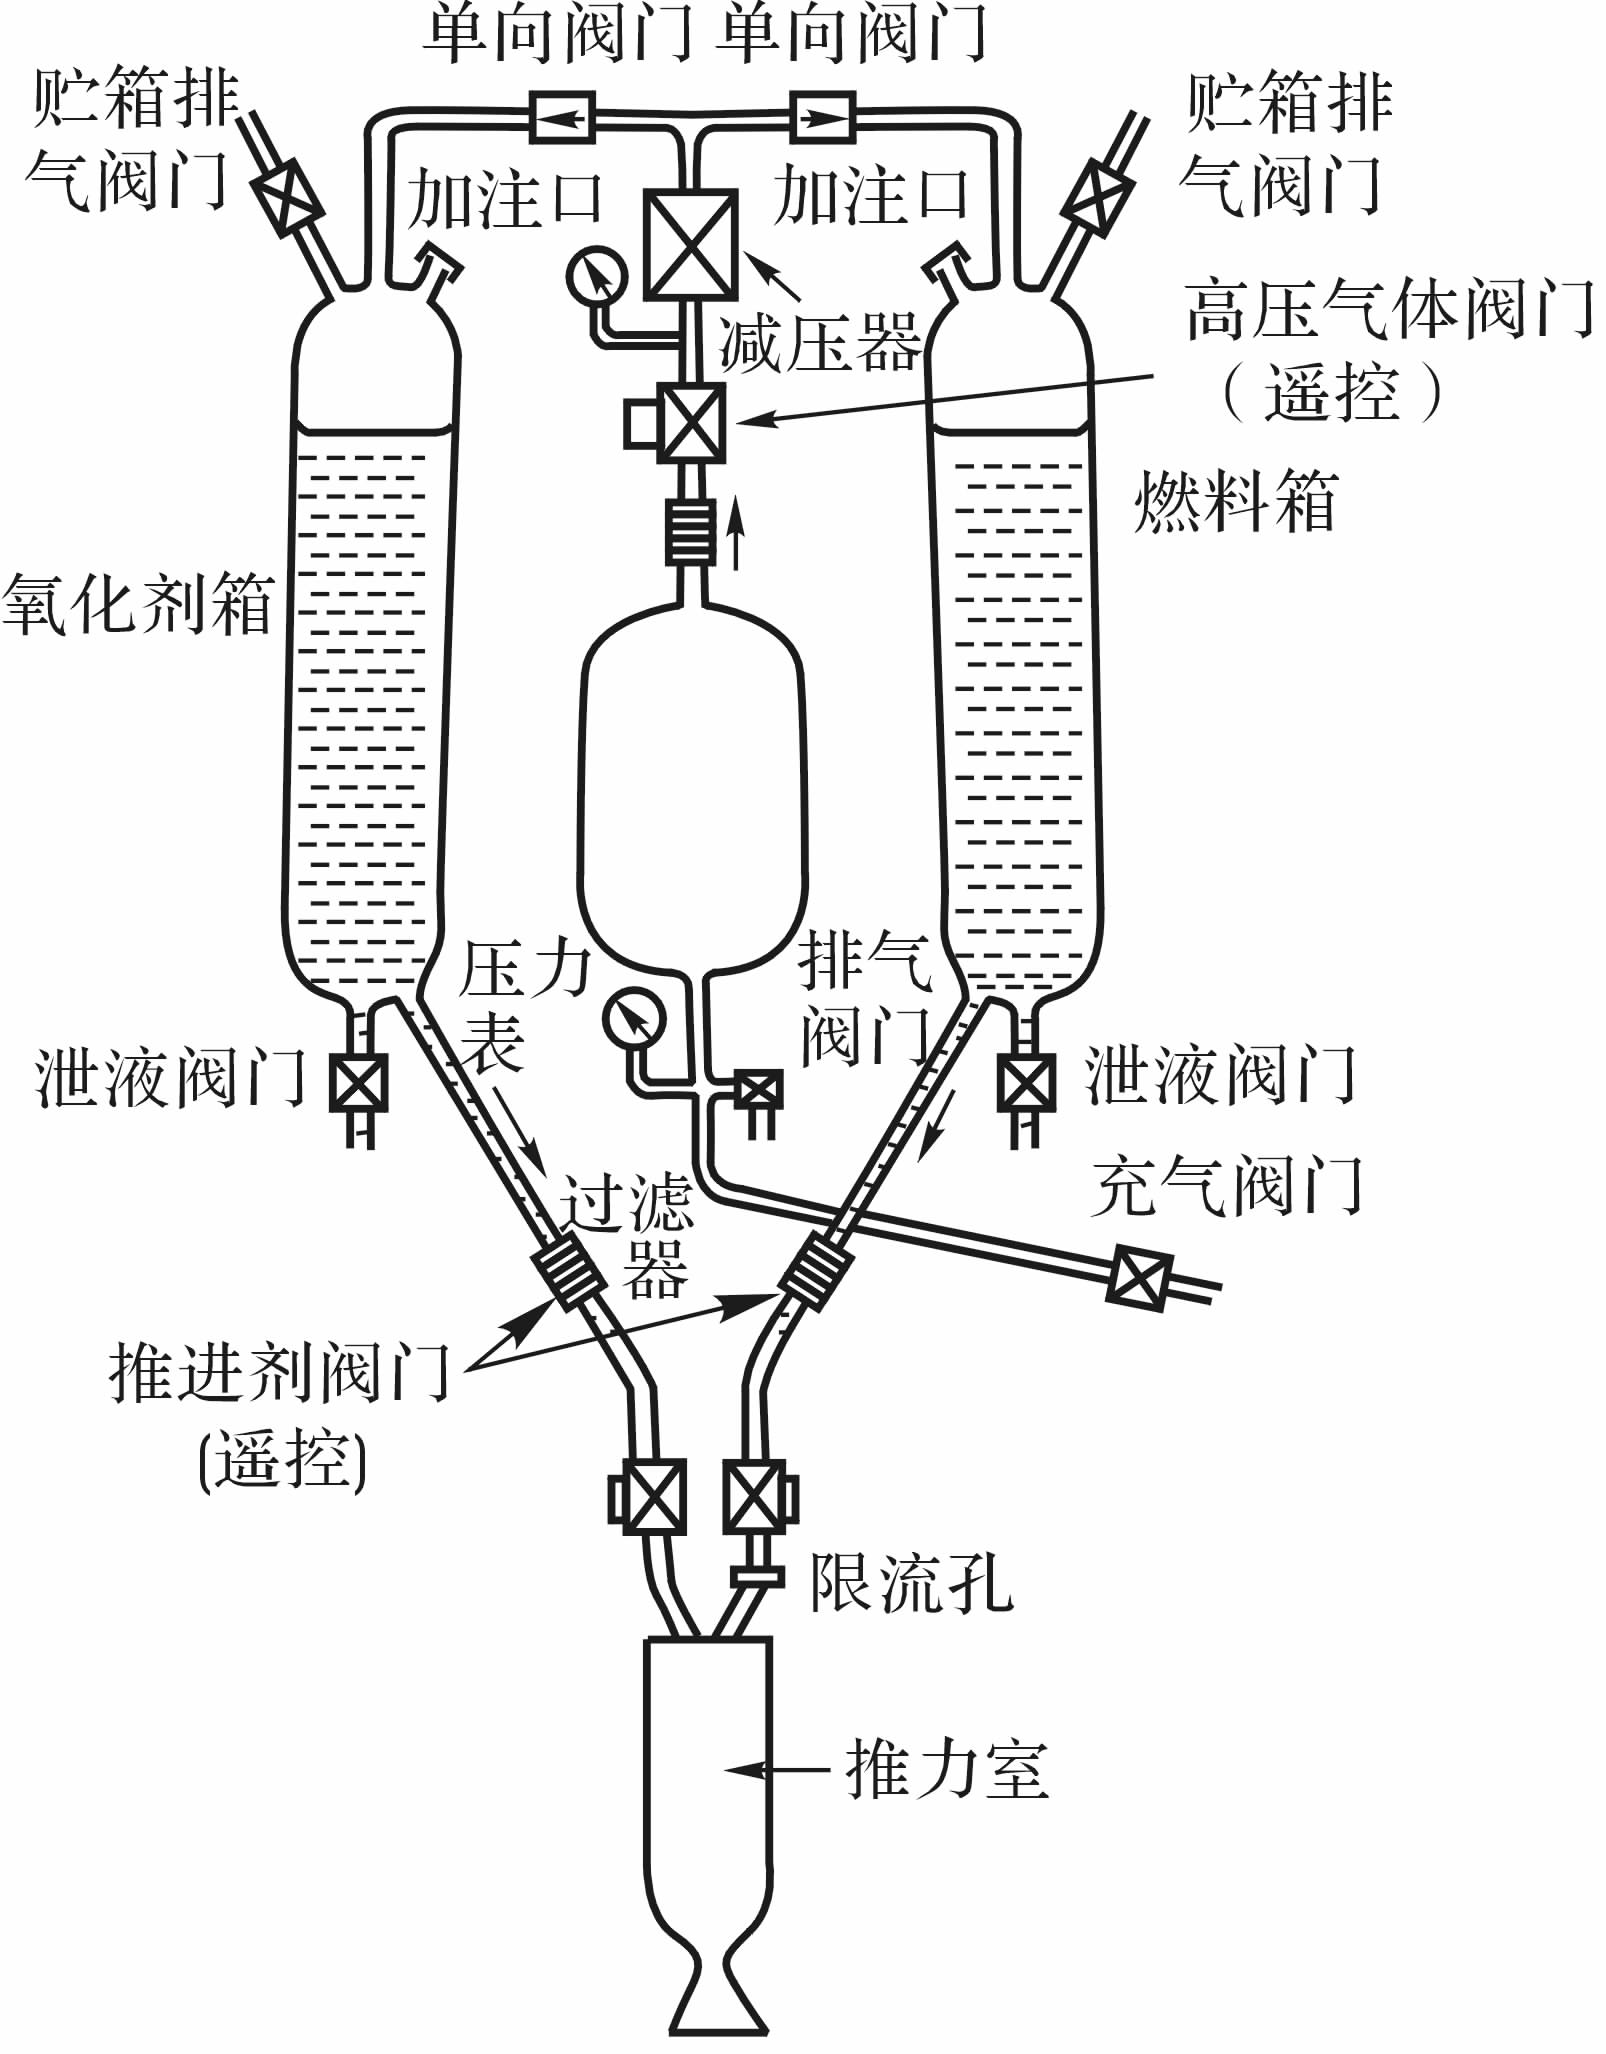
\includegraphics[width=0.8\linewidth]{pic/气压.png}
	\captionof{figure}{气体挤压式推进剂供应系统}
\end{minipage}


\vspace*{0.8em}
\noindent
\begin{minipage}{0.6\linewidth}
	\sssection[挤压式供应系统分类]
	
	\blue[对挤压工质的要求]\quad 与推进剂有良好的\red[相容性] ;最小的分子量具有适当的温度,且热稳定性要好。
	
	挤压气源是来自高压气瓶,瓶内压强约为20$\, \sim \,$35 MPa ,通过降压方式到工作压强。按照降压方式,又分为减压器降压式和直接膨胀降压式。
	\vspace*{0.8em}
	
	\sssection[冷气体挤压]
	\vspace*{-0.8em}
	\begin{enumerate}[\hspace*{1.5em} (1) ]
		\item \textbf{气瓶式(或贮气式)冷气挤压}\\
		\blue[常用挤压气体] \quad 空气、氮气和氦气。对于低温推进剂,空气和氮气遇冷后会发生凝结,应选用氦气。\vspace*{-0.5em}
		
		\item \textbf{蒸发系统汽化式}\\
		挤压气源是利用液体的汽化而得到。\\[0.5em]
		按照使用液体的来源,分为推进剂蒸发系统和非推进剂蒸发系统,即将容易气化的推进剂组元或非推进剂液体通过换热器加热、气化后去挤压贮箱中的推进剂。
		\begin{equation*}
			\begin{cases}
				\, \mbox{\blue[推进剂蒸发系统]}\quad \mbox{仅适用于热稳定的低沸点推进剂,如氢;(注:也适用泵式发动机)}\\
				\, \mbox{\blue[非推进剂蒸发系统]} \quad \mbox{主要是惰性气体蒸发系统,如液氮、液氦}
			\end{cases}
		\end{equation*}
	\end{enumerate}
\end{minipage}
\begin{minipage}{0.4\linewidth}
	\centering
	\vspace*{-4em}
	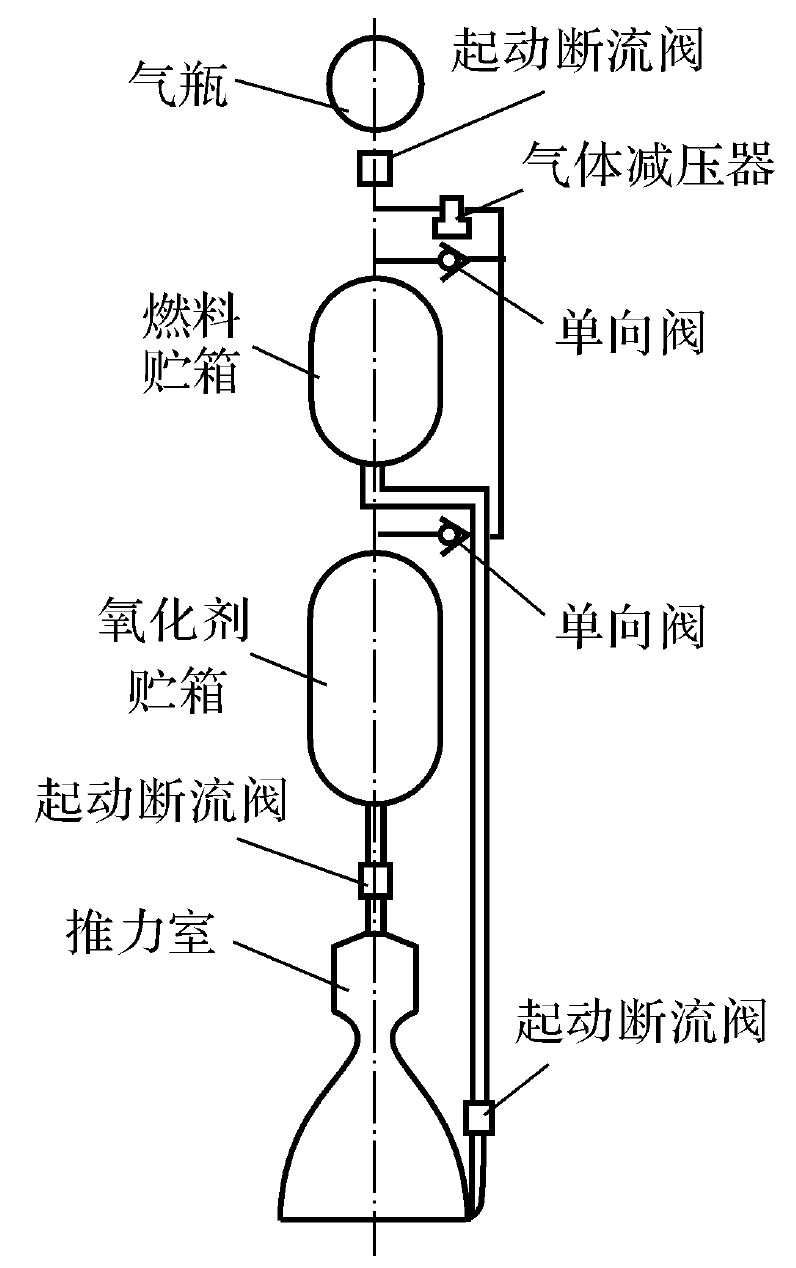
\includegraphics[width=0.8\linewidth]{pic/气瓶挤压.png}
	\vspace*{-1em}
	\captionof{figure}{气瓶式挤压式推进剂供应系统}
\end{minipage}

\vspace*{1em}
\sssection[热气体挤压]

\blue[适用范围] \quad 不能应用于低温推进剂:产物中的水会凝结吸热,会提高低温推进剂的温度。
\vspace*{0.5em}

\blue[分类]\quad 按产生热挤压气体的途径分类:
$
\begin{cases}
	\, \mbox{燃气发生器式}\\
	\, \mbox{化学反应式}
\end{cases}
$

\begin{enumerate}[\hspace*{1.5em} (1) ]
	\item \textbf{燃气发生器}\\
	按使用推进剂分类:
	\vspace*{-0.5em}
	\begin{enumerate}
		\item 固体燃气发生器\\
		基本组成\quad 固体推进剂燃气发生器(壳体、药柱、点火器)、过滤器和燃气调节装置及冷却热燃气的装置(不是必须)等。
		\begin{table}[!htb]
			\centering
			\setlength{\tabcolsep}{14mm}{
			\begin{tabular}{cl}
				\toprule
				固体燃气发生器类型 & 基本原理\\
				\midrule
				\makecell[c]{无冷却的\\固体燃气发生器} & \makecell[l]{固体燃气发生器产生燃气;\\过滤器过滤燃气;\\调节器排出多余燃气。}\\
				\hline
				 \makecell[c]{使用固体冷却剂的\\燃气发生器
} &\makecell[l]{推进剂:硝酸铵基;  冷却剂:粒状的草酸。 \\热燃气通过固体冷却剂冷却升华\\或分解产生附加的挤压气体($\text{CO}_2, \text{H}_2\text{O}, \text{CO}$)。}\\
				 \hline
				 \makecell[c]{使用叠氮化物冷却的\\燃气发生器} & \makecell[l]{热燃气通过叠氮化物冷却层被冷却,\\叠氮化物分解并产生氮气;\\但燃气中含有金属粒子,要用旋转分离除去。\\能提供较纯的氮气。
				 }\\
				 \hline
				 \makecell[c]{使用燃气发生器\\加热的氮气系统
} & \makecell[l]{固体燃气发生器安装在氦气瓶内,\\提供热量和 附加的挤压气体。
}\\
				\bottomrule
			\end{tabular}
		}
		\end{table}
	
	\begin{figure}[!htb]
		\begin{minipage}{0.25\linewidth}
			\centering
			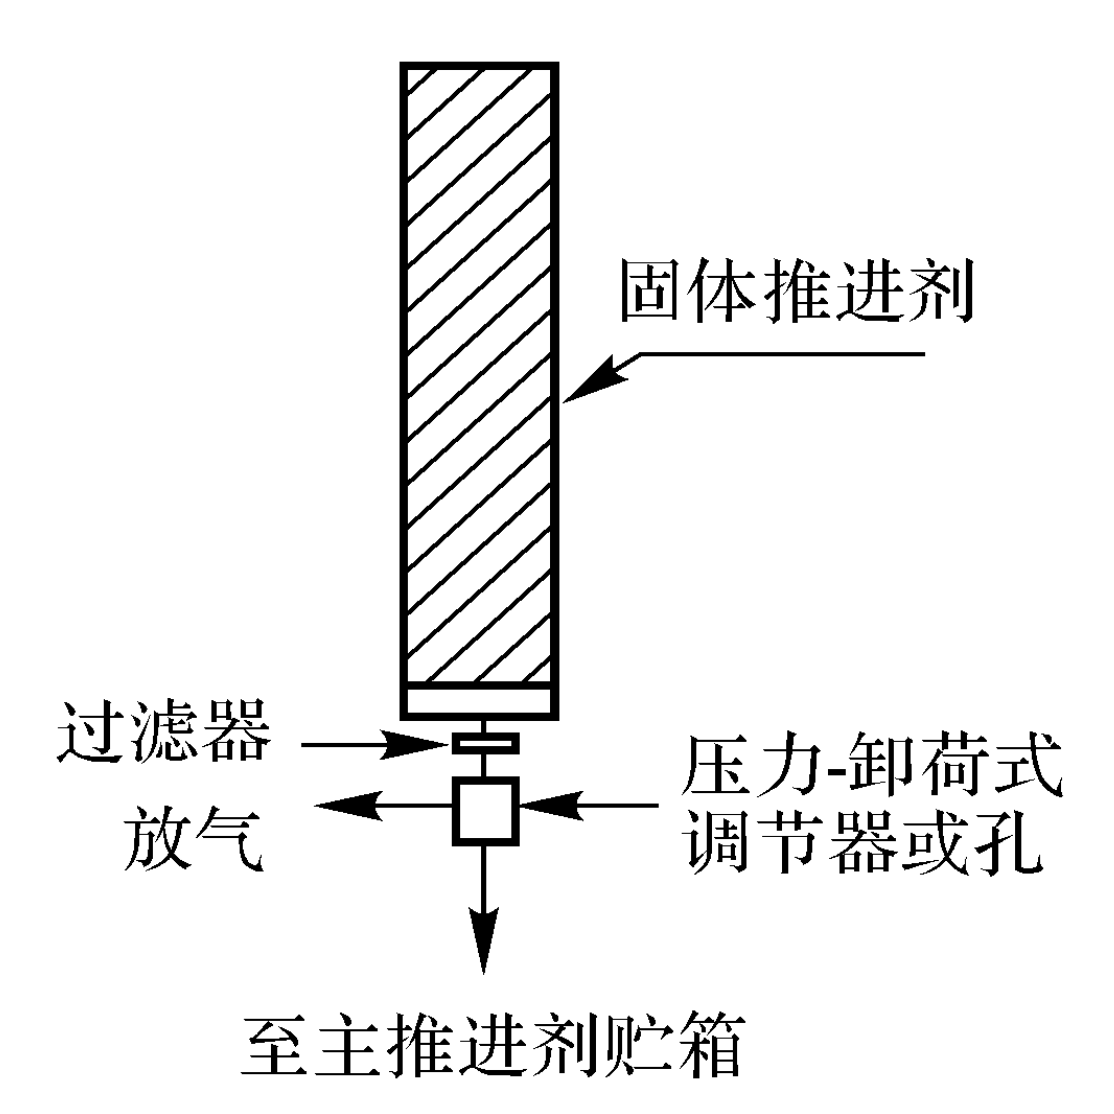
\includegraphics[width=\linewidth]{pic/固体1.png}
		\end{minipage}
		\begin{minipage}{0.25\linewidth}
			\centering
			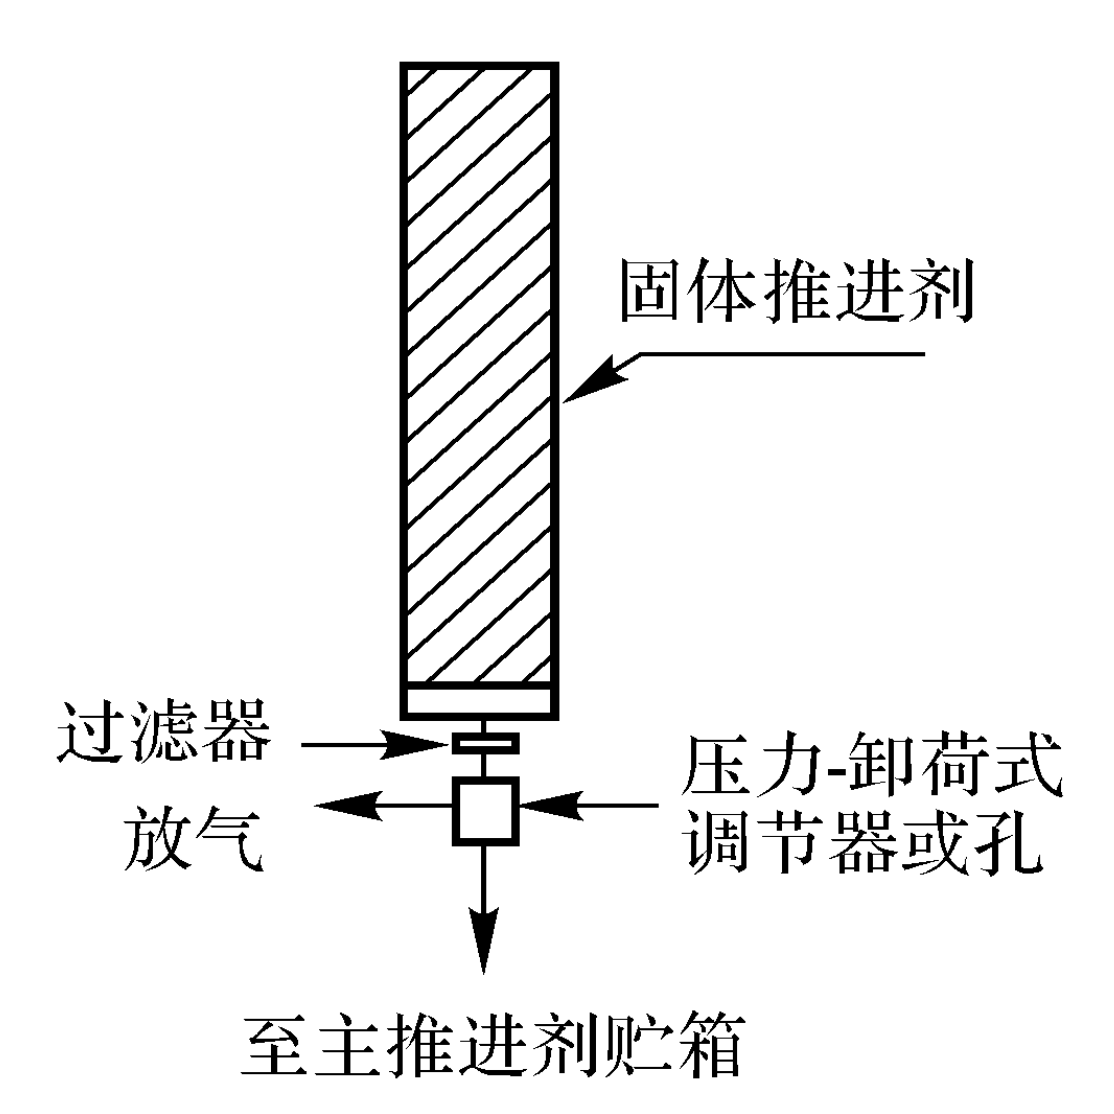
\includegraphics[width=\linewidth]{pic/固体1.png}
		\end{minipage}
		\begin{minipage}{0.25\linewidth}
			\centering
			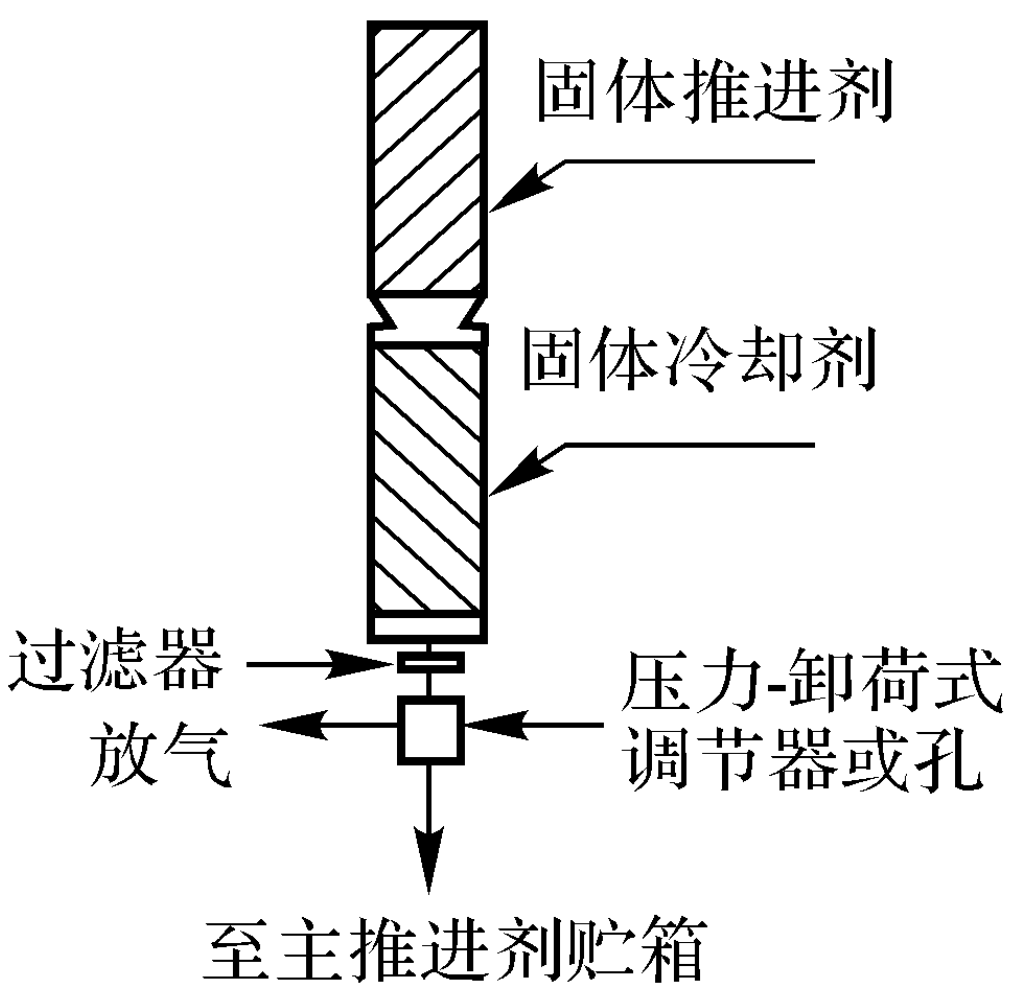
\includegraphics[width=\linewidth]{pic/固体3.png}
		\end{minipage}
		\begin{minipage}{0.20\linewidth}
			\centering
			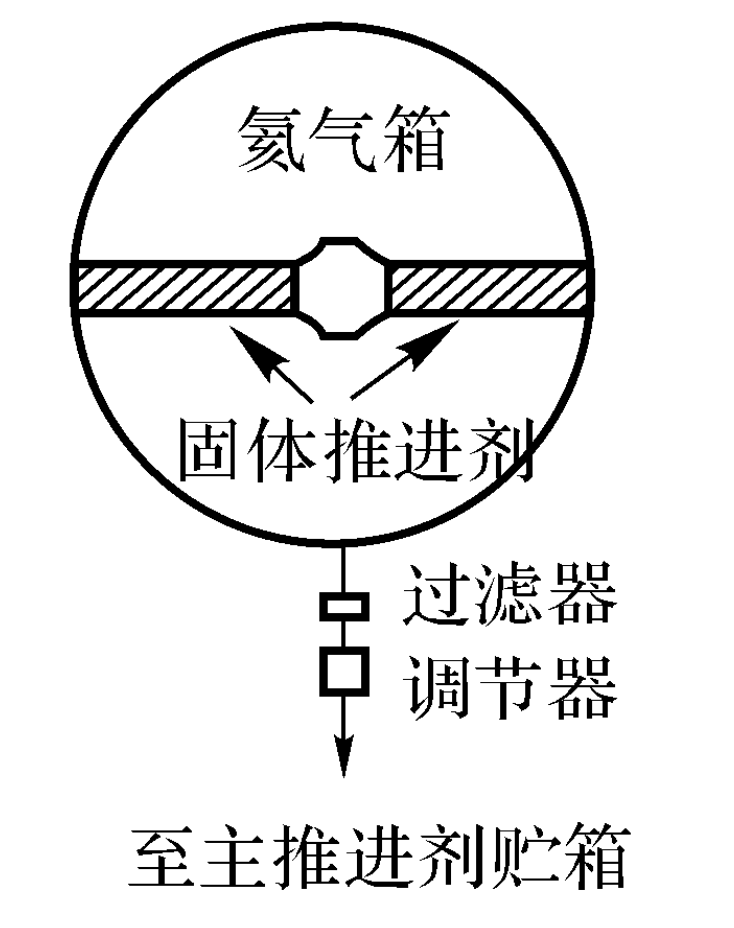
\includegraphics[width=\linewidth]{pic/固体4.png}
		\end{minipage}
	\caption{四种固体燃气发生器类型}
	\end{figure}
	
	\item 液体燃气发生器
	\begin{table}[!htb]
		\centering
		\setlength{\tabcolsep}{10mm}{
			\begin{tabular}{cl}
				\toprule
				液体燃气发生器类型 & 基本原理\\
				\midrule
				\makecell[c]{具有喷注冷却的\\单燃气发生器} & \makecell[l]{单组元$+$不反应的冷却剂, 产生低温燃气;\\
				双组元,使混合比远远偏离化学当量比,产生低温燃气。}\\
				\hline
				\makecell[c]{具有单个燃气\\发生器的氦气系统
} &\makecell[l]{燃气发生器通过换热器加热氦气,\\用热氦气其挤压 氧化剂贮箱;
\\燃气挤压主燃料贮箱。}\\
				\hline
				\makecell[c]{具有喷注冷却的\\两个双组元燃气发生器} & \makecell[l]{用氦气挤压两个辅助推进剂贮箱,供应燃气发生器;
\\富燃燃气发生器产生的燃气挤压主燃料贮箱;\\
富氧的燃气发生器产生的燃气挤压主氧化剂贮箱。}\\
				\bottomrule
			\end{tabular}
		}
	\end{table}
	
	典型的双组元液体燃气发生器式挤压系统如图\ref{双组元}所示。
	\end{enumerate}
	
	\begin{figure}[!htb]
		\centering
		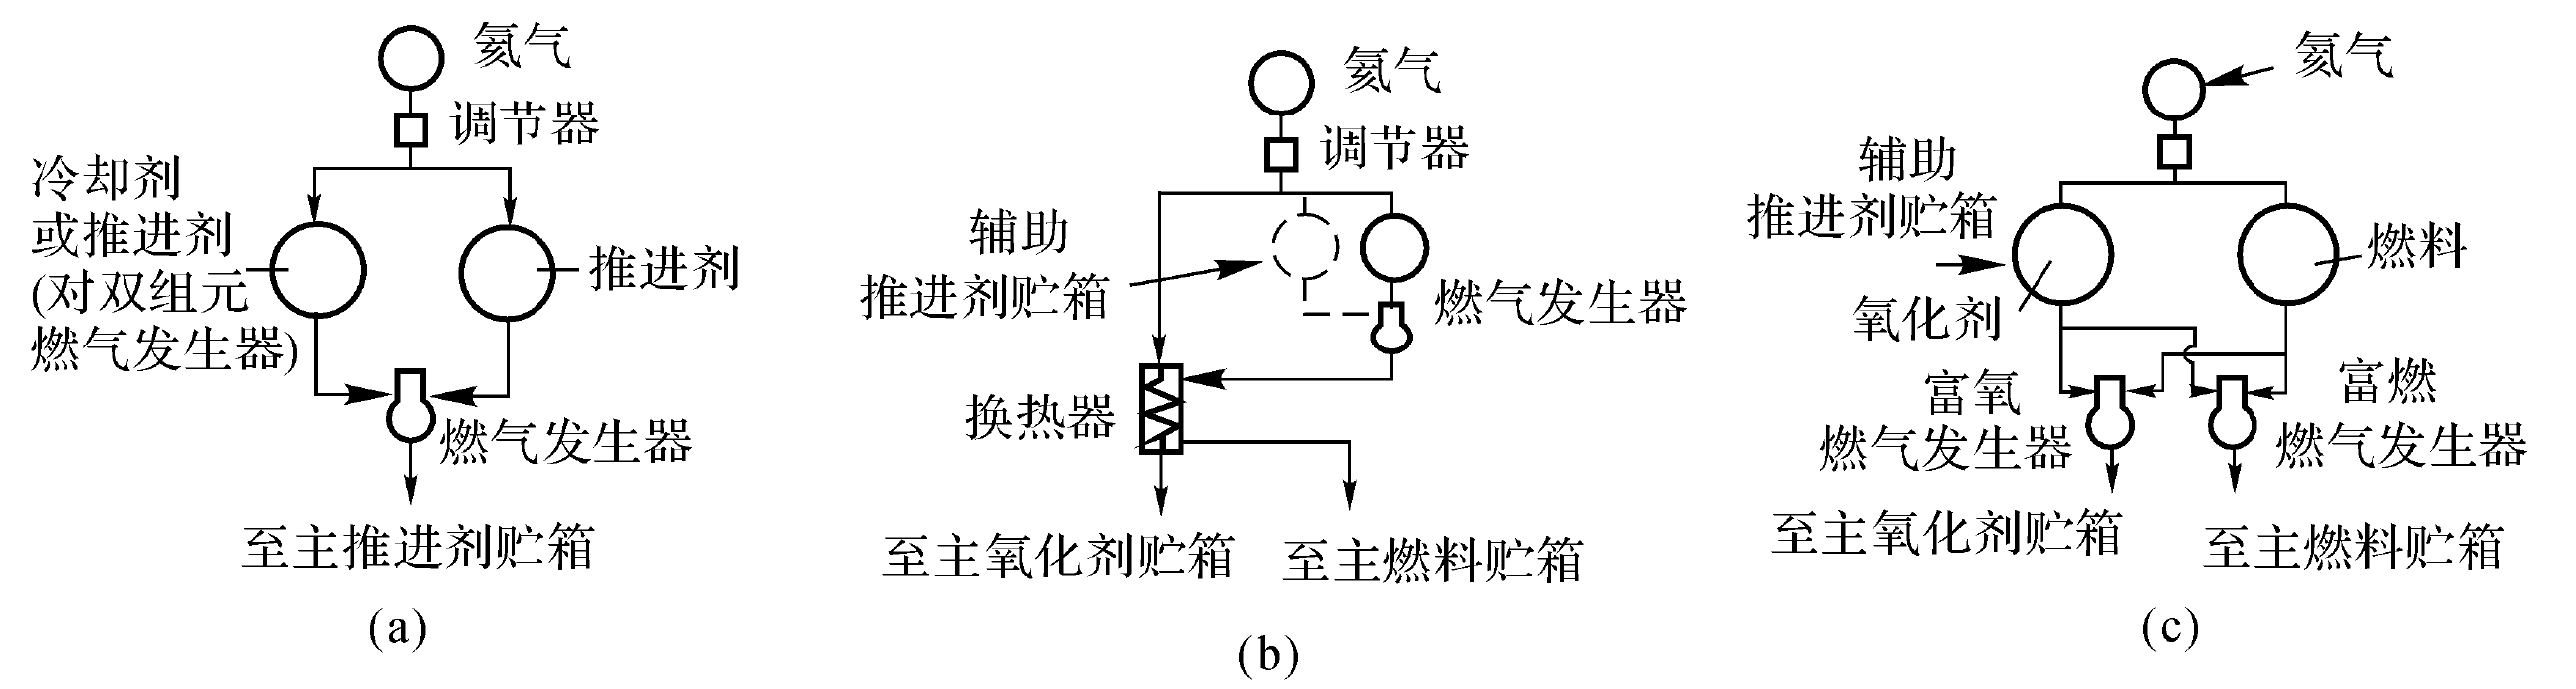
\includegraphics[width=0.9\linewidth]{pic/液体.png}
		\caption{三种液体燃气发生器类型}
	\end{figure}
	
	\begin{figure}[!htb]
		\centering
		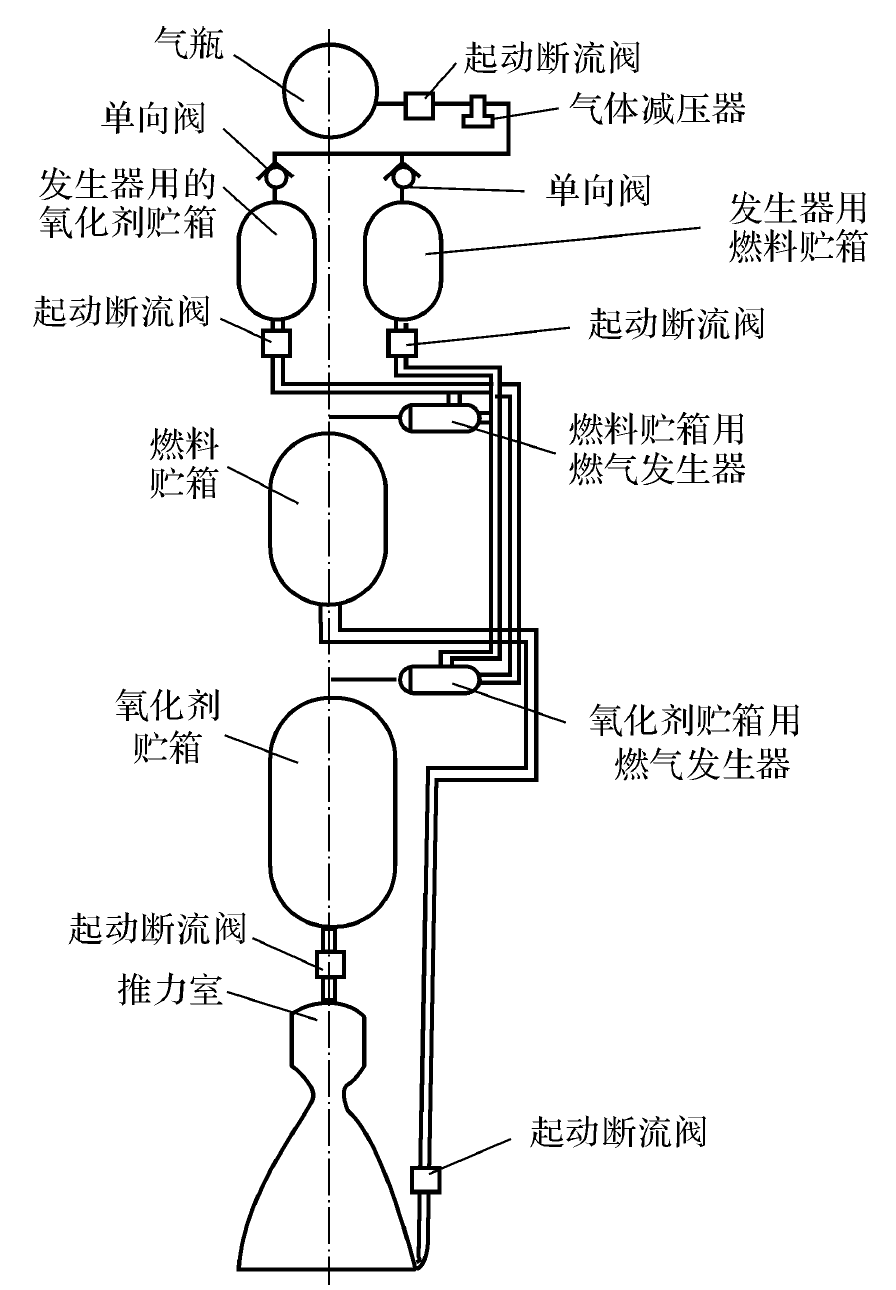
\includegraphics[width=0.35\linewidth]{pic/双组元液体.png}
		\caption{双组元液体燃气发生器式挤压系统}
		\label{双组元}
	\end{figure}
	
	\item \textbf{化学反应式}\\
	在贮箱中直接发生化学反应,即将少量燃料喷注到氧化剂贮箱中,或
将少量氧化剂喷注到燃料贮箱中,发生化学反应,从而产生挤压气体。
有两种类型:
	\vspace*{-0.5em}
	\begin{itemize}
		\item \blue[双直接喷注式]\quad 两个辅助贮箱。
		\item \blue[串联直接喷注式]\quad 一个辅助贮箱;在系统安全、可靠性和 调节贮箱稳态压力等方面存在设计问题。
	\end{itemize}
	\begin{figure}[!htb]
		\centering
		\subfigure[双直接喷注式]{
		\begin{minipage}{0.4\linewidth}
			\centering
			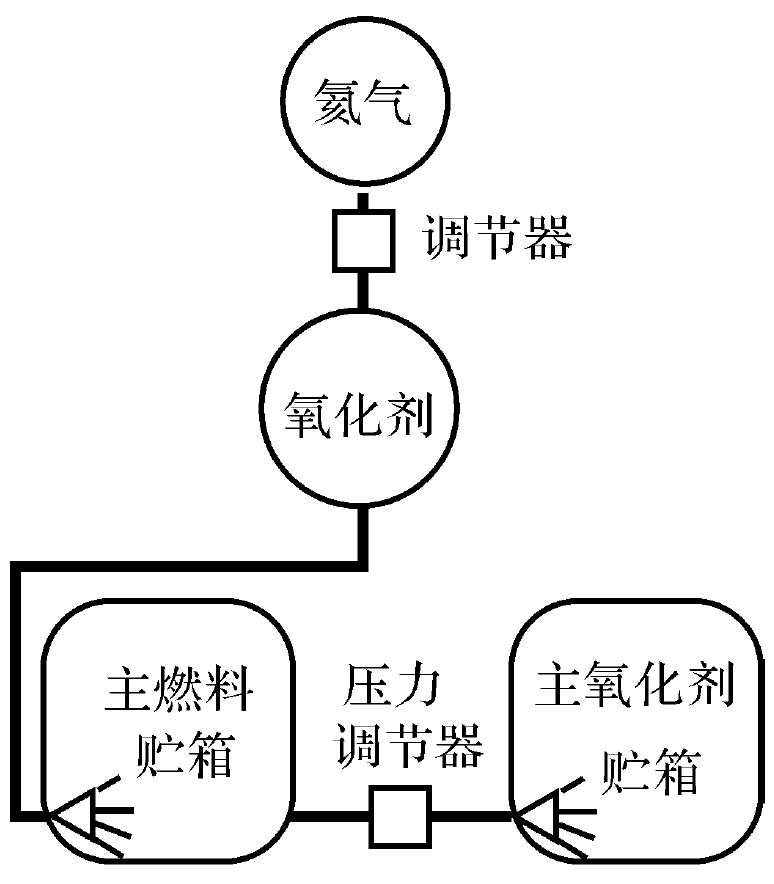
\includegraphics[width=0.5\linewidth]{pic/化学1.png}
			\vspace*{0.5em}
		\end{minipage}
		}
		\subfigure[串联直接喷注式]{
		\begin{minipage}{0.4\linewidth}
			\centering
			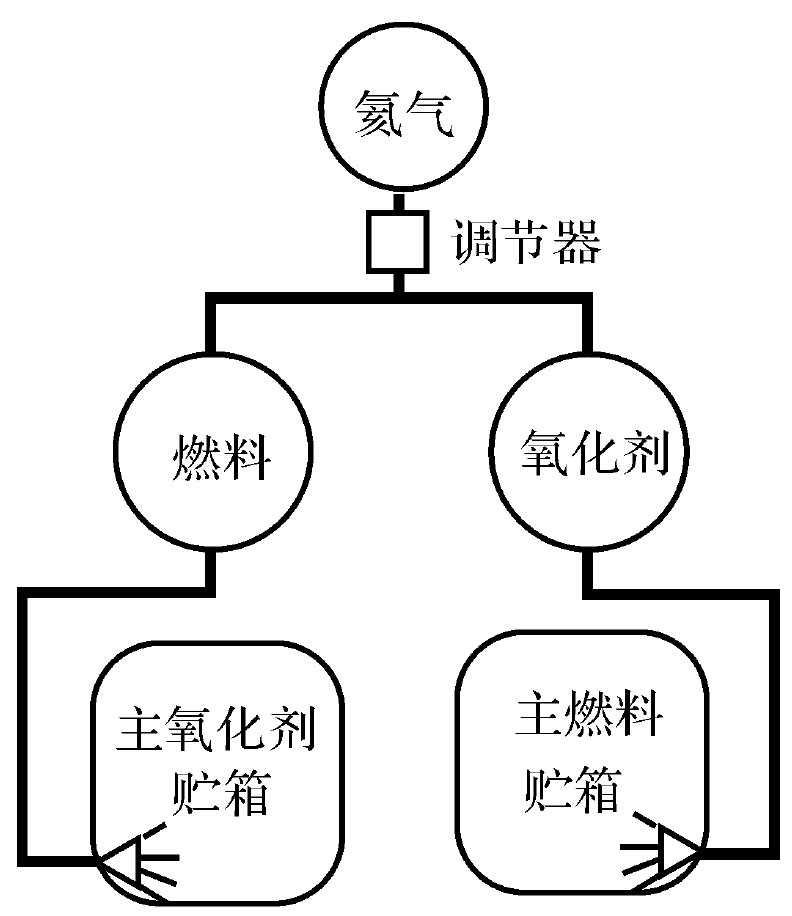
\includegraphics[width=0.5\linewidth]{pic/化学2.png}
			\vspace*{0.5em}
		\end{minipage}
	}
	\caption{化学反应式挤压系统}
	\vspace*{-2em}
	\end{figure}
\end{enumerate}

\sssection[各种挤压系统的对比]
\begin{table}[!htb]
	\centering
	\setlength{\tabcolsep}{2.5mm}{
	\begin{tabular}{m{0.1\textwidth}<{\centering} m{0.25\textwidth}<{\centering} m{0.25\textwidth}<{\centering} m{0.28\textwidth}<{\centering}}
		\toprule
		类别 & 气瓶贮气系统 & 液体蒸发系统 & 热气挤压系统 \\
		\midrule
		优点 & 结构简单,技术成熟 & 辅助气瓶和辅助贮箱尺寸小系统结构质量小 & 辅助气瓶和辅助贮箱尺寸小,系统结构质量小固体发生器系统结构简单\\
		\hline
		缺点 & 气瓶容积大,系统质量大 & 需要辅助气瓶、辅助贮箱和换热器,结构复杂 & 对液体发生器和在贮箱中直接化学反应的系统,结构复杂;固体发生器系统不能多次起动\\
		\hline
		适用范围 & 总冲量比较小的发动机 & 热稳定、低沸点的推进剂组元,若推进剂都不易汽化,可以选用液化气体 & 常温推进剂\\
		\bottomrule
	\end{tabular}
}
\end{table}

\noindent \textbf{\underline{挤压系统的选择}}

\par (1) \hspace*{0.5em}\red[任务和运载器的要求。]包括贮存性能、系统的起动和再起动以及压强和流量的精度等。
\par (2) \hspace*{0.5em}\red[挤压气体与推进剂、贮箱材料的相容性。] 包括化学惰性、过凝结和过溶解气体产物的防止以及适当的挤压物质温度。
\par (3) \hspace*{0.5em}\red[挤压式系统的可靠性。] 可靠性是在系统复杂性和失效模式的基础上估计的,应大力发展可靠性高的组件,包括燃气发生器、换热器和调节器等。
\par (4) \hspace*{0.5em}\red[成本。]
\par (5) \hspace*{0.5em}\red[挤压式系统的重量和尺寸。]

挤压系统的\blue[特点]:技术成熟,可靠性高;系统比较笨重。\blue[适用于]小推力或工作时间较短的火箭发动机。
\vspace*{0.5em}

\subsection{泵压式推进剂供应系统}

\begin{figure}[!htb]
	\centering
	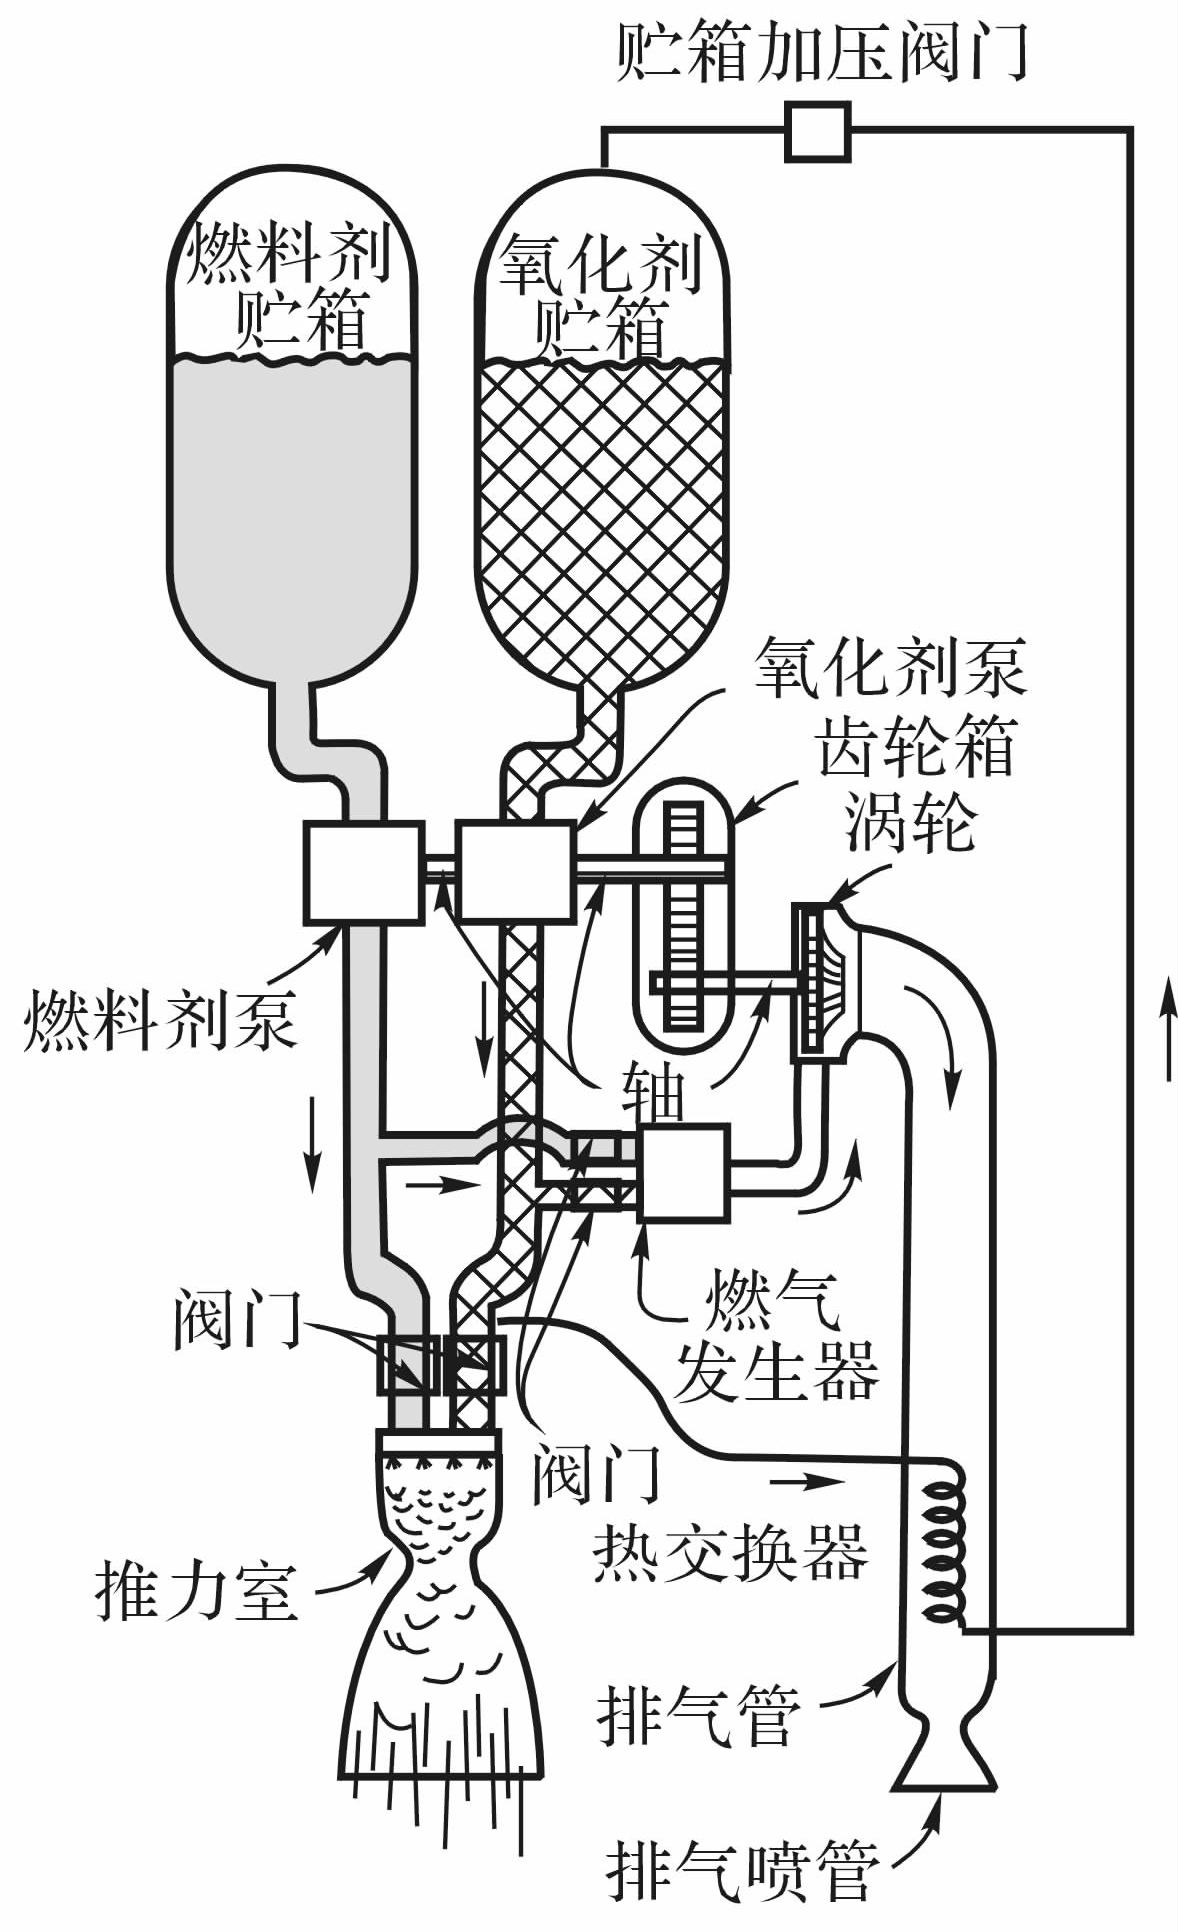
\includegraphics[width=0.3\linewidth]{pic/泵压.png}
	\caption{泵压式推进剂供应系统}
\end{figure}

\defination[泵压式供应系统]
{
	\blue[原理]\quad 利用涡轮泵将推进剂从贮箱中抽出、增压,输送至推力室;\\
	\hspace*{2em} \blue[关键部件]\quad 涡轮泵\\
	\hspace*{2em} \blue[特点]\quad 泵前推进剂是低压,贮箱结构质量可以较轻,一般$\le 0.5\,$MPa.\\
	\hspace*{2em} \blue[适用]\quad 工作时间长的大中型液体发动机。
}





















%第四章:功和能
\chapter{积分变换法}
\thispagestyle{empty}

\tdefination[积分变换]
把函数$f(t)$经过积分运算变换为另一类函数
\begin{align}
	F(\beta) = \int_a^b f(t)K(\beta, t) \, \d t
\end{align}
其中,
\begin{itemize}
	\item $\beta$为参变量,$K(\beta, t)$为一个确定的二元函数,称为\dy[积分变换的核]{JFBHDH}\vspace*{-0.5em}
	\item 不同的核与不同的积分区域,构成不同的积分变换\vspace*{-0.5em}
	\item 主要包括Fourier变换和Laplace变换
\end{itemize}

\section{Fourier变换}
\vspace{0.5em}
\ttheorem[Fourier变换]
\dy[Fourier变换]{FourierBH}
\begin{align}
	F(\omega) = \mathcal{F}\big[f(x)\big] = \int_{- \infty}^{+ \infty} f(x) \e^{- \i \omega x}\, \d x
\end{align}
\vspace*{-2em}

\dy[反演]{FY}
\begin{align}
	f(x) = \mathcal{F}^{-1} \big[F(\omega)\big] = \dfrac{1}{2 \pi} \int_{- \infty}^{+ \infty} F(\omega) \e^{\i \omega x}\, \d \omega
\end{align}

\warn[
Fourier变换的重要条件:\textbf{分段光滑}\footnote{\textbf{分段光滑}:一阶导数存在,且导函数只有第一类间断点。}、\textbf{绝对可积}$\displaystyle \int_{- \infty }^{+ \infty} \big|f(x)\big|\, \d x < + \infty$\vspace*{-0.5em}
{
\begin{enumerate}[\hspace*{2em} \textbf{推论} 1 \hspace*{2em}]
	\item $\displaystyle \int_{- \infty}^{+ \infty} f(x)\, \d x = \mbox{有限值}$
	\item $x \to \pm \infty, f(x) \to 0$
\end{enumerate}
}
]

\subsection{Fourier变换的理解}
Fourier变换从几何上看是将函数分解成无数个绕原点做圆周运动的向量,得到相位/半径 与频率的函数关系;本质上是分解成无数个不同频率、幅值和相位正弦函数。

物理上认为,$f(x)$为信号(原函数), $F(\omega)$为频谱(像函数),对$f(x)$进行Fourier变换,实际上是由信号得到频谱的过程(从时域到频域),称为\dy[Fourier分析]{FourierFX}。

对于Fourier变换的进一步理解,如图\ref{Fourier变换的理解图}.

\begin{figure}[!htb]
	\centering
	\begin{tikzpicture}
		\node (A) [draw, inner sep = 5pt]{\makecell[c]{周期函数可以表示为不同频率、\\幅值和相位的正弦函数的叠加}};
		\node (B) [draw, inner sep = 5pt, below of = A, node distance = 3.5cm]{\makecell[c]{当函数的周期较小时,正弦函数的频率\\是稀疏的,因此叠加体现为无穷级数}};
		\node (B1) [draw, inner sep = 5pt, right of = B, node distance = 9cm]{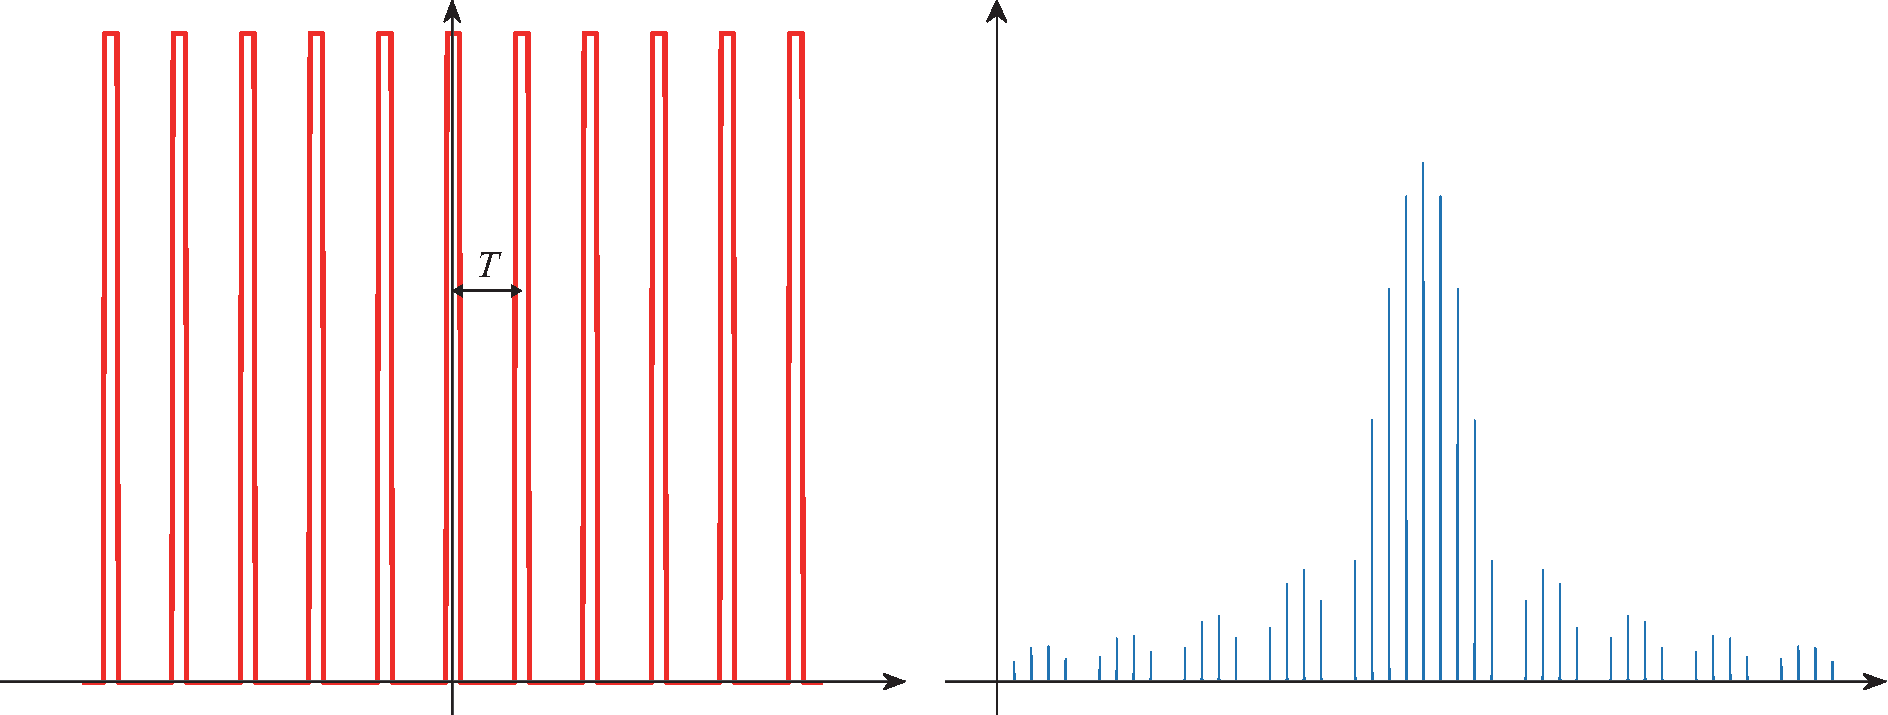
\includegraphics[width=0.5\linewidth]{pic/Fo1.pdf}};
		\node (C) [draw, inner sep = 5pt, below of = B, node distance = 5cm]{\makecell[c]{随着周期的增加,正弦函数的频率\\从稀疏走向密集}};
		\node (C1) [draw, inner sep = 5pt, right of = C, node distance = 9cm]{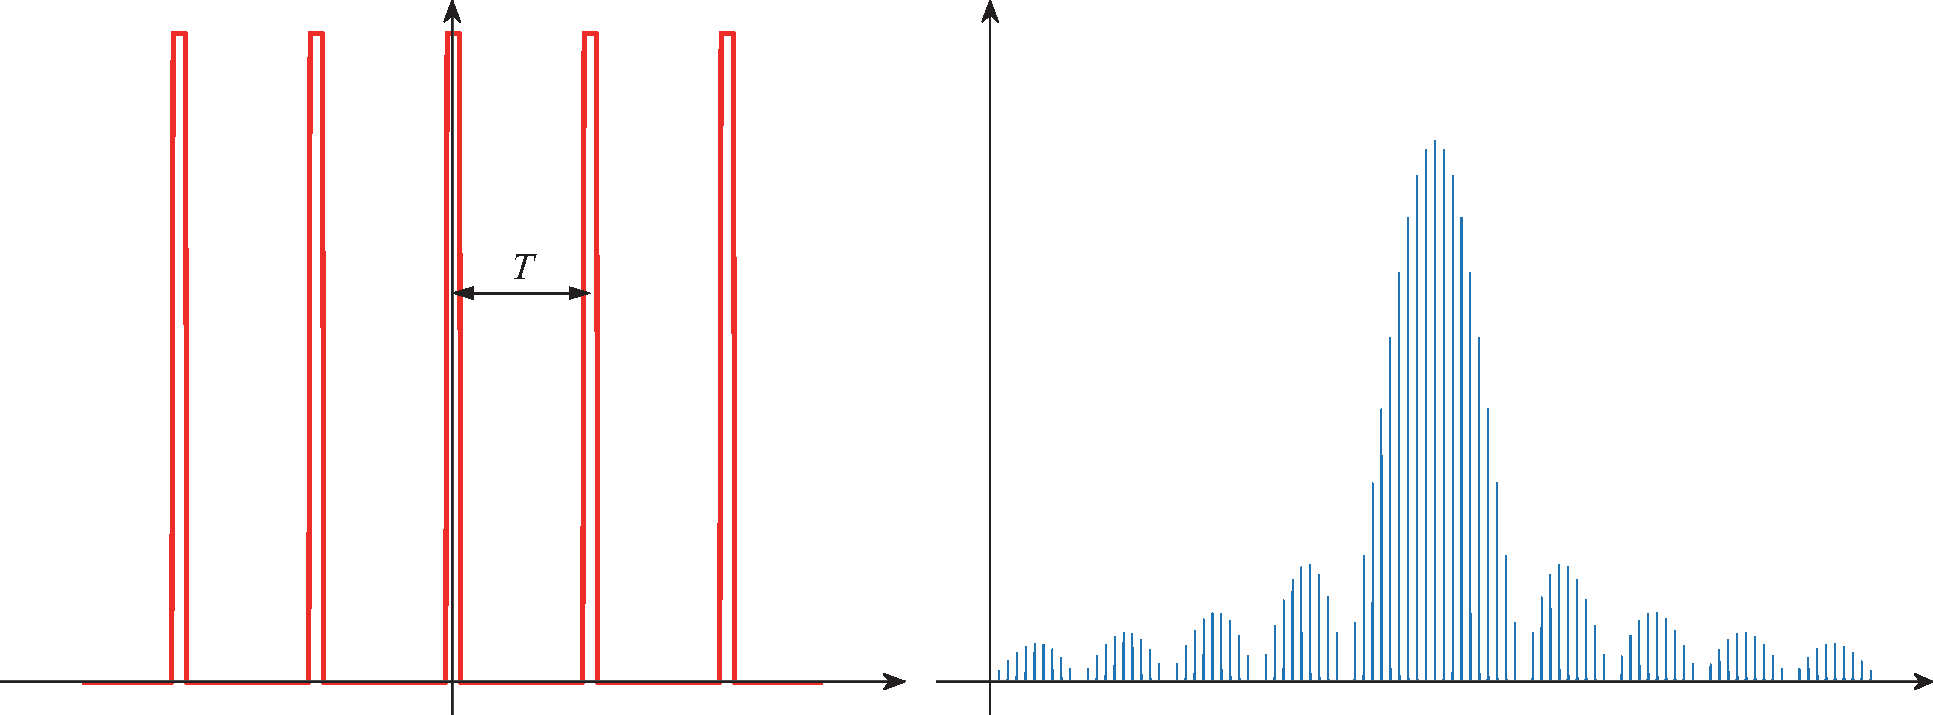
\includegraphics[width=0.5\linewidth]{pic/Fo2.pdf}};
		\node (D) [draw, inner sep = 5pt, below of = C, node distance = 5cm]{\makecell[c]{当周期为无穷大时,正弦函数的频率\\演变为连续的,叠加也由级数变为积分}};
		\node (D1) [draw, inner sep = 5pt, right of = D, node distance = 9cm]{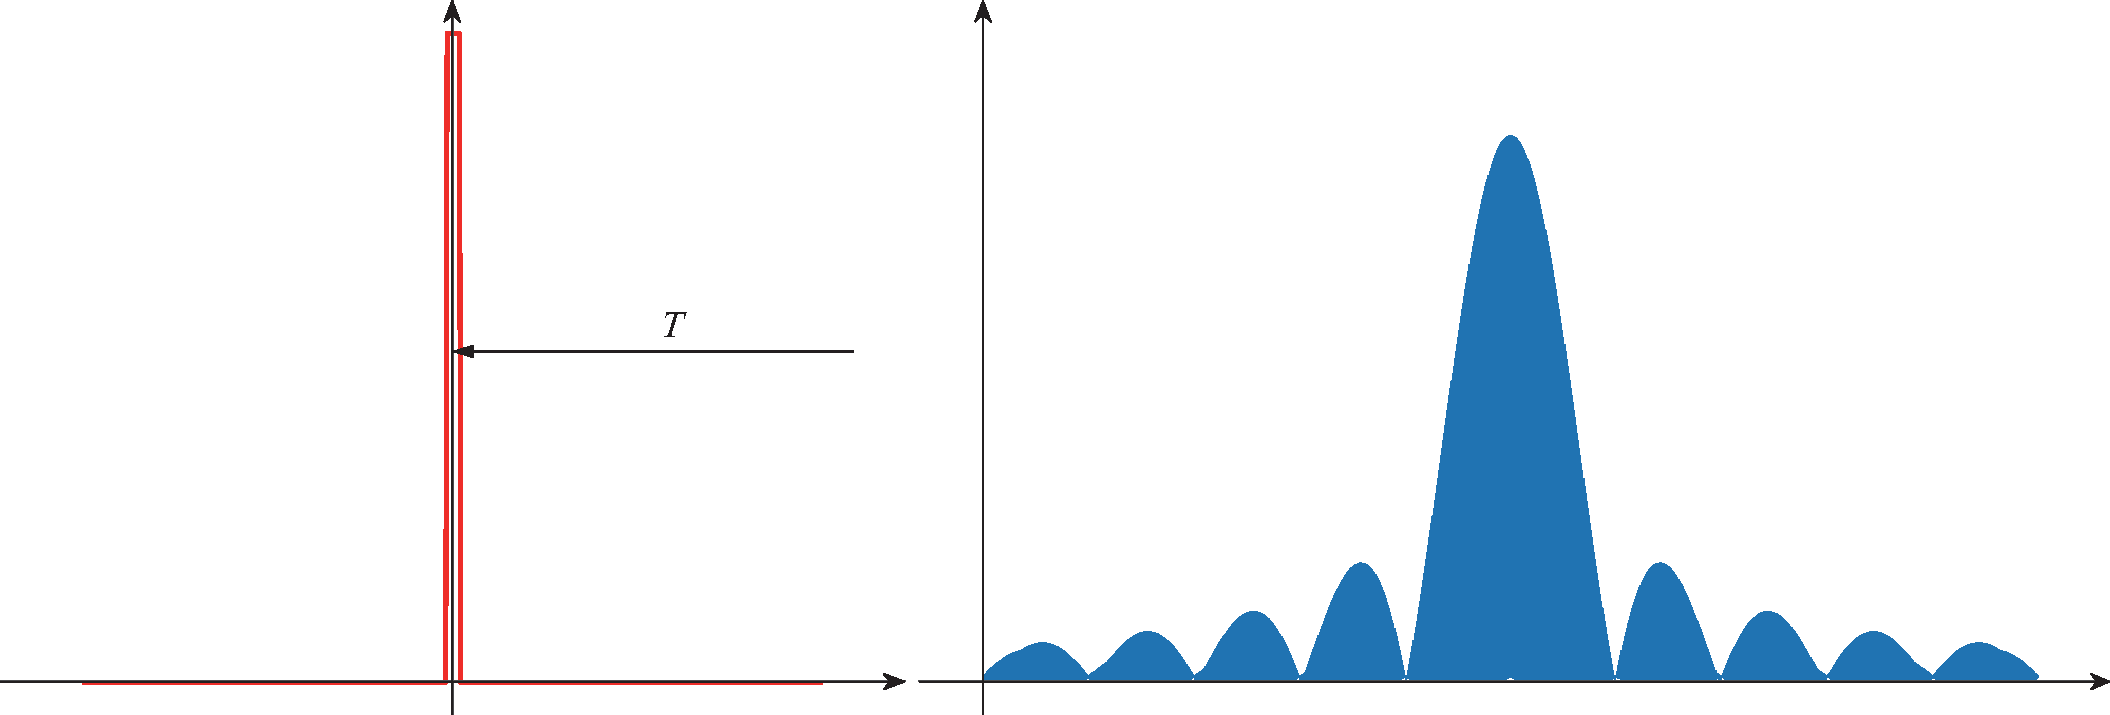
\includegraphics[width=0.5\linewidth]{pic/Fo3.pdf}};
		\node (E) [draw, inner sep = 5pt, below of = D, node distance = 3.5cm]{\makecell[c]{正弦函数又对应圆周运动的投影,\\而$\e^{\i \omega x}$恰好表示频率为$\omega$的单位圆周运动}};
		\node (F) [draw, inner sep = 5pt, right of = E, node distance = 9cm]{\makecell[c]{正弦函数的叠加 $\, \rightarrow \,$ 圆周运动的叠加 $\, \rightarrow \, $ $\e^{\i \omega x}$ 的叠加}};
		\node (G) [draw, inner sep = 5pt, below of = E, node distance = 3.5cm, xshift = 5cm]{$\displaystyle f(x) \sim \mathop{\underbrace{\int_{- \infty}^{+ \infty} \quad \mathop{F(\omega)}_{\makecell[c]{\\[-2em] \scriptsize \mbox{圆周运动的半径}\\[-0.7em] \scriptsize \mbox{和相位信息}\\[-0.7em]}} \quad \mathop{\e^{\i \omega x}}_{\makecell[c]{\scriptsize \mbox{以} {\scriptstyle \omega} \mbox{为频率绕原点}\\[-0.7em] \scriptsize \mbox{做圆周运动的向量}\\[-0.7em]}} \quad \d \omega}}_{\scriptsize \mbox{叠加}}$};
		
		\draw[arrows={-Stealth[scale=0.8]}] (A) -- (B);
		\draw[arrows={-Stealth[scale=0.8]}] (B) -- (C);
		\draw[arrows={-Stealth[scale=0.8]}] (C) -- (D);
		\draw[arrows={-Stealth[scale=0.8]}] (D) -- (E);
		\draw[arrows={-Stealth[scale=0.8]}] (E) --+ (0cm, -1.75cm) --+(5cm, -1.75cm) -- (G);
		\draw[arrows={-Stealth[scale=0.8]}] (F) --+ (0cm, -1.75cm) --+(-4cm, -1.75cm) -- (G);
		\draw (B) -- (B1);
		\draw (C) -- (C1);
		\draw (D) -- (D1);
	\end{tikzpicture}
	\caption{Fourier变换的理解图}
	\label{Fourier变换的理解图}
\end{figure}


\subsection{Fourier变换的基本性质}
\begin{enumerate}[\textbf{性质} 1 ]
	\item \textbf{线性性质} 
	\begin{align}
		\mathcal{F}\big[C_1f_1 + C_2 f_2\big] = C_1 \mathcal{F}\big[f_1\big] + C_2 \mathcal{F}\big[f_2\big] 
	\end{align}
	
	\item \textbf{微分性质}
	\begin{align}
		\mathcal{F}\big[f'(x)\big] &= \i \omega \mathcal{F}\big[f(x)\big]\\[0.5em]
		\mathcal{F}\big[f^{(m)}(x)\big] &= (\i \omega)^{m} \mathcal{F}\big[f(x)\big]
	\end{align}
	
	\item \textbf{象函数微分性质}
	\begin{align}
		\mathcal{F}\big[xf(x)\big] &= \i \dfrac{\d }{\d \omega}\mathcal{F}\big[f(x)\big]\\[0.5em]
		\mathcal{F} \big[x^m f(x)\big] &= \i^m \dfrac{\d^m}{\d \omega^m} \mathcal{F}\big[f(x)\big]
	\end{align}
	
	\item \textbf{卷积性质}
	\begin{itemize}
		\item 卷积定义
		\begin{align}
			f_1(x) * f_2(x) = \int_{- \infty}^{+ \infty} f_1(t)f_2(x - t)\, \d t
		\end{align}
		\item 卷积性质
		\begin{align}
			\mathcal{F}\big[f_1(x) * f_2(x)\big] &= \mathcal{F}\big[f_1(x)\big] \cdot \mathcal{F}\big[f_2(x)\big]\\[0.5em]
			f_1(x) * f_2(x) &= \mathcal{F}^{-1}\big[F_1(\omega)\cdot F_2(\omega)\big]
		\end{align}
	\end{itemize}
\end{enumerate}

\subsection{{$\delta$}函数及其Fourier变换}
\begin{enumerate}[1. ]
	\item $\delta$函数的定义
	\begin{enumerate}[\textbf{特征} 1 ]
		\item \textbf{无穷高且窄}
		\begin{align}
			\delta (x - x_0) = \,
			\begin{cases}
				0, & x \neq x_0\\
				\infty, & x = 0
			\end{cases}
		\end{align}
		
		\item \textbf{具有单位面积}\quad $\displaystyle \int_{- \infty}^{+ \infty} \delta(x - x_0)\, \d x = 1$
	\end{enumerate}
	
	\item $\delta$ 函数的性质
	\begin{enumerate}[\textbf{性质} 1 ]
		\item \textbf{筛选性质} \quad $\displaystyle \int_{- \infty}^{+ \infty} f(x)\delta(x - x_0) \, \d x = f(x_0)$
		\item \textbf{偶函数} \quad $\delta(x) = \delta(-x)$
		\item \textbf{卷积表平移} \quad $\displaystyle \delta(x - a)*f(x) = \int_{- \infty}^{+ \infty} \delta(\xi - a)f(x - \xi) \, \d \xi = f(x - a)$ 
	\end{enumerate}
	
	\item $\delta$函数的Fourier变换
	\begin{align}
		\mathcal{F}\big[\delta(x - x_0)\big] = \int_{-\infty}^{\infty} \delta(x - x_0) \e^{-\i \omega x}\, \d x = 1
	\end{align}
\end{enumerate}
\clearpage

\section{Laplace变换}
\vspace*{1em}
\ttheorem[Laplace变换]
\dy[Laplace变换]{LaplaceBH}
\begin{align}
	F(p) = \mathcal{L}\big[f(t)\big] = \int_{0}^{+ \infty} f(x) \e^{- p t}\, \d x
\end{align}
\vspace*{-2em}

\dy[反演]{FY}
\begin{align}
	f(t) = \mathcal{L}^{-1} \big[F(p)\big] = \dfrac{1}{2 \pi \i} \int_{\beta - \i \infty}^{\beta + \i \infty} F(p) \e^{pt}\, \d p
\end{align}

\subsection{Laplace变换的理解}
\begin{figure}[!htb]
	\centering
	\begin{tikzpicture}
		\node (A) [draw, inner sep = 5pt]{\makecell[c]{我们想求函数$g(t)$的 Fourier变换,然而\\当$t\to \infty, g(t) \to \infty$,不满足绝对可积}};
		\node (AB) [draw, inner sep = 3pt, right of = A, node distance = 7.2cm, yshift = - 2cm]{\makecell[c]{不关心$t<0$时的情况}};
		\node (B) [draw, inner sep = 5pt, below of = A, node distance = 3.5cm]{\makecell[c]{构造新函数}};
		\node (BC) [draw, inner sep = 3pt, right of = B, node distance = 7.5cm, yshift = - 1.75cm]{\makecell[l]{乘以一个衰减函数$\e^{- \beta t}$\\乘以一个单位阶跃函数$u(t)$}};
		\node (C) [draw, inner sep = 7pt, below of = B, node distance = 4cm,]{$g(t) \hspace*{0.5em} \cdot \hspace*{0.5em} \mathop{u(t)}\limits_{\makecell[c]{\\[-2em]\scriptsize \mbox{单位阶跃函数,使}\\[-0.7em] \scriptsize \scriptstyle t < 0\mbox{,函数值为0}\\[-0.7em]}} \hspace*{0.5em} \cdot \hspace*{0.5em} \mathop{\e^{-\beta t}}\limits_{\makecell[c]{\scriptsize \mbox{衰减函数,使}\\[-0.7em] \scriptsize \scriptstyle g(t)\mbox{绝对可积}\\[-0.7em]}}  $};
		\node (CD) [draw, inner sep = 3pt, right of = C, node distance = 7.2cm, yshift = - 2cm]{\makecell[c]{对新函数作Fourier变换}};
		\node (D) [draw, inner sep = 5pt, below of = C, node distance = 3.5cm]{$\displaystyle F(\beta + \i \omega) = \int_{- \infty}^{+ \infty}g(t)u(t)\e^{- \beta t} \e ^{- \i \omega t} \, \d t$};
		\node (DE) [draw, inner sep = 2pt, right of = D, node distance = 6.4cm, yshift = - 2.2cm]{\makecell[l]{$f(t) = g(t) u(t)$ \\ $p = \beta + \i \omega $}};
		\node (E) [draw, inner sep = 5pt, below of = D, node distance = 4cm]{$\displaystyle F(p) = \int_{0}^{+ \infty}f(t) \e ^{- p t} \, \d t$};
		
		\draw[arrows={-Stealth[scale=0.8]}] (A) -- (B);
		\draw[arrows={-Stealth[scale=0.8]}] (B) -- (C);
		\draw[arrows={-Stealth[scale=0.8]}] (C) -- (D);
		\draw[arrows={-Stealth[scale=0.8]}] (D) -- (E);
		\draw[arrows={-Stealth[scale=0.8]}] (AB) -- +(-7.2cm, 0cm);
		\draw[arrows={-Stealth[scale=0.8]}] (BC) -- +(-7.5cm, 0cm);
		\draw[arrows={-Stealth[scale=0.8]}] (CD) -- +(-7.2cm, 0cm);
		\draw[arrows={-Stealth[scale=0.8]}] (DE) -- +(-6.4cm, 0cm);
	\end{tikzpicture}
	\caption{Laplace变换的理解图}
	\label{Laplace变换的理解图}
\end{figure}


\subsection{Laplace变换的性质}

\begin{enumerate}[\textbf{性质} 1 ]
	\item \textbf{线性性质}\\
	若$\alpha,\beta$是任意常实数,且$\mathcal{L}\big[f_1(t)\big] = F_1(s), \mathcal{L}\big[f_2(t)\big] = F_2(s)$,则有
	\begin{equation}
		\mathcal{L}\big[\alpha f_1(t)\pm \beta f_2(t)\big] = \alpha F_1(s) \pm \beta F_2(s)
	\end{equation}
	
	\item \textbf{微分性质}\\
	若$\mathcal{L}\big[f(t)\big] = F(s)$,则有
	\begin{equation}
		\mathcal{L}\big[f^{(n)}(t)\big] = s^nF(s) -s^{n-1}f(0)-s^{n-2}f'(0)- \cdots - f^{(n-1)}(0)
	\end{equation}
	
	\item \textbf{积分性质}\\
	若$\mathcal{L}\big[f(t)\big] = F(s)$,则有
	\begin{equation}
		\mathcal{L}\left[\underbrace{\int\cdots\int}_{n} f(t) \,\d t^n\right]=\frac{1}{s^n}F(s)+\frac{1}{s^n}f^{-1}(0) +\frac{1}{s^{n-1}}f^{(-2)}(0)+\cdots +\frac{1}{s}f^{(-n)}(0)
	\end{equation}
	其中,$f^{(-1)}(0),f^{(-2)}(0),f^{(-n)}(0)$分别为$f(t)$的各重积分在$t=0$处的值。\\
	
	\item \textbf{卷积定理}\\
	若$\mathcal{L}\big[f_1(t)\big] = F_1(s), \mathcal{L}\big[f_2(t)\big] = F_2(s)$,则
	\begin{equation}
		\mathcal{L}\big[f_1(t) * f_2(t)\big] = F_1(s) \cdot F_2(s)
	\end{equation}
\end{enumerate}
\warn[
Laplace变换的重要条件:\vspace*{-0.5em}
{
	\begin{enumerate}
		\item $t<0$时,$f(t)=0$;$t > 0$时,$f(t)$是分段光滑的。\vspace*{-0.5em}
		\item $f(t)$有\textcolor{red}{有限的增长指数}。即存在正数$M$及$c \ge 0$,使得对于任何$t$值,$|f(t)| \le M\e^{ct}$,则Laplace变换在$\text{Re} (p)= \beta >c$时存在。
	\end{enumerate}
}
]

\subsection{Laplace反演的计算}
\noindent \textbf{1. 留数定理}
\begin{enumerate}[\hspace*{2em}(1) ]
	\item 极点的判断方法:\textbf{$\dfrac{1}{f(p)}$的$m$重零点就是$f(p)$的$m$级极点}.
	\item $n$级极点的留数:设$p_0$是函数$f(p)$的$n$级极点,则
	\begin{equation}
		\text{Res} [f(p), p_0] = \dfrac{1}{(n-1)!} \lim\limits_{p \to p_0} \dfrac{\d^{n-1}\big[(p - p_0)^n f(p)\big]}{\d p^{n-1}}
	\end{equation}
\end{enumerate}


\noindent \textbf{2. 反演公式转换为求极点留数}

设$p_1,p_2,\cdots,p_n$是函数$F(p)$的所有奇点,适当选取$\Re (p) = \beta$使这些奇点落在复平面上直线$\Re(p) = \beta$的左侧,且$\bm{p \to \infty,  F(p) \to 0}$,则
\begin{align}
	f(t) = \sum_{k = 0}^n \text{Res}\big[F(p)\e^{pt}, p_k\big]
\end{align}

\subsection{Laplace变换的应用——求解常微分方程(组)}
\texample[Laplace变换求解常微分方程(组)]\vspace*{2em}
\noindent \vspace*{1.5em} \noindent  \hspace*{0.2em}  \tcbox[colframe =black, colback =black!10!white,boxrule=0.5mm,size=small,on line]{\color{black}{{ 解题步骤}}\hspace*{0.25em}}\hspace{1.5em}
\vspace*{-1em}
\begin{enumerate}
	\item 对方程两边同时做拉普拉斯变换。
	\item 利用拉普拉斯变换的线性性质、微分性质代替各阶的的导数,解出$Y(s)$。
	\item 做$Y(s)$的拉普拉斯逆变换,得到$y(t)$。
\end{enumerate}
\warn[
\textbf{Fourier变换和Laplace变换的对比}\vspace*{-0.5em}
{
	\begin{enumerate}
		\item 都属于积分变换,实函数变换为复函数,但积分范围不同。\vspace*{-0.5em}
		\item 存在条件\vspace*{-0.5em}
		\begin{itemize}
			\item Fourier \quad 分段光滑,绝对可积
			\item Laplace \quad 分段光滑,$f(t)$增长小于指数级
		\end{itemize}
		\item 积分变量不同\vspace*{-0.5em}
		\begin{itemize}
			\item Fourier \quad $\omega \in (- \infty , + \infty)$
			\item Laplace \quad $p$的实部满足一定条件(可自行调节)
		\end{itemize}
	\end{enumerate}
}
]

\section{积分变换法}
\subsection{积分变换法简述}
\noindent \textbf{1. 积分变换的性质}
\begin{enumerate}[\hspace*{1em}\textbf{性质} 1 ]
	\item \textbf{积分变换的微分性质}
	\begin{align}
		\mathcal{F}\big[f'(x)\big] &=  \i \omega \mathcal{F}\big[f(x)\big] \\[0.5em]
		\mathcal{F}\big[f''(x)\big] &=  -\omega^2 \mathcal{F}\big[f(x)\big] \\[1em]
		\mathcal{L}\big[f'(t)\big] & = p \mathcal{L}\big[f(t)\big] - f(0)\\[0.5em]
		\mathcal{L}\big[f''(t)\big] & = p^2\mathcal{L}\big[f(t)\big] - pf(0) - f'(0)
	\end{align}
	
	\item \textbf{积分变换的卷积性质}
	\begin{align}
		f_1(x) * f_2(x) &= \int_{-\infty}^{+\infty} f_1(\xi)f_2(x - \xi) \, \d \xi  = \mathcal{F}^{-1}\big[F_1(\omega)\cdot F_2(\omega)\big]\\[1em]
		f_1(t) * f_2(t) &= \int_{0}^{t} f_1(\tau)f_2(t - \tau) \, \d \tau = \mathcal{L}^{-1}\big[F_1(p)\cdot F_2(p)\big]
	\end{align}
\end{enumerate}

\noindent \textbf{2. 积分变换法的基本步骤}
\begin{enumerate}[\hspace*{1em}\textbf{步骤} 1 ]
	\item \textbf{变换} \quad 选适当的积分变换,对方程的两边做变换将偏微分方程变为含参量的常微分方程;对变换中未利用到的定解条件也做变换。关于积分变量的选取,与两个变换方法的积分域有关:
	\begin{itemize}
		\item Fourier变换 \quad 积分域为$(-\infty, + \infty) \quad \Rightarrow \quad$无界空间变量
		\item Laplace变换 \quad 积分域为$(0, +\infty) \quad \Rightarrow \quad$时间变量
		\item 如果同时存在无界空间变量和时间变量,这时可以联用两种变换,即\dy[联合变换]{LHBH}
	\end{itemize}
	\item \textbf{求解} \quad 解常微分方程,得到像函数的解
	\begin{itemize}
		\item 一阶齐次方程 \quad 分离变量法
		\item 二阶齐次方程\quad 特征根法
		\item 非齐次方程\quad 常数变易法
	\end{itemize}
	\item \textbf{反演} \quad 对像函数反演,得到原定解问题的解,通常有以下两个解法
	\begin{itemize}
		\item 查表$+$卷积性质
		\item 留数定理
	\end{itemize}
\end{enumerate}
\vspace*{-1em}

\warn[
\begin{itemize}
	\item 在用积分变换求解定解问题时,假定所求的解及定解条件 中的已知函数的变换都是存在的;\vspace*{-0.5em}
	\item 一个未知函数在未求出前是很难判断变换是否存在的,因此,在未做验证前,得到的只是形式解。
\end{itemize}
]

\subsection{积分变换法举例}
\begin{equation*}
	\mbox{积分变换法} \, 
	\begin{cases}
		\, \mbox{热传导方程} \,
		\begin{cases}
			\, \mbox{无界杆的热传导问题}\\
			\, \mbox{半无界杆的热传导问题}\\
		\end{cases}
		\\
		\, \mbox{波动方程} \,
		\begin{cases}
			\, \mbox{无界弦的自由振动}\\
			\, \mbox{无界弦的受迫振动}\\
			\, \mbox{有界杆的受迫振动}
		\end{cases}
	\end{cases}
\end{equation*}
\vspace*{1em}

\example[无界杆上的热传导问题]
设有一个根无限长的杆,杆上具有强度为$F(x,t)$的热源,杆的初始温度为$\varphi(x)$,试求$t>0$时杆上温度的分布规律。

\solve 方法一:Fourier变换
\begin{enumerate}[\textbf{第} 1 \textbf{步} ]
	\item \textbf{列出定解问题}
	\begin{equation}
		\begin{cases}
			\, \dfrac{\partial u}{\partial t} = a^2 \dfrac{\partial^2 u}{\partial x^2} + f(x,t), & -\infty < x< +\infty,t>0\\[0.5em]
			\, u|_{t = 0} = \varphi(x), & -\infty < x < + \infty
		\end{cases}
	\end{equation}
	其中,$\displaystyle a^2 \dfrac{\lambda}{\rho c}$表示热扩散系数,$f(x,t) = \dfrac{F(x,t)}{\rho c}$.可以分析得到:
	\begin{itemize}
		\item 具有无界空间变量$x$,可进行Fourier变换;
		\item 具有时间变量$t$,可进行Laplace变换;
		\item 可以单独采用一种变换,也可以两种联用;
	\end{itemize}
	
	\item \textbf{变换}
	\begin{itemize}
		\item 取$x$为变换变量,对方程和定解条件进行Fourier变换
		\begin{equation}
			\begin{cases}
				\, \dfrac{\displaystyle \partial \int_{-\infty}^{+\infty} u(x,t)\e^{- \i \omega x} \, \d x}{\partial t} = \displaystyle a^2 \int_{- \infty}^{+ \infty} \dfrac{\partial^2 u(x,t)}{\partial x^2} \e^{- \i \omega x}\, \d x + \int_{- \infty}^{+\infty}\e^{- \i \omega x} \, \d x\\[1em]
				\, \displaystyle \int_{-\infty}^{+\infty} u(x,0) \e^{- \i \omega x}\, \d x = \int_{- \infty}^{+ \infty}\varphi(x)\e^{-\i \omega x} \, \d x
			\end{cases}
		\end{equation}
		
		\item 记$U = \mathcal{F}[u], G = \mathcal{F}[f], \varPhi = \mathcal{F}[\varphi]$,则
		\begin{equation}
			\begin{cases}
				\, \dfrac{\d U(\omega, t)}{\d t} = - a^2 \omega^2U(\omega, t) + G(\omega, t)\\
				\, U(\omega, t)|_{t = 0} = \varPhi(\omega)
			\end{cases}
		\label{无界杆传热}
		\end{equation}
	\end{itemize}
	
	\item \textbf{求解}\\
	方程\eqref{无界杆传热}是以$\omega$为参变量的一阶线性非齐次常微分方程,利用常数变易法解得
	\begin{equation}
		U(\omega, t) = \varPhi(\omega)\exp\left(-a^2 \omega^2 t\right) + \int_0^t G(\omega ,\tau) \exp \big[-a^2 \omega^2(t - \tau)\big]\, \d \tau
	\end{equation}
	
	\item \textbf{反演}
	\begin{itemize}
		\item 查表可得
		\[
		\begin{cases}
			\, \mathcal{F}^{-1}\left[\exp\left(-a^2 \omega^2 t\right)\right] = \dfrac{1}{2a\sqrt{\pi t}}\exp \left(-\dfrac{x^2}{4a^2t}\right)\\[1em]
			\, \mathcal{F}^{-1}\bigg\lbrace\exp\left[-a^2 \omega^2 (t-\tau)\right]\bigg\rbrace = \dfrac{1}{2a\sqrt{\pi (t-\tau)}}\exp \left(-\dfrac{x^2}{4a^2(t - \tau)}\right)
		\end{cases}
		\]
		
		\item 卷积性质
		\begin{align}
			u(x,t) &= \varphi(x) * \Bigg[\dfrac{1}{2 a \sqrt{\pi t}}\exp\left(-\dfrac{x^2}{4a^2t}\right)\Bigg]\notag \\[1em]
			&\quad +\int_{0}^{t} \Bigg\lbrace f(x, \tau) * \dfrac{1}{2a\sqrt{\pi (t - \tau)}}\exp \left[-\dfrac{x^2}{4a^2(t - \tau)}\right] \Bigg \rbrace \, \d \tau \notag \\[1em]
			& = \dfrac{1}{2a\sqrt{\pi t}}\int_{-\infty}^{+\infty}\varphi(\xi)\exp\left[-\dfrac{(x - \xi)^2}{4a^2t}\right]\, \d \xi \notag\\[1em]
			&\quad + \dfrac{1}{2a \sqrt{\pi}} \int_0^t\int_{-\infty}^{+\infty}\dfrac{f(\xi, \tau)}{\sqrt{t - \tau}} \exp \left[-\dfrac{(x - \xi)^2}{4a^2(t - \tau)}\right]\, \d \xi \d \tau
		\end{align}
	\end{itemize}
\end{enumerate}

	\solveother 方法二:联合变换求解
\begin{enumerate}[\textbf{第} 1 \textbf{步} ]
	\item \textbf{列出定解问题}
	\begin{equation}
		\begin{cases}
			\, \dfrac{\partial u}{\partial t} = a^2 \dfrac{\partial^2 u}{\partial x^2} + f(x,t), & -\infty < x< +\infty,t>0\\[0.5em]
			\, u|_{t = 0} = \varphi(x), & -\infty < x < + \infty
		\end{cases}
	\end{equation}
	\item \textbf{变换}
		\begin{itemize}
			\item 取$x$为变换变量,对方程和定解条件进行Fourier变换,记$U = \mathcal{F}[u], G = \mathcal{F}[f], \varPhi = \mathcal{F}[\varphi]$,则
			\begin{equation}
				\begin{cases}
					\, \dfrac{\d U(\omega, t)}{\d t} = - a^2 \omega^2U(\omega, t) + G(\omega, t)\\
					\, U(\omega, t)|_{t = 0} = \varPhi(\omega)
				\end{cases}
			\end{equation}
			\item 再对变量$t$作Laplace变换:
			\begin{equation}
				\int_{0}^{\infty} \dfrac{\d U(\omega, t)}{\d t} \e^{- p t} \, \d t = -a^2\omega^2\int_{0}^{\infty} U(\omega, t)\e^{-p t} \, \d t + \int_{0}^{\infty}G(\omega, t)\e^{-pt}\, \d t
			\end{equation}
		\end{itemize}	
	引入$\sim$符号表示像函数,得到代数方程
	\begin{equation}
		p \widetilde{U}(\omega , p) - \varPhi(\omega) = -a^2 \omega^2 \widetilde{U}(\omega, p) + \widetilde{G}(\omega, p)
		\label{无界杆传热2}
	\end{equation}
	
	\item \textbf{求解}\\
	方程\eqref{无界杆传热2}是线性方程,直接解得
	\begin{equation}
		\widetilde{U}(\omega, p) = \dfrac{1}{p + a^2 \omega^2}\varPhi(\omega) + \dfrac{1}{p + a^2 \omega^2} \widetilde{G}(\omega, p)
	\end{equation}
	
	\item \textbf{反演}\\
	(1) 先对变量$p$进行反演
	\begin{itemize}
		\item 查表可得
		\[
		\mathcal{L}^{-1}\left[\dfrac{1}{p + a^2 \omega^2}\right] = \exp\left(-a^2 \omega^2 t\right)
		\]
		
		\item 卷积性质
		\begin{align}
			U(\omega, p) &= \mathcal{L}^{-1}\left[\dfrac{1}{p + a^2 \omega^2}\varPhi(\omega) + \dfrac{1}{p + a^2 \omega^2} \widetilde{G}(\omega, p)\right] \notag\\
			& = \varPhi(\omega) \exp\left(-a^2 \omega^2 t\right) + G(\omega, t)*\exp\left(-a^2 \omega^2 t\right) \notag\\
			& = \varPhi(\omega) \exp\left(-a^2 \omega^2 t\right) + \int_0^t G(\omega, t)*\exp\left[-a^2 \omega^2 (t - \tau)\right]\, \d \tau
		\end{align}
	\end{itemize}
	(2) 再对变量$\omega$进行反演,此步骤与方法一完全相同,略。
\end{enumerate}
\vspace*{4em}

\example[半无界杆上的热传导问题]
设有一根半无限长的杆,端点温度变化为已知,杆的初始温度为$0\degree \text{C}$,求杆上的温度分布规律。

\solve 利用Laplace变换求解
\begin{enumerate}[\textbf{第} 1 \textbf{步} ]
	\item \textbf{列出定解问题}
	\begin{equation}
		\begin{cases}
			\, \dfrac{\partial u}{\partial t} = a^2 \dfrac{\partial^2 u}{\partial x^2}, & x>0,t>0\\
			\, u|_{x = 0} = f(t), & t > 0\\
			\, u|_{t = 0} = 0, & x > 0
		\end{cases}
	\end{equation}
	\clearpage
	可以分析得到:
	\begin{itemize}
		\item 没有无界空间变量$x$,不可以进行Fourier变换;
		\item 具有时间变量$t$,可进行Laplace变换。
	\end{itemize}
	
	\item \textbf{变换}
	\begin{itemize}
		\item 取$t$为变换变量,对方程和定解条件进行Laplace变换
		\begin{equation}
			\begin{cases}
				\, \dfrac{\displaystyle \partial \int_{0}^{+\infty} u(x,t)\e^{- p t} \, \d t}{\partial t} = \displaystyle a^2 \int_{0}^{+ \infty} \dfrac{\partial^2 u(x,t)}{\partial x^2} \e^{- p t}\, \d t \\[1em]
				\, \displaystyle \int_{0}^{+\infty} u(0,t) \e^{- p t}\, \d t = \int_{0}^{+ \infty}f(t)\e^{-pt} \, \d t
			\end{cases}
		\end{equation}
		
		\item 记$U = \mathcal{L}[u],F = \mathcal{L}[f]$,则
		\begin{equation}
			\begin{cases}
				\, \dfrac{\d^2 U(x, p)}{\d x^2} - \dfrac{p}{a^2} U(\omega, t) = 0 \\
				\, U(x, p)|_{x = 0} = F(p)
			\end{cases}
			\label{半无界杆传热}
		\end{equation}
	\end{itemize}
	
	\item \textbf{求解}\\
	方程\eqref{半无界杆传热}是以$p$为参变量的一阶线性齐次常微分方程,利用特征根法得其通解为
	\begin{equation}
		U(x, p) = C_1 \exp \left(\dfrac{\sqrt{p}}{a}x\right) + C_2\exp \left(-\dfrac{\sqrt{p}}{a}x\right) 
	\end{equation}
	由于$x \to \infty, U \to C$(常数),所以为了保证$U(x, p)$的有界性,无穷发散量$\exp \left(\dfrac{\sqrt{p}}{a}x\right)$的系数$C_1 = 0.$
	
	再根据边界条件得到方程的特解
	\begin{equation}
		U(x, p) = F(p) \exp\left(-\dfrac{p}{a^2}x\right)
	\end{equation}
	
	\item \textbf{反演}
	\begin{itemize}
		\item 查表可得
		\[
		\mathcal{L}\Bigg[\text{erfc}\left(\dfrac{x}{2a\sqrt{t}}\right)\Bigg] = \dfrac{1}{p}\exp \left(-\dfrac{\sqrt{p}}{a}\right)
		\]
		
		\item 微分性质
		\[
		\mathcal{L} \Bigg[\dfrac{\d }{\d t}\text{erfc}\left(\dfrac{x}{2a\sqrt{t}}\right)\Bigg] = p \mathcal{L}\Bigg[\text{erfc}\left(\dfrac{x}{2a\sqrt{t}}\right)\Bigg] - \text{erfc}(\infty) = p \cdot \dfrac{1}{p}\exp \left(-\dfrac{\sqrt{p}}{a}\right) - 0 = \exp \left(-\dfrac{\sqrt{p}}{a}\right) 
		\]
		所以
		\begin{equation}
			\mathcal{L}^{-1}  \Bigg[\exp \left(-\dfrac{\sqrt{p}}{a}\right)  \Bigg] = \dfrac{\d }{\d t}\text{erfc}\left(\dfrac{x}{2a\sqrt{t}}\right) = \dfrac{x}{2a \sqrt{\pi} t^{3/2}}\exp \left(-\dfrac{x^2}{4a^2t}\right)
		\end{equation}
		
		\item 卷积性质
		\begin{equation}
			u(x, t) = \mathcal{L}^{-1}\big[U(x, p)\big] = \dfrac{x}{2a \sqrt{\pi}}\int_0^t \dfrac{f(\tau)}{(t - \tau)^{3/2}} \exp \left[- \dfrac{x^2}{4a^2(t - \tau)}\right]\, \d \tau
		\end{equation}
	\end{itemize}
\end{enumerate}
\clearpage

\example[无界弦的自由振动]
试分析无界弦的自由振动。

\solve 利用Fourier变换求解
\begin{enumerate}[\textbf{第} 1 \textbf{步} ]
	\item \textbf{列出定解问题}
	\begin{equation}
		\begin{cases}
			\, \dfrac{\partial^2 u}{\partial t^2} = a^2 \dfrac{\partial^2 u}{\partial x^2} , & -\infty < x< +\infty,t>0\\[0.5em]
			\, u|_{t = 0} = \varphi(x), & -\infty < x < + \infty\\[0.5em]
			\,\left. \dfrac{\partial u}{\partial t}\right|_{t = 0} = \psi(x), & -\infty < x < +\infty
		\end{cases}
	\end{equation}
	可以分析得到:
	\begin{itemize}
		\item 具有无界空间变量$x$,可进行Fourier变换;
		\item 具有时间变量$t$,可进行Laplace变换;
		\item 可以单独采用一种变换,也可以两种联用;
	\end{itemize}
	
	\item \textbf{变换}
	\begin{itemize}
		\item 取$x$为变换变量,对方程和定解条件进行Fourier变换
		\begin{equation}
			\begin{cases}
				\, \displaystyle \dfrac{\partial^2}{\partial t^2} \int_{-\infty}^{+\infty} u(x,t)\e^{- \i \omega t} = a^2 \int_{- \infty}^{+\infty} \dfrac{\partial^2 u(x,t)}{\partial x^2} \e^{- \i \omega x}\,\d x \\[1em]
				\, \displaystyle \left[\int_{- \infty}^{+\infty}u(x,t)\e^{-\i \omega x}\, \d x\right]_{t = 0} = \int_{-\infty}^{+ \infty} \varphi(x)\, \d x \\[1em]
				\, \displaystyle \left[\int_{- \infty}^{+\infty} \dfrac{\partial u(x,t)}{\partial t}\e^{- \i \omega x}\, \d x\right]_{t = 0} = \int_{- \infty}^{+\infty} \psi(x)\e^{- \i \omega x} \, \d x
			\end{cases}
		\end{equation}
		
		\item 记$U = \mathcal{F}[u], \varPhi = \mathcal{F}[\varphi], \varPsi = \mathcal{F}[\psi]$,则
		\begin{equation}
			\begin{cases}
				\, \displaystyle \dfrac{\d^2 U(\omega, t)}{\d t^2} = -a^2 \omega^2 U(\omega, t)\\[0.5em]
				\, \displaystyle U(\omega, t)|_{t = 0} = \varPhi(\omega)\\[0.5em]
				\, \displaystyle \left. \dfrac{\d U(\omega, t)}{\d t} \right|_{t = 0} = \varPsi(\omega)
			\end{cases}
			\label{无界弦自由振动}
		\end{equation}
	\end{itemize}
	
	\item \textbf{求解}\\
	方程\eqref{无界弦自由振动}是以$\omega$为参变量的二阶线性齐次常微分方程,利用特征根法解得
	\begin{itemize}
		\item 通解
		\begin{equation}
			U(\omega, t) = A\cos a\omega t + B\sin a \omega t
		\end{equation}
		\item 特解
		\begin{equation}
			U(\omega, t) = \varPhi(\omega)\cos a\omega t + \varPsi(\omega) \dfrac{\sin a\omega t}{a \omega}
		\end{equation}
	\end{itemize}
	
	\item \textbf{反演}
	\begin{itemize}
		\item 利用欧拉公式变形
		\begin{align*}
			U(\omega, t) & = \varPhi(\omega)\cos a\omega t + \Psi(\omega)\dfrac{\sin a\omega t}{a \omega} \\
			& = \dfrac{1}{2}\big[\varPhi(\omega) \e^{\i a \omega t} + \varPhi(\omega)\e^{- \i a \omega t}\big] + \dfrac{1}{2a} \Bigg[\dfrac{1}{\i \omega}\varPsi(\omega) \e^{\i a \omega t} - \dfrac{1}{\i \omega} \varPsi(\omega) \e^{- \i a\omega t}\Bigg]
		\end{align*}
		\item 位移性质
		\begin{equation}
			f(x + x_0) = \mathcal{F}^{-1} \big[\e^{\i \omega x_0}F(\omega)\big]
		\end{equation}
		
		\item 积分性质
		\begin{equation}
			\int_{-\infty}^x f(\xi) \, \d \xi = \mathcal{F}^{-1} \Bigg[\dfrac{1}{\i \omega}F(\omega)\Bigg]
		\end{equation}
		
		\item 将位移性质作用于积分性质
		\begin{equation}
			\int_{-\infty}^{x + x_0} f(\xi)\, \d \xi = \mathcal{F}^{-1} \Bigg[\dfrac{1}{\i \omega} F(\omega) \e^{\i \omega x_0}\Bigg]
		\end{equation}
		
		所以
		\begin{align}
			u(x, t) &= \dfrac{1}{2} \big[\varphi(x + at) + \varphi(x - at)\big] + \dfrac{1}{2a}\Big[\int_{- \infty}^{x +at}\psi(\xi)\, \d \xi - \int_{-\infty}^{x - at} \psi(\xi) \, \d \xi\Big]\notag \\[1em]
			& = \dfrac{1}{2}\big[\varphi(x + at) + \varphi(x - at)\big] + \dfrac{1}{2a} \int_{x-at}^{x+at}\psi(\xi) \, \d \xi
		\end{align}
	\end{itemize}
\end{enumerate}

\example[无界弦的受迫振动]
试分析无界弦的受迫振动。

\solve 利用Fourier变换求解
\begin{enumerate}[\textbf{第} 1 \textbf{步} ]
	\item \textbf{列出定解问题}
	\begin{equation}
		\begin{cases}
			\, \dfrac{\partial^2 u}{\partial t^2} = a^2 \dfrac{\partial^2 u}{\partial x^2} + f(x,t), & -\infty < x< +\infty,t>0\\[0.5em]
			\, u|_{t = 0} = 0, & -\infty < x < + \infty\\[0.5em]
			\,\left. \dfrac{\partial u}{\partial t}\right|_{t = 0} = 0, & t-\infty < x < +\infty
		\end{cases}
	\end{equation}
	可以分析得到:
	\begin{itemize}
		\item 具有无界空间变量$x$,可进行Fourier变换;
		\item 具有时间变量$t$,可进行Laplace变换;
		\item 可以单独采用一种变换,也可以两种联用;
	\end{itemize}
	
	\item \textbf{变换}
	\begin{itemize}
		\item 取$x$为变换变量,对方程和定解条件进行Fourier变换
		\begin{equation}
			\begin{cases}
				\, \displaystyle \dfrac{\partial^2}{\partial t^2} \int_{-\infty}^{+\infty} u(x,t)\e^{- \i \omega t} = a^2 \int_{- \infty}^{+\infty} \dfrac{\partial^2 u(x,t)}{\partial x^2} \e^{- \i \omega x}\,\d x + \int_{- \infty}^{+\infty} f(x,t) \e^{- \i \omega x}\,\d x\\[1em]
				\, \displaystyle \left[\int_{- \infty}^{+\infty}u(x,t)\e^{-\i \omega x}\, \d x\right]_{t = 0} = 0\\[1em]
				\, \displaystyle \left[\int_{- \infty}^{+\infty} \dfrac{\partial u(x,t)}{\partial t}\e^{- \i \omega x}\, \d x\right]_{t = 0} = 0\,
			\end{cases}
		\end{equation}
		
		\item 记$U = \mathcal{F}[u], F= \mathcal{F}[f]$,则
		\begin{equation}
			\begin{cases}
				\, \displaystyle \dfrac{\d^2 U(\omega, t)}{\d t^2} = -a^2 \omega^2 U(\omega, t) + F(\omega, t)\\[0.5em]
				\, \displaystyle U(\omega, t)|_{t = 0} = 0\\[0.5em]
				\, \displaystyle \left. \dfrac{\d U(\omega, t)}{\d t} \right|_{t = 0} = 0
			\end{cases}
			\label{无界弦受迫振动}
		\end{equation}
	\end{itemize}
	
	\item \textbf{求解}\\
	方程\eqref{无界弦受迫振动}是以$\omega$为参变量的二阶线性非齐次常微分方程,利用常数变易法解得
		\begin{equation}
			U(\omega, t) = \dfrac{1}{a} \int_0^t F(\omega, t) \dfrac{\sin a\omega(t-\tau)}{\omega}\, \d \tau
		\end{equation}
	
	\item \textbf{反演}
	\begin{itemize}
		\item 查表,得
		\[
		\mathcal{F} \left[ f(x) =\, 
		\begin{cases}
			\, h, &- \tau < t < \tau\\
			\, 0, &\text{others}
		\end{cases}
		\right]
		 = 2h \dfrac{\sin \omega \tau}{\omega}
		\]
		经过变量替换,得到
		\[
		\dfrac{\sin a\omega(t - \tau)}{\omega} = \mathcal{F} \left[
		g(x) = \,
		\begin{cases}
			\, \dfrac{1}{2}, & -a(t - \tau) < x < a(t - \tau)\\
			\, 0, & \text{others}
		\end{cases}
		\right]
		\]
		\item 由卷积性质
		\begin{align}
			u(x, t) &= \dfrac{1}{2a} \int_0^t f(x,\tau) *g(x)\,\d \tau = \dfrac{1}{a} \int_0^t \int_{-\infty}^{+\infty} f(\xi, \tau) g(x - \xi) \, \d \xi \d \tau\\[0.5em]
			& = \dfrac{1}{2a} \int_{x-a(t - \tau)}^{x+a(t - \tau)}f(\xi, \tau) \, \d \xi
		\end{align}
	\end{itemize}
\end{enumerate}

\example[有界杆的受迫振动]
设有一根长为$l$的均匀杆,其一端固定,另一端由静止状态开始受力$F = A \sin \omega t$的作用,力$F$的方向与杆的轴线一致,求杆在零初值条件下作纵振动的规律。

\solve 利用Laplace变换求解
\begin{enumerate}[\textbf{第} 1 \textbf{步} ]
	\item \textbf{列出定解问题}
	\begin{equation}
		\begin{cases}
			\, \dfrac{\partial^2 u}{\partial t^2} = a^2 \dfrac{\partial^2 u}{\partial x^2} , & 0 < x< l,t>0\\[1em]
			\, u|_{t = 0} = 0, 	\,\left. \dfrac{\partial u}{\partial t}\right|_{t = 0} = 0, & 0 \le x \le l\\[1em]
			\, u|_{x = 0} = 0, 	\,\left. \dfrac{\partial u}{\partial t}\right|_{x = l} = \dfrac{A}{E}\sin \omega t, & t>0
		\end{cases}
	\end{equation}
	可以分析得到:
	\begin{itemize}
		\item 不具有无界空间变量$x$,不可进行Fourier变换;
		\item 具有时间变量$t$,可进行Laplace变换;
	\end{itemize}
	
	\item \textbf{变换}
	\begin{itemize}
		\item 取$t$为变换变量,对方程和定解条件进行Laplace变换
		\begin{equation}
			\begin{cases}
				\, \displaystyle \int_0^{+\infty} \dfrac{\partial^2 u(x,t)}{\partial t^2}\e^{-p t}\, \d t = a^2 \dfrac{\partial^2 }{\partial x^2} \int_0^{+\infty} u(x,t)\e^{- p t}\, \d t,\\[1em]
				\, \displaystyle \int_0^{+\infty} u(0,t) \e^{-pt}\, \d t = 0,\\[1em]
				\, \displaystyle \dfrac{\partial }{\partial x}\int_0^{+\infty} u(l,t)\e^{-pt}\, \d t = \dfrac{A}{E} \sin \omega t 
			\end{cases}
		\end{equation}
		
		\item 记$U = \mathcal{L}[u]$ 则
		\begin{equation}
			\begin{cases}
				\, \displaystyle p^2  U(x, p) = a^2 \dfrac{\d^2 U(x,p)}{\d x^2}\\[0.5em]
				\, \displaystyle U(x,p)|_{x = 0} = 0\\[0.7em]
				\, \displaystyle \left. \dfrac{\d U(x, p)}{\d x} \right|_{x = l} = \dfrac{A}{E} \dfrac{\omega}{p^2 + \omega^2}
			\end{cases}
			\label{有界弦受迫振动}
		\end{equation}
	\end{itemize}
	
	\item \textbf{求解}\\
	方程\eqref{有界弦受迫振动}是以$\omega$为参变量的二阶线性齐次常微分方程,利用特征根法解得
	\begin{itemize}
		\item 通解
		\begin{equation}
			U(x,p) = C_1 \exp\Bigg(\dfrac{p}{a} x\Bigg) +  C_2 \exp\Bigg(-\dfrac{p}{a} x\Bigg) 
		\end{equation}
		\item 特解
		\begin{align}
			U(x, p) = \dfrac{Aa\omega}{Ep(p^2 + \omega^2)} \dfrac{\exp\Bigg(\dfrac{p}{a} x\Bigg) - \exp\Bigg(-\dfrac{p}{a} x\Bigg)}{\exp\Bigg(\dfrac{p}{a} l\Bigg) + \exp\Bigg(-\dfrac{p}{a} l\Bigg)} = \dfrac{Aa\omega \sinh \Bigg(\dfrac{p}{a}x\Bigg)}{Ep(p^2 + \omega^2)\cosh \Bigg(\dfrac{p}{a}l\Bigg)}
		\end{align}
	\end{itemize}
	
	\item \textbf{反演}\\
	用求极点留数的方法求反演
	\begin{enumerate}[1. ]
		\item 求极点
		\[
		Ep(p^2 + \omega^2)\cosh \Bigg(\dfrac{p}{a}l\Bigg) = 0 \,\, \Rightarrow \,\, \,
		\begin{cases}
			\, p = 0\\
			\, p^2 + \omega^2 = 0\\
			\, \cosh \Bigg(\dfrac{p}{a}l\Bigg) = 0
		\end{cases}
		\, \, \Rightarrow \,\,\,
		\begin{cases}
			\, p = 0\\
			\, p = \pm \i \omega \\
			\, p = \pm \i \dfrac{a}{2l}(2k - 1),\,\, k=1,2,3,\cdots
		\end{cases}
		\]
		
		\item 求极点留数
		
		\theorem[一阶极点留数计算定理]
		当函数$\displaystyle f(z) = \dfrac{P(z)}{Q(z)},P(x),Q(x)$均在$z_0$处解析,如果$P(z_0) \neq 0, \, Q(z_0) = 0, \, \, Q'(z_0) \neq 0$,则
		\begin{equation}
			\text{Res}\big[f(z), z_0\big] = \dfrac{P(z)}{Q'(z_0)}
		\end{equation}
		所以
		\begin{align}
			u(x, t) &= \sum_j \text{Res}\left[\dfrac{Aa\omega \sinh \Bigg(\dfrac{p}{a} x\Bigg)}{Ep(p^2 + \omega^2)\cosh \Bigg(\dfrac{p}{a}l\Bigg)}\e^{pt}, p_j\right] = \left. \dfrac{Aa\omega}{E} \sum_j \dfrac{\sinh \Bigg(\dfrac{p}{a} x\Bigg) \e^{pt}}{\dfrac{\d }{\d p} \Bigg[p(p^2 + \omega^2)\cosh \Bigg(\dfrac{p}{a}l\Bigg)\Bigg]}\right|_{p = p_j} \notag \\[1em]
			& = \dfrac{Aa\omega}{E} \sum _j \dfrac{\sinh \Bigg(\dfrac{p_j}{a} x\Bigg) \e^{p_jt}}{(3p_j^2 + \omega^2) \cosh \Bigg(\dfrac{p_j}{a} l\Bigg) + \dfrac{p_j(p_j^2 + \omega^2)l}{a} \sinh \Bigg(\dfrac{p_j}{a} l\Bigg)}
		\end{align}
		代入极点计算,可得最终解
		\begin{align}
			u(x,t) = \dfrac{Aa}{\omega E}\, \dfrac{1}{\cos \dfrac{\omega}{a} l} \,\sin \omega t \sin \dfrac{\omega}{a} x + \sum_{k=1}^{\infty} (-1)^{k-1} \, \dfrac{16a \omega Al^2}{E\pi} \, \dfrac{\sin \dfrac{(2k - 1)\pi x}{2l} + \sin \dfrac{(2k -1)a \pi t}{2l}}{(2k-1)\big[4l^2\omega^2 - a^2(2k-1)^2\pi^2\big]}
		\end{align}
\end{enumerate}
\end{enumerate}























%第五章:刚体的转动
\chapter{理想气体的性质}
\thispagestyle{empty}

\section{理想气体模型}
\subsection{工程与理想气体}
\noindent 工程中多用气态物质作为能量转换的工质
\begin{itemize}
	\item 状态离液态较远的气态物质称为\dy[气体]{QT}
	\item 状态离液态较近的气态物质称为\dy[蒸气]{ZQ}
\end{itemize}

考虑分子体积和相互作用力时,气态物质的参数之间呈现复杂的关系。\textbf{为了便于分析,提出了简化模型——理想气体模型}。
\vspace*{0.5em}

\subsection{理想气体模型}
\begin{itemize}
	\item 两点假设
	\begin{itemize}
		\item 分子是弹性的、不占体积的质点
		\item 分子之间除碰撞瞬间外无相互作用力
	\end{itemize}
	
	\item 适用条件
	\begin{itemize}
		\item 压力低
		\item 温度高
		\item 比容大
	\end{itemize}
	
	\item 理想气体举例
	\begin{itemize}
		\item 工程中常用的$\text{O}_2,\text{H}_2,\text{N}_2,\text{CO}, \text{CO}_2$,空气和烟气可用理想气体模型
		(使用温度相对于液化温度较高)
		\item 燃气动力装置中的燃气可用理想气体模型
		(温度高、比容大)
		\item 大气和燃气中的少量水蒸气可用理想气体模型
		(分子数密度低、比容大)
	\end{itemize}
	\item 非理想气体举例
	\begin{itemize}
		\item 蒸气动力装置中的水蒸气不可用理想气体模型
		(压力高、温度不很高、比容小)
		\item 制冷装置中的蒸气不可用理想气体模型
		(温度低、比容小)
	\end{itemize}
\end{itemize}

\section{理想气体状态方程}
\subsection{理想气体状态方程的获得}
\vspace*{-2em}
\begin{align*}
	\mbox{获得理想气体状态方程的途径}\,
	\begin{cases}
		\, \mbox{热学实验}\\
		\, \mbox{统计物理理论}
	\end{cases}
\end{align*}

\subsection{理想气体状态方程的具体形式}
理想气体状态方程有四种常用形式:
\begin{align}
	pv &= RT\\
	pV_m &= R_{\text{m}} T\\
	pv &= mRT\\
	pv &= nR_{\text{m}}T
\end{align}
其中,

$R$称为\dy[气体常数]{QTCS}

$R_{\text{m}}$称为\dy[摩尔气体常数]{MEQTCS}(前称\dy[通用气体常数]{TYQTCS})
\vspace*{0.5em}

\subsection{理想气体的比热容}
\noindent \textbf{1.热容的定义}
\begin{itemize}
	\item 热容$C$ \quad 物质温度升高1K所需热量
	\item 比热容$c$ \quad 单位质量物质的热容
	\item 摩尔热容$C_m$ \quad 单位物质的量物质的热容
	\item 容积热容$C'$ \quad 标准状态下单位体积物质的热容
	\item 各种热容的关系
	\begin{align*}
		c = \dfrac{C}{m} \quad \quad \quad C_m = \dfrac{C}{n} \quad \quad \quad C' = \dfrac{C}{V_0}
	\end{align*}
\end{itemize}

\noindent \textbf{2. 理想气体的比热容}
\begin{itemize}
	\item 比定容热容$c_V$ \quad 定容过程的比热容
	\item 比定压热容$c_p$ \quad 定压过程的比热容
\end{itemize}
\begin{align}
	c_V &= \left(\dfrac{\delta q}{\d T}\right)_v =  \left(\dfrac{\d u + p \d v}{\d T}\right)_v = \left(\dfrac{\d u}{\d T}\right)_v = \dfrac{\partial u}{\partial T}_v\\[0.5em]
	c_p &= \left(\dfrac{\delta q}{\d T}\right)_p =  \left(\dfrac{\d h - v \d p}{\d T}\right)_p = \left(\dfrac{\d h}{\d T}\right)_p = \dfrac{\partial h}{\partial T}_p
\end{align}
可见,比定容热容和比定压热容均是状态参数。
对于理想气体,
\begin{align*}
	c_V &= \dfrac{\partial u}{\partial T}_v \xrightarrow{\quad \textstyle u = f_u(T)\quad } c_v = \dfrac{\d u}{\d T}\\[0.5em]
	c_p &= \dfrac{\partial h }{\partial T}_p \xrightarrow{\textstyle \quad h=u+pv=u+RT=f_h(T)\quad } c_p = \dfrac{\d h}{\d T}
\end{align*}
\begin{align*}
	\left(\dfrac{\partial C_v}{\partial v}\right)_T &=  T \left(\dfrac{\partial^2 p}{\partial T^2}\right)_v \xrightarrow{\quad  \textstyle  \left(\dfrac{\partial^2 p}{\partial T^2}\right)_v = 0 \quad } c_{v}(T,v)=c_{v_0}(T)\\
	\left(\dfrac{\partial C_P}{\partial p}\right)_T &= - T \left(\frac{\partial^2 v}{\partial T^2}\right)_p \xrightarrow{\quad \textstyle \left(\dfrac{\partial^2 v}{\partial T^2}\right)_p = 0 \quad } C_{p}(T,p) = c_{p_0}(T)
\end{align*}

所以,理想气体的比定容热容和比定压热容均是温度的函数。
\vspace*{1em}

\noindent \textbf{3.工程中获得理想气体的比热容的方法}
\vspace*{-0.5em}
\begin{enumerate}[\hspace*{1.5em}\textbf{方法}1]
	\item \textbf{定值比热容}\\
	直接查表获得常数
	\vspace*{-0.5em}
	\begin{itemize}
		\item 比定容热容
		\item 比定压热容
	\end{itemize}

	\item \textbf{变值比热容}\\
	工程中往往通过实验建立经验公式(常见的是摩尔定压热容的经验公式)
	\begin{align}
		C_{p,m} &= \alpha + \beta T + \gamma T^2 + \cdots\\
		c_p &= \dfrac{C_{p,m}}{M}
	\end{align}
	由麦耶公式$c_p - c_v = R$,所以
	\begin{align}
		c_v &= c_p - R\\
		C_{V,m} &= C_{p.m} - R_m \\
		&= (\alpha - R_m) + \beta T + \gamma T^2 + \cdots
	\end{align}
	由于
	\begin{align*}
		\begin{cases}
			\, c_p - c_v = R\\
			\, c_p / c_v = \gamma 
		\end{cases}
	\quad 
	\Rightarrow
	\quad
	\begin{cases}
		\, c_v = \dfrac{1}{\gamma -1 } R \\[0.5em]
		\, c_p = \dfrac{\gamma}{\gamma - 1} R
	\end{cases}
	\end{align*}
	\textbf{注意:若考虑比热容随温度变化,则比热比$\gamma$随温度变化。}
	
	\item \textbf{平均比热容}\\
	\begin{itemize}
		\item 平均比热容表示法
		\begin{align}
			\left. c_V \right|_{t_1}^{t_2} &= \dfrac{\left. c_V \right|_{0}^{t_2}t_2 - \left. c_V \right|_{0}^{t_1} t_1}{t_2 - t_1}\\[1em]
			\left. c_p \right|_{t_1}^{t_2} &= \dfrac{\left. c_p \right|_{0}^{t_2}t_2 - \left. c_p \right|_{0}^{t_1} t_1}{t_2 - t_1}
		\end{align}
		
		\item 线性平均比热容
		\begin{align}
			c_V = a_V + b_V t \quad \left. c_V \right|_{t_1}^{t_2} = a_V + \dfrac{b_V}{2}(t_2+t_1) \\[1em]
			c_p = a_p + b_p t \quad \left. c_p \right|_{t_1}^{t_2} = a_p + \dfrac{b_p}{2}(t_2+t_1) 
		\end{align}
	\end{itemize}
\end{enumerate}

\section{理想气体的热力学能、焓、熵}

对于理想气体,有
\begin{align*}
	c_V = \dfrac{\d u}{\d T} \quad \Rightarrow \quad 
	\d u = c_V \d T \quad \Rightarrow \quad 
	\Delta u = \int_{T_1}^{T_2} c_V\, \d T\\[0.5em]
	c_p = \dfrac{\d h}{\d T} \quad \Rightarrow \quad 
	\d h = c_p \d T \quad \Rightarrow \quad 
	\Delta h = \int_{T_1}^{T_2} c_p\, \d T
\end{align*}
\vspace*{-3em}

\begin{align*}
	\d s= c_V \dfrac{\d T}{T} + R \dfrac{\d v}{v} \quad \Rightarrow \quad 
	\Delta s = \int_{T_1}^{T_2} c_V \dfrac{\d T}{T} + R \ln\dfrac{v_2}{v_1}\\[0.5em]
	\d s= c_p \dfrac{\d T}{T} - R \dfrac{\d p}{p} \quad \Rightarrow \quad 
	\Delta s = \int_{T_1}^{T_2} c_p \dfrac{\d T}{T} - R \ln\dfrac{p_2}{p_1}
\end{align*}
\vspace*{2em}

\subsection{用定值比热容计算}
\vspace*{-3em}
\begin{align}
	\Delta u = \int_{T_1}^{T_2} c_V\, \d T = c_V\left(T_2 - T_1\right)\\[0.5em]
	\Delta h = \int_{T_1}^{T_2} c_p\, \d T = c_p \left(T_2 - T_1\right)
\end{align}
\vspace*{-3em}

\begin{align}
	\Delta s = \int_{T_1}^{T_2} c_V \dfrac{\d T}{T} + R \ln\dfrac{v_2}{v_1} = c_V\ln \dfrac{T_2}{T_1} + R \ln \dfrac{v_2}{v_1}\\[0.5em]
	\Delta s = \int_{T_1}^{T_2} c_p \dfrac{\d T}{T} - R \ln\dfrac{p_2}{p_1} = c_p\ln \dfrac{T_2}{T_1} - R \ln \dfrac{p_2}{p_1}
\end{align}
\vspace*{2em}

\subsection{用变值比热容计算}
\vspace*{-3em}
\begin{align}
	&\Delta u = \int_{T_1}^{T_2} c_V \, \d T = \int_{T_1}^{T_2} \dfrac{\left(\alpha - R_m\right) + \beta T + \gamma T^2 + \cdots}{M}\, \d T\\[0.5em]
	&\Delta h = \int_{T_1}^{T_2} c_p \, \d T = \int_{T_1}^{T_2} \dfrac{\alpha + \beta T + \gamma T^2 + \cdots}{M} \, \d T 
\end{align}
\vspace*{-3em}

\begin{align}
	&\Delta s = \int_{T_1}^{T_2} c_V \dfrac{\d T}{T} + R \ln\dfrac{v_2}{v_1} = \int_{T_1}^{T_2} \dfrac{\left(\alpha - R_m\right) + \beta T + \gamma T^2 + \cdots}{M} \dfrac{\d T}{T}+ R \ln \dfrac{v_2}{v_1}\\[0.5em]
	&\Delta s = \int_{T_1}^{T_2} c_p \dfrac{\d T}{T} - R \ln\dfrac{p_2}{p_1} =  \int_{T_1}^{T_2} \dfrac{\alpha + \beta T + \gamma T^2 + \cdots}{M} \dfrac{\d T}{T} - R \ln \dfrac{p_2}{p_1}
\end{align}

\newpage

\subsection{用平均比热容计算}
平均比热容表法:
\begin{align}
	&\Delta u = \left. c_V \right|_{t_1}^{t_2} (t_2 - t_1) =  \left. c_V \right|_{0}^{t_2}t_2 -  \left. c_V \right|_{0}^{t_1}t_1 \\[0.5em]
	&\Delta h = \left. c_p \right|_{t_1}^{t_2} (t_2 - t_1) =  \left. c_p \right|_{0}^{t_2}t_2 -  \left. c_p \right|_{0}^{t_1}t_1 
\end{align}
\vspace*{-3em}

线性平均比热容法:
\begin{align}
	\Delta u = \left. c_V \right|_{t_1}^{t_2} (t_2 - t_1) = \left[a_V + \dfrac{b_V}{2}(t_1 + t_2)\right](t_2 - t_1) \\[0.5em]
	\Delta h = \left. c_p \right|_{t_1}^{t_2} (t_2 - t_1) =  \left[a_p + \dfrac{b_p}{2}(t_1 + t_2)\right](t_2 - t_1)
\end{align}
\vspace*{2em}

\subsection{用气体热力性质表计算}
\vspace*{-3em}
\begin{align}
	&\Delta u = u(T_2) - u(T_1)\\
	&\Delta h = h(T_2) - h(T_1)
\end{align}
\vspace*{-3em}

\noindent 其中$u(T_0) = 0 ,h(T_0) = 0$且
\begin{align}
	&u(T) = \int_{T_0}^{T} c_V \, \d T + u(T_0)\\[0.5em]
	&h(T) = \int_{T_0}^{T} c_p \, \d T + h(T_0)
\end{align}
\vspace*{-3em}

\begin{align}
	\Delta s &= \int_{T_1}^{T_2} c_p \dfrac{\d T}{T} - R \ln\dfrac{p_2}{p_1} \notag\\[0.5em]
	&= \int_{T_0}^{T_2} c_p \dfrac{\d T}{T} - \int_{T_0}^{T_1} c_p \dfrac{\d T}{T} + R \ln\dfrac{p_2}{p_1} \notag \\[0.5em]
	& = s^{T_2} - s^{T_1} - R\ln \dfrac{p_2}{p_1}
\end{align}
其中
\begin{align}
	s^{T} = \int_{T_0}^{T} c_p \dfrac{\d T}{T}
\end{align}
同理,也可以写为
\begin{align}
	\Delta s = s^{T_2} - s^{T_1} + R\left(\ln \dfrac{v_2}{v_1} - \ln \dfrac{T_2}{T_1} \right)
\end{align}

\section{理想气体混合物}
\subsection{理想气体混合物的分数表示法
}
\begin{enumerate}[1.]
	\item \textbf{定义}
	\begin{itemize}
		\item \dy[质量分数]{ZLFS}:第$i$种组分质量与混合物质量之比,即
		\begin{align}
			x_i = \dfrac{m_i}{m}
		\end{align}
		
		\item \dy[摩尔分数]{MEFS}:第$i$种组分物质的量与混合物物质的量之比,即
		\begin{align}
			y_i = \dfrac{n_i}{n}
		\end{align}
	\end{itemize}
	
	\item \textbf{性质}
	\begin{itemize}
		\item 所有质量分数之和为1
		\begin{align}
			\sum_{i = 1}^{k} x_i =\sum_{i = 1}^{k}  \dfrac{m_i}{m} = \dfrac{m}{m} = 1
		\end{align}
		
		\item 所有摩尔分数之和为1
	
		\begin{align}
			\sum_{i = 1}^{k} y_i =\sum_{i = 1}^{k}  \dfrac{n_i}{n} = \dfrac{n}{n} = 1
		\end{align}
	\end{itemize}
	
	\item \textbf{换算}
	\begin{align}
		x_i = \dfrac{m_i}{m} = \dfrac{m_i}{\displaystyle \sum_{i = 1}^{k}m_i} 
		= \dfrac{n_i M_i}{\displaystyle \sum_{i = 1}^k n_i M_i} = \dfrac{(n_i/n) M_i}{\displaystyle \sum_{i = 1}^k (n_i/n) M_i}
		= \dfrac{y_i}{\sum_{i = 1}^k y_iM_i} 
	\end{align}
	\vspace*{-3em}
	
	\begin{align}
		y_i = \dfrac{n_i}{n} = \dfrac{n_i}{\displaystyle \sum_{i = 1}^{k}n_i} 
		= \dfrac{m_i/M_i}{\displaystyle \sum_{i = 1}^k m_i / M_i} = \dfrac{(m_i/m) / M_i}{\displaystyle \sum_{i = 1}^k (m_i/m) / M_i}
		= \dfrac{x_i / M_i}{\displaystyle \sum_{i = 1}^k x_i / M_i} 
	\end{align}
	
\end{enumerate}

\subsection{理想气体混合物的相对分子质量}
\begin{enumerate}[1.]
	\item \textbf{定义}
	
		\dy[相对分子质量]{XDFZZL}:质量与物质的量之比,即
		\begin{align}
			M = \dfrac{m}{n}
		\end{align}
		
	\item \textbf{计算方法}
	\begin{itemize}
		\item 用摩尔分数计算
		\begin{align}
			M = \dfrac{m}{n} = \dfrac{\displaystyle \sum_{i = 1}^k m_i}{n} = \dfrac{\displaystyle \sum_{i = 1}^k n_iM_i}{n} = \sum_{i = 1}^k \dfrac{n_i}{n}M_i = \sum_{i = 1}^k y_iM_i
		\end{align}
		
		\item 用质量分数计算
		\begin{align}
			M = \sum_{i = 1}^k y_iM_i = \sum_{i = 1}^k \dfrac{x_i / M_i}{\displaystyle \sum_{i = 1}^k x_i / M_i} M_i = \dfrac{\displaystyle \sum_{i = 1}^k x_i}{\displaystyle \sum_{i = 1}^k x_i /M_i} = \dfrac{1}{\displaystyle \sum_{i = 1}^k x_i /M_i}
		\end{align}
	\end{itemize}
\end{enumerate}

\subsection{理想气体混合物的气体常数
}
\begin{enumerate}[1.]
	\item \textbf{定义}
	
	\dy[气体常数]{QTCS}:摩尔气体常数与相对分子质量之比,即
	\begin{align}
		R = \dfrac{R_m}{M}
	\end{align}
	
	\item \textbf{计算方法}
	\begin{itemize}
		\item 用质量分数计算
		\begin{align}
			R = \dfrac{R_m}{M} = R_m \sum_{i = 1}^k x_i /M_i= \sum_{i = 1}^k \dfrac{x_iR_m}{M_i} = \sum_{i = 1}^k x_i R_i
		\end{align}
		
		\item 用摩尔分数计算
		\begin{align}
			R = \sum_{i = 1}^k x_i R_i = \sum_{i = 1}^k \dfrac{y_i  M_i}{\displaystyle \sum_{i = 1}^k y_i  M_i} R_i = \dfrac{\displaystyle \sum_{i = 1}^k y_i M_i R_i}{\displaystyle \sum_{i = 1}^k y_i /M_i} = \dfrac{R_m}{\displaystyle \sum_{i = 1}^k y_i M_i} = \dfrac{1}{\displaystyle \sum_{i = 1}^k y_i/ R_i}
		\end{align}
	\end{itemize}
	
	\item \textbf{换算}	
	\begin{itemize}
		\item 质量分数
		\begin{align}
			x_i = \dfrac{y_i M_i}{\displaystyle \sum_{i = 1}^k y_i M_i} = \dfrac{y_i M_i}{M} = \dfrac{M_i}{M} y_i = \dfrac{R_\m / M}{R_\m / M_i} y_i = \dfrac{R}{R_i} y_i
		\end{align}
	
		\item 摩尔分数
		\begin{align}
			y_i = \dfrac{x_i / M_i}{\displaystyle \sum_{i = 1}^k  x_i /M_i} = \dfrac{x_i / M_i}{\dfrac{1}{M}} = \dfrac{M}{M_i} x_i = \dfrac{R_\m / M_i}{R_\m / M} x_i = \dfrac{R_i}{R} x_i
		\end{align}
	\end{itemize}
\end{enumerate}

\subsection{理想气体混合物的状态方程}
\begin{enumerate}[1.]
	\item \textbf{理想气体混合物的分压力}\\
	\hspace*{2em}由分子运动论可知
	\begin{align*}
		T &= \dfrac{2}{3k} \overline{\varepsilon}_K \\[0.5em]
		p &= \dfrac{2}{3} N \overline{\varepsilon}_K
	\end{align*}
	对于理想气体混合物,在定温定容条件下有
	\begin{align}
		p &= \dfrac{2}{3} N \overline{\varepsilon}_K \notag \\[0.5em]
		& = \dfrac{2}{3} \left(N_1 + N_2  + \cdots + N_k\right) \overline{\varepsilon}_K \notag \\[0.5em]
		& = \dfrac{2}{3}N_1 \overline{\varepsilon}_K  +\dfrac{2}{3}N_2 \overline{\varepsilon}_K  +\cdots + \dfrac{2}{3}N_k \overline{\varepsilon}_K \notag \\[0.5em]
		& = p_1 + p_2 + \cdots + p_k
	\end{align}
	其中,$p_i$为组分$i$的\dy[分压力]{FYL}。总压力等于分压力之和,称为\dy[道尔顿分压定律]{DEDFYDL}。且满足
	\begin{align}
		\dfrac{p_i}{p} = \dfrac{N_i}{N} = \dfrac{n_i N_0}{n N_0} = y_i
	\end{align}

	\item \textbf{理想气体混合物的状态方程}\\
	\hspace*{2em} 对于组分$i$的理想气体,有
	\begin{align}
		p_iV= n_i R_\m T
	\end{align}
	对混合物,有
	\begin{align}
		\sum_{i = 1}^k p_iV &= \sum_{i = 1}^k n_i R_\m T \notag\\[0.5em]
		pv &= n R_\m T\label{混合状态方程1}\\
		pv &= mRT
		\label{混合状态方程2}
	\end{align}
	公式\eqref{混合状态方程1}和\eqref{混合状态方程2}称为\dy[理想气体混合物状态方程]{LXQTHHWZTFC}。
	
	\item \textbf{理想气体混合物的分容积}\\
	\hspace*{2em} 假定在理想气体混合物的压力和温度下组分$i$单独存在,此时组分$i$的体积为,称为组分$i$的\dy[分容积]{FRJ}。
	\begin{align}
		\left.
		\begin{aligned}
			pV_i = m_i R T \, \\
			p_iV = m_i R T \, \\
		\end{aligned}
		\right\rbrace
		\quad \Rightarrow \quad 
		pV_i = p_i V 
		\quad \Rightarrow \quad
		\dfrac{V_i}{V} = \dfrac{p_i}{p} = y_i
	\end{align}
	所以理想气体混合物状态方程也可以写为
	\begin{align}
		p \sum_{i = 1}^k V_i =  R_\m T = mRT
	\end{align}
\end{enumerate}

\subsection{理想气体混合物的热力学能、焓、熵}
\begin{enumerate}[1.]
	\item \textbf{理想气体混合物的热力学能}
	\begin{align}
		U &= \sum_{i = 1}^k U_i = \sum_{i = 1}^k m_i u_i = \sum_{i = 1}^k n_i u_{\m i}\\[0.5em]
		u &= \dfrac{U}{m} = \dfrac{\displaystyle \sum_{i = 1}^k U_i}{m} = \dfrac{\displaystyle \sum_{i = 1}^k m_i u_i}{m} = \sum_{i = 1}^{k} \dfrac{m_i}{m} u_i = \sum_{i = 1}^k x_i u_i\\[0.5em]
		u_\m &= \dfrac{U}{n} = \dfrac{\displaystyle \sum_{i = 1}^k n_i u_{\m i}}{n} = \sum_{i = 1}^k \dfrac{n_i}{n} u_{\m i} = \sum_{i = 1}^k y_i u_{\m i}
	\end{align}
	
	\item \textbf{理想气体混合物的焓}
	\begin{align}
		H & = \sum_{i = 1}^k H_i = \sumk m_ih_i = \sumk n_i h_{\m i}\\[0.5em]
		h & = \dfrac{H}{m} = \dfrac{\dsumk H_i}{m} = \dfrac{\dsumk m_i h_i}{m} = \sumk \dfrac{m_i}{m} h_i = \sumk x_i h_i \\[0.5em]
		h_\m &= \dfrac{H}{n} = \dfrac{\dsumk H_i}{n} = \dfrac{\dsumk n_i h_{\m i}}{n} = \sumk \dfrac{n_i}{n} h_{\m i} = \sumk y_i h_{\m i}
	\end{align}
	
	\item \textbf{理想气体混合物的熵}
	\begin{align}
		S & = \sumk S_i = \sumk m_is_i = \sumk n_i s_{\m i}\\[0.5em]
		s &= \dfrac{S}{m} = \dfrac{\dsumk S_i}{m} = \dfrac{\dsumk m_is_i}{m} = \sumk \dfrac{m_i}{m} s_i = \sumk x_is_i\\[0.5em]
		s_\m &= \dfrac{S}{n} = \dfrac{\dsumk S_i}{n} = \dfrac{\dsumk n_is_{\m i}}{n} = \sumk \dfrac{n_i}{n} s_{\m i} = \sum_{i = 1}^k y_i s_{\m i}
	\end{align}
	
	\item \textbf{理想气体混合物的比热容}
	\begin{align}
		c_V &= \dfrac{\d u}{\d T} = \dfrac{\d \dsumk x_i u_i}{\d T} = \sumk \dfrac{\d (x_i u_i)}{\d T} = \sumk x_i \dfrac{\d u_i}{\d T} = \sumk x_i c_{V, i}\\[0.5em]
		C_{V, m} &= \dfrac{\d u_\m}{\d T} = \dfrac{\d \dsumk y_i u_{\m i}}{\d T} = \sumk \dfrac{\d (y_i u_{\m i})}{\d T} = \sumk y_i \dfrac{\d u_{\m i}}{\d T} = \sumk y_i C_{V, \m i}\\[0.5em]
		c_p & = \dfrac{\d h}{\d T} = \dfrac{\d \dsumk x_i h_{ i}}{\d T} = \sumk \dfrac{\d (x_i h_i)}{\d T}  = \sumk x_i \dfrac{\d h_i }{\d T} = \sumk x_i c_{p , i}\\[0.5em]
		C_{p, m} &= \dfrac{\d h_\m}{\d T} = \dfrac{\d \dsumk y_i h_{\m i}}{\d T} = \sumk \dfrac{\d (y_i h_{\m i})}{\d T} = \sumk y_i \dfrac{\d h_{\m i}}{\d T} = \sumk y_i C_{p, \m i} 
	\end{align}
\end{enumerate}

\subsection{理想气体混合物熵变}
\begin{itemize}
	\item 理想气体混合物在过程中的熵变(以定值比热容为例)
	\begin{align}
		\Delta s = c_p \ln \dfrac{T_2}{T_1} - R \ln \dfrac{p_2}{p_1}
	\end{align}
	\item 理想气体混合物在\textbf{混合过程}中的熵变(以定值比热容为例)
	\begin{align}
		\Delta s = \sumk x_i c_{p, i} \ln \dfrac{T_2}{T_1} - \sumk x_i R_i \ln \dfrac{y_i p_2}{p_{1, i}}
	\end{align}
\end{itemize}

\examples 计算空气的热力学能变化、焓变化、熵变化。

\solve
\begin{align*}
	\Delta u &= u_2 - u_1 = \sumk x_i u_{i,2} - \sumk x_i u_{i, 1} = \sumk x_i \left(u_{i,2} - u_{i, 1}\right) = \sumk x_i \Delta u_i\\[0.5em]
	\Delta h &= h_2 -h_1 = \sumk x_i h_{i, 2} - \sumk x_i h_{i ,1} = \sumk x_i \left(h_{i,2} - h_{i, 1}\right) = \sumk x_i \Delta h_i\\[0.5em]
	\Delta s &= s_2 - s_1 = \sumk x_i s_{i, 1} - \sumk x_i s_{i ,2} = \sumk x_i\left(s_{i, 1} - s_{i ,2}\right) = \sumk x_i \Delta s
\end{align*}

\vspace*{-2em}
\warn[
\hspace*{2em} 例题三个式子中的最后一个等号成立的条件是空气的组分不发生改变。
]

\section{湿空气}






























%第六章:振动
\chapter{差分法}
\thispagestyle{empty}

\section{差分格式}
设函数$u(x)$定义在一维有界空间上。差分求解需要先将\dy[区域离散化]{QYLSH}(类似于采样),得到由节点构成的网格系统,再利用差分格式建立离散方程。

真实的区域由无限个节点构成,因此这里是用有限个节点来近似无限的系统。

由$u(x)$在点$x$处的泰勒展开
\begin{align}
	u(x + h) & = u(x) + u'(x)h + u''(x)\dfrac{h^2}{2} + u'''(x)\dfrac{h^3}{6} + \cdots\\[0.5em]
	u(x - h) & = u(x) - u'(x)h + u''(x)\dfrac{h^2}{2} - u'''(x)\dfrac{h^3}{6} + \cdots
\end{align}
则
\begin{equation}
	\dfrac{u(x+h)-u(x)}{h} = u'(x) + u''(x)\dfrac{h}{2} + u'''(x)\dfrac{h^2}{6} = u'(x) - O(h) \quad \Rightarrow \quad u'(x) = \dfrac{u(x+h)-u(x)}{h}+O(h)
\end{equation}
其中,$o(h)$为$h$的同阶无穷小量\footnote{即$\displaystyle \lim\limits_{h \to 0} \dfrac{O(h)}{h} = C$(常数)余项,$O(h^2)$类似},称为\dy[截断误差]{JDWC}。

同理可得
\begin{equation}
	u'(x) = \dfrac{u(x)-u(x-h)}{h}+O(h)
\end{equation}

忽略无穷小量$o(h)$可得
\begin{align}
	u'(x) &\approx \dfrac{u(x+h)-u(x)}{h}\label{前向差分}\\[0.5em]
	& \approx \dfrac{u(x)-u(x-h)}{h}\label{后向差分}\\[0.5em]
	& \approx \dfrac{u(x+h)-u(x-h)}{2h}\label{中心差分}
\end{align}

公式\eqref{前向差分}称为\dy[前向差分]{QXCF},公式\eqref{后向差分}称为\dy[后向差分]{HXCF},公式\eqref{中心差分}称为\dy[中心差分]{ZXCF}。二阶导数的中心差分为
\begin{equation}
	u''(x) \approx \dfrac{u(x+h)-2u(x)+u(x-h)}{h^2}
\end{equation}


由于前向和后向差分中截断误差为$O(h)$,则前向和后向差分具有一阶精度,中心差分的阶段误差为$O(h^2)$,具有二阶精度。精度越高,误差以越快的速度趋于零,但所需要的信息也越多。

定义\dy[截断误差的阶数]{JDWCDJS}为随着网格尺寸趋于零时,截断误差趋于零的速度,则\textbf{$n$阶精度格式 $=$ 该格式的截断误差为$n$阶}。精度和节点数量是差分法近似程度的两个重要保障,在相同的近似程度下,高精度格式所需的节点数量更少。

差分的形式可以总结表示为
\begin{equation*}
	\mbox{连续区域} \xrightarrow{\scriptsize \quad \mbox{离散化}\quad }\mbox{由节点构成的网络}\xrightarrow{\scriptsize \quad \mbox{四种形式}\quad}\mbox{离散方程}
\end{equation*}
具体的四种形式如表\ref{差分的四种表示形式}.

\begin{table}[!htb]
	\centering
	\setlength{\tabcolsep}{9mm}{
	\begin{tabular}{cccc}
		\toprule
		导数 & 差分格式 & 阶段误差 & 差分形式 \\
		\midrule
		&&&\\[-1em]
		\multirow{4}{*}{$u'(x)$} & $\dfrac{u(x)-u(x-h)}{h}$ & $o(h)$ & 后向差分\\
		&&&\\[-1em]
		& $\dfrac{u(x+h)-u(x)}{h}$ & $o(h)$ & 前向差分\\
		&&&\\[-1em]
		& $\dfrac{u(x+h)-u(x-h)}{2h}$ & $o(h^2)$ & 中心差分\\
		&&&\\
		$u''(x)$ & $\dfrac{u(x+h)-2u(x)+u(x-h)}{h^2}$ & $o(h^2)$ & 中心差分\\
		&&&\\[-1em]
		\bottomrule
	\end{tabular}
	}
\caption{差分的四种表示形式}
\label{差分的四种表示形式}
\end{table}


\section{Laplace方程的差分解法}
二维Laplace方程
\begin{equation}
	\begin{cases}
		\, \dfrac{\partial^2 u}{\partial x^2} + \dfrac{\partial^2 u}{\partial y^2} = 0, &(x,y)\in \Omega\\[0.5em]
		\, u\big|_\Gamma = f(x,y), & (x,y)\in \Gamma
	\end{cases}
\end{equation}
其中,$\Gamma$ 是平面上不规则有界区域$\Omega$的边界。
\vspace*{0.5em}

\subsection{区域离散化}
如图\ref{区域离散化},离散化的目标:用一系列节点$(i,j)$代替原物理域区域,基本步骤为
\vspace*{-0.5em}
\begin{enumerate}[\hspace*{2em} \textbf{步骤} 1 ]
	\item \textbf{不规则区域变为规则区域}\vspace*{-0.5em}
	\item \textbf{将规则区域进一步划分为正方形网格}
\end{enumerate}
\begin{figure}[!htb]
	\centering
	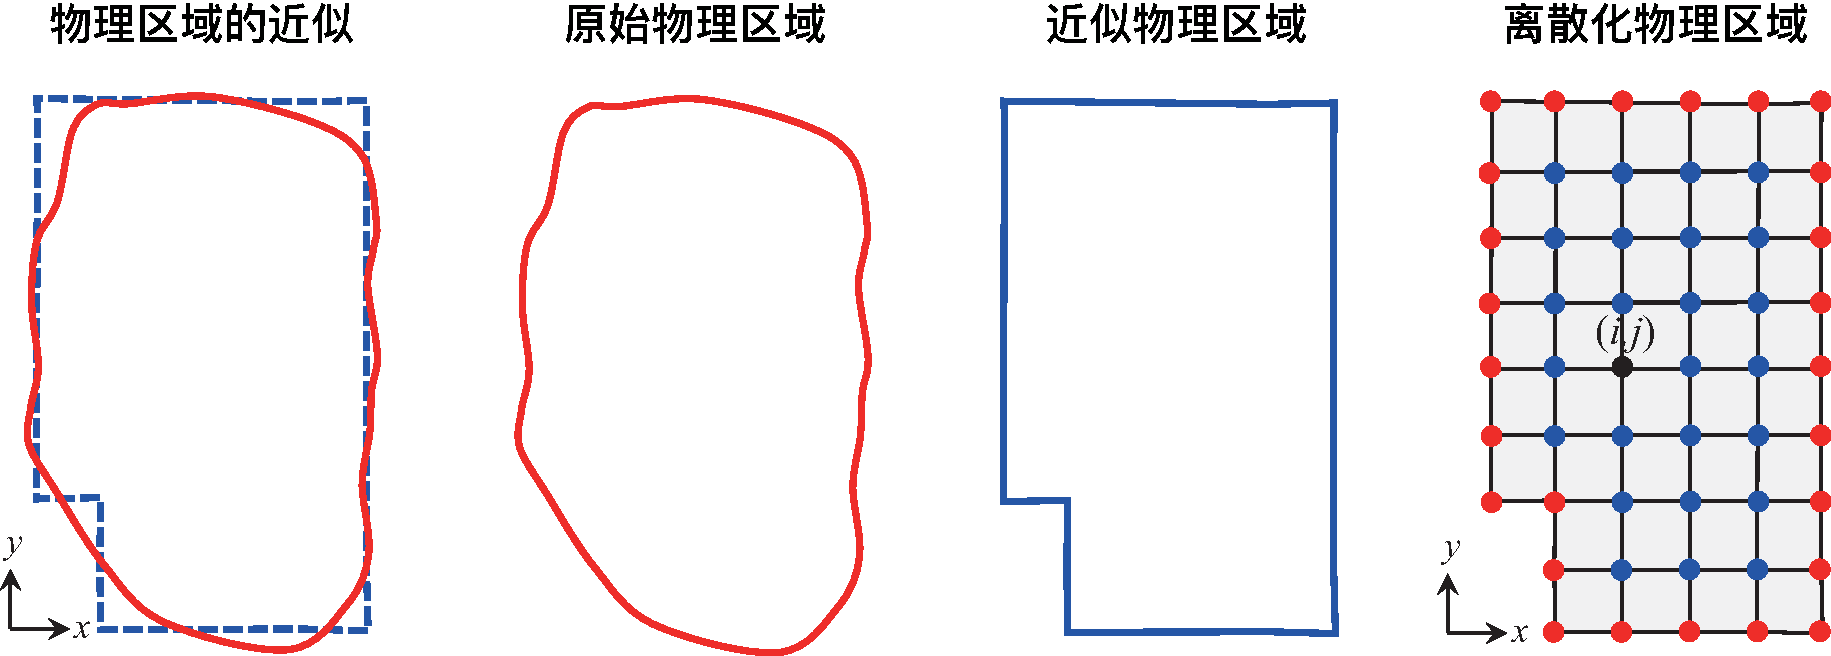
\includegraphics[width=0.85\linewidth]{pic/空间离散化.pdf}
	\caption{区域离散化}
	\label{区域离散化}
\end{figure}
	
离散化以后的区域,网格线的交点、以及网格线与边界的交点称为\dy[节点]{JD} ,用$( i,j)$标记其行和列的位置。红色为边界节点,蓝色为内部节点。正方形网格尺寸$h$称为\dy[节点间距]{JDJJ}。
\vspace*{0.5em}
	
\subsection{建立离散方程}
\begin{itemize}
	\item \textcolor{blue}{内部节点}(蓝色)需要建立离散方程\vspace*{-0.5em}
	\item \textcolor{red}{边界节点}(红色)需赋予相应的边界条件
\end{itemize}
\noindent \textbf{1. 边界条件的指定}

\begin{minipage}{0.7\linewidth}
	\vspace*{1em}
	\begin{itemize}
		\item 在原定解问题中,红色不规则边界上取值已知为$f(x,y)$
		\item 利用$f(x,y)$给定红色边界点上的值
		\item 利用\dy[最近点策略]{ZZDCL},即
		\begin{equation*}
			\mbox{任一红色边界节点的取值}\,=\,\mbox{原红色不规则区域上距离最近的点的取值}
		\end{equation*}
	\end{itemize}

\hspace*{-2em} \textbf{2. 内部节点离散方程的建立}
\vspace*{0.5em}

对于任一内部节点$(i,j)$,由二维Laplace方程可以得到离散方程
\end{minipage}
\begin{minipage}{0.25\linewidth}
	\centering
	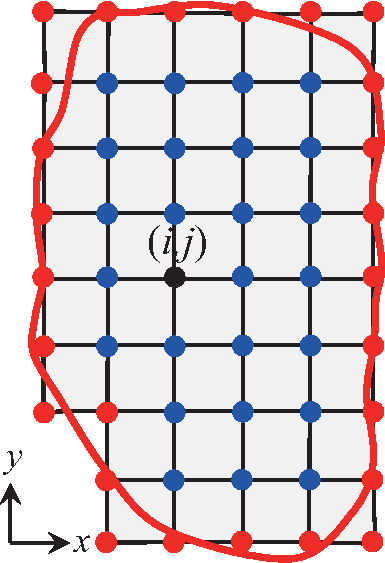
\includegraphics[width=0.8\linewidth]{pic/离散边界.pdf}
	\vspace*{-1em}
	\captionof{figure}{边界条件的指定}
\end{minipage}
\vspace*{0.5em}

\begin{equation}
	\dfrac{\partial^2 u}{\partial x^2} + \dfrac{\partial^2 u}{\partial y^2} \quad \Rightarrow \quad \dfrac{u_{i+1,j} - 2u_{i,j}+u_{i-1,j}}{h^2} + \dfrac{u_{i,j+1}-2u_{i,j}+u_{i,j-1}}{h^2} = 0
\end{equation}
化简得到
\begin{equation}
	u_{i+1,j} + u_{i-1,j} + u_{i,j+1} + u_{i,j-1} -4u_{i,j} = 0
	\label{离散方程}
\end{equation}
即\textcolor{red}{“四周相加,再减四倍”}。公式\eqref{离散方程}对内部所有节点都成立。
\vspace*{0.5em}

将所有离散方程联立得到一个\textbf{线性方程组}
\begin{equation}
	\bm{A}\bm{u}=\bm{B}
\end{equation}
其中,$\bm{A}$为系数矩阵,$\bm{u}$为内部节点未知量组成的列向量,非齐次项$\bm{B}$反映边界条件。
\vspace*{1em}

\noindent \textbf{3. 解线性方程组}

求解线性方程组有逆矩阵法和高斯消元法等成熟的算法,在Matlab里,求解$u$的方法为
\begin{center}
	\lstinline|u = A\B|
\end{center}

\examples \label{7.1}如图\ref{7.1.1}所示,给定矩形离散物理空间和边界条件,采用正方形网格,节点间距为$h =1$ ,求满足Laplace方程的内部节点。
\vspace*{-0.5em}
\begin{figure}[!htb]
	\begin{minipage}{0.5\linewidth}
		\centering
		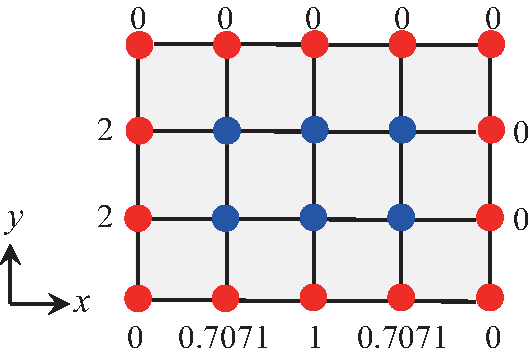
\includegraphics[width=0.6\linewidth]{pic/差分例1-1.pdf}
		\vspace*{-1em}
		\caption{\ref{7.1} $\,$题图}
		\label{7.1.1}
	\end{minipage}
	\begin{minipage}{0.5\linewidth}
		\centering
		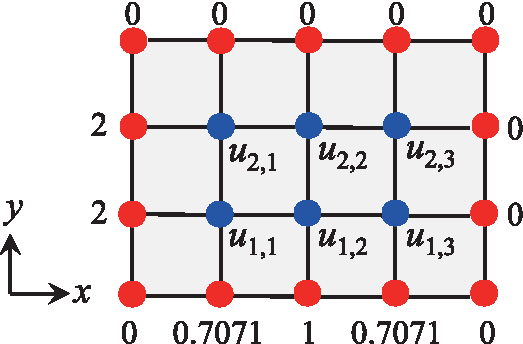
\includegraphics[width=0.6\linewidth]{pic/差分例1-2.pdf}
		\vspace*{-0.6em}
		\caption{\ref{7.1} $\,$编号图}
		\label{7.1.2}
	\end{minipage}
\end{figure}
\vspace*{-0.8em}

\solve 如图\ref{7.1.2}所示,将内部的节点编号,各个点的二阶中心差分离散方程为
\begin{align*}
	(1,1) \quad & u_{2,1} + 2 + 0.7071 + u_{1,2} -4u_{1,1}= 0\\
	(1,2) \quad & u_{2,2} + u_{1,1} + 1 + u_{1,2} -4u_{1,2}= 0\\
	(1,3) \quad & u_{2,3} + u_{1,2} + 0.7071 + 0 -4u_{1,3}= 0\\
	(2,1) \quad & 0 + 2 + u_{1,1} + u_{2,2} -4u_{2,1}= 0\\
	(2,2) \quad & 0 + u_{2,1} + u_{1,2} + u_{2,3} -4u_{2,2}= 0\\
	(2,3) \quad & 0 + u_{2,2} + u_{1,3} + 0 -4u_{2,3}= 0
\end{align*}
得到线性方程组
\begin{equation*}
	\begin{bmatrix}
		-4 & 1 & 0 & 1 & 0 & 0\\
		1& -4 & 1 &  0 & 1 & 0 \\
		0& 1 & -4&  0& 0 & 1\\
		1& 0 & 0 & -4 & 1 & 0\\
		0 & 1 & 0  & 1 & -4 & 1\\
		0& 0& 1 &0 & 0 &-4
	\end{bmatrix}
	\,\,
	\begin{bmatrix}
		u_{1,1}\\
		u_{1,2}\\
		u_{1,3}\\
		u_{2,1}\\
		u_{2,2}\\
		u_{2,3}
	\end{bmatrix}
	\,\,
	=
	\,\,
	\begin{bmatrix}
		-2.7071\\
		-1\\
		-0.7071\\
		-2\\
		0\\
		0
	\end{bmatrix}
\end{equation*}
利用Matlab解得
\begin{equation*}
	\begin{bmatrix}
		u_{1,1}\\
		u_{1,2}\\
		u_{1,3}\\
		u_{2,1}\\
		u_{2,2}\\
		u_{2,3}
	\end{bmatrix}
	\, = \,
	\begin{bmatrix}
		1.0835\\
		0.7405\\
		0.4186\\
		0.8863\\
		0.4616\\
		0.2196
	\end{bmatrix}
\end{equation*}
\vspace*{1em}

\subsection{$\mbox{第三类边界条件的处理}^*$}
上一节仅考虑了第一类边界条件,对于更一般的第三类边界条件的处理如下。
\begin{figure}[!htb]
	\centering
	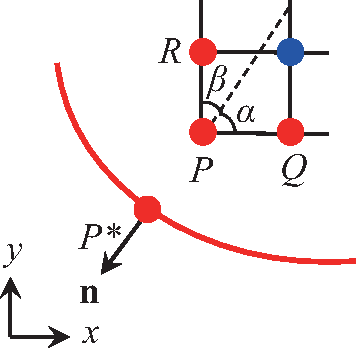
\includegraphics[width=0.2\linewidth]{pic/离散第三边界.pdf}
	\caption{第三边界条件下的边界差分方程}
	\label{第三边界差分}
\end{figure}

如图\ref{第三边界差分},考虑边界上一点$P$,其邻近点记作$Q$和$R$,正方形网格尺寸为$h$,$P$点在真实物理区域上的最近点记作$P^*$.

\noindent 由第三类边界条件,在$P^*$点满足
\begin{equation}
	u(P^*) + \sigma \dfrac{\partial u}{\partial n}\Bigg|_{P^*} = f(P^*)
\end{equation}

\noindent 由最近点方案,可得
\begin{equation}
	u(P) + \sigma \dfrac{\partial u}{\partial n}\Bigg|_{P} = f(P) = f(P^*)
\end{equation}

\noindent 根据几何关系
\begin{equation}
	\dfrac{\partial u}{\partial n}\Bigg|_{P} = - \left(\dfrac{\partial u}{\partial x}\Bigg|_{P} \cos \alpha + \dfrac{\partial u}{\partial y}\Bigg|_{P} \sin \alpha\right)
\end{equation}

\noindent 综合可得
\begin{equation}
	u(P) - \sigma \dfrac{\partial u}{\partial x}\Bigg|_{P}\cos \alpha - \sigma \dfrac{\partial u}{\partial y}\Bigg|_{P} \sin \alpha = f(P^*)
\end{equation}

\noindent 由前向差分的定义
\begin{equation}
	\dfrac{\partial u}{\partial x}\Bigg|_{P} = \dfrac{u(Q) - u(P)}{h}, \quad \dfrac{\partial u}{\partial y}\Bigg|_{P} = \dfrac{u(R) - u(P)}{h}
\end{equation}

\noindent 最终整理得到
\begin{equation}
	[h+\sigma \cos \alpha + \sigma \sin \alpha ]u(P) - (\sigma \cos \alpha)u(Q)-(\sigma \sin \alpha)u(R) = f(P^*)h
	\label{离散第三边界}
\end{equation}

公式\eqref{离散第三边界}仅为\textbf{边界节点值的代数方程},仍需和和内部节点公式\eqref{离散方程}联合组成线性方程组,一并求解。
\vspace*{1em}

\subsection{总结}
 Laplace方程的差分解法总结如下
\begin{enumerate}
	\item \textbf{用一系列离散节点$(i,j)$代替原物理域}
	\item \textbf{处理边界方程,得到离散方程}
	\begin{itemize}
		\item \textbf{第一类边界条件}\quad 对每一内部节点,选取适当的差分格式,得到其离散方程,组成线性方程组
		\item \textbf{第二、第三类边界条件 }\quad 边界条件满足的离散方程将额外给出,和内部节点的方程联立得到线性方程组,其方程数量更多
	\end{itemize}
	\item \textbf{求解线性方程组},得到未知节点处的解,即为原定解问题的近似解。
\end{enumerate}

\warn[
{
\begin{enumerate}
	\item \textbf{网格的形状可以是任意的}\\
	\hspace*{2em}网格不一定是正方形,可以是矩形、平行四边形、三角形、正六边形等等
	\item \textbf{差分格式是多样的}\\
	\hspace*{2em}对于一阶导数,本节介绍了前向、后向、中心差分,对于二阶导数,只介绍了中心差分,然而实际上还有更多更复杂的、精度更高的差分格式
	\item \textbf{线性方程组的求解方法也多种多样}
	\item \textbf{方程还可以含有非齐次项,差分法中称为\dy[源项]{YX}。}所以,这里仅讨论了最简单、最基本的情况。\\[-1em]
\end{enumerate}
}
]
\clearpage

\section{热传导方程的差分解法}
考虑一维热传导方程的简单情况:分析长度为1的杆在$0 \sim T$之间的温度变化,其初始温度为$f(x)$,两端温度固定为0,即
\begin{equation}
	\begin{cases}
		\, \dfrac{\partial u}{\partial t} = a^2 \dfrac{\partial^2 u}{\partial x^2}, & 0<x<1,0<t\le T\\[0.5em]
		\, u\big|_{t=0} = f(x), & 0 \le x \le 1\\
		\, u\big|_{x=0} = u\big|_{x=1} = 0, & 0 < t \le T
	\end{cases}
\end{equation}
\vspace*{0.5em}

\subsection{时间变量的特殊性}
\begin{enumerate}[1. ]
	\item 热传导方程与Laplace方程的不同之处在于,热传导方程是一个\textcolor{red}{非稳态过程},即结果随时间变化的过程。\vspace*{-0.5em}
	\item 非稳态过程的特点是\textcolor{blue}{后一时刻的状态依赖于前一状态},即不能同时知道所有时刻的状态。时间变量必须从$0\sim T$,每一步时间的增量称为\dy[时间步长]{SJBC},记作$\Delta t$.\vspace*{-0.5em}
	\item 求解的过程可以理解为\textcolor{blue}{“基于过去,预测未来”}(随时间向前迭代),其精度与$\Delta t$的长度(步长)相关。
\end{enumerate}

\subsection{建立离散方程}
设空间离散点在某一时刻的状态为$u_i^n$,其中下标$i$表示空间信息,上标$n$表示时间信息。在这里离散成6个等间距节点,其中4 个内部节点,2个边界节点,记节点间距为$h$.如图\ref{一维差分传热}所示。
\begin{figure}[!htb]
	\centering
	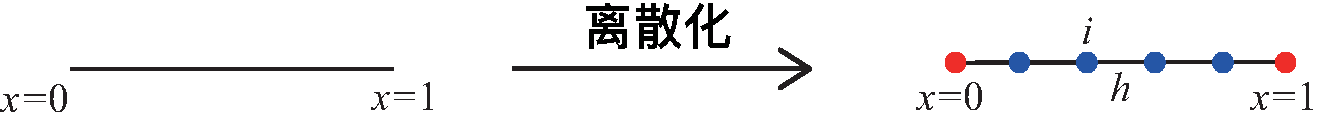
\includegraphics[width=0.6\linewidth]{pic/一维差分传热.pdf}
	\caption{一维传热计算域离散化}
	\label{一维差分传热}
\end{figure}

\noindent \textbf{1. 考虑时间导数项}
\begin{equation*}
	\boxed{\dfrac{\partial u}{\partial t}} = a^2 \dfrac{\partial^2 u}{\partial x^2}
\end{equation*}
\begin{itemize}
	\item 时间导数的差分格式必须要用到下一步的时间信息,才能实现时间推进。由\ptref[差分的四种表示形式]可知只有前向差分和中心差分满足要求。
	\item 这里采用较为简单的前向差分。对目前处于第$n$个时刻的第$i$个内部节点,时间导数项差分后
	\begin{equation}
		\dfrac{u_i^{n+1}-u_i^n}{\Delta t} = a^2 \dfrac{\partial^2 u}{\partial x^2}\Bigg|_i
	\end{equation}
\end{itemize}
\noindent \textbf{2. 考虑空间导数项}
\begin{equation*}
	\dfrac{u_i^{n+1}-u_i^n}{\Delta t} = a^2\,\, \boxed{\dfrac{\partial^2 u}{\partial x^2}\Bigg|_i}
\end{equation*}
\begin{enumerate}[\hspace*{2em} (1) ]
	\item \textbf{显式格式}\\
	当空间导数项采用$n$时刻的空间数据(已知的数据)时,此时可以得到显式方程
	\begin{equation}
		\dfrac{u_i^{n+1}-u_i^n}{\Delta t} = a^2 \dfrac{u_{i+1}^n - 2u_i^n + u_{i-1}^n}{h^2}
	\end{equation}
	从而得到各点的离散方程
	\begin{align*}
		(n,1)\quad &\dfrac{u_1^{n+1}-u_1^n}{\Delta t} = a^2 \dfrac{u_{2}^n - 2u_1^n }{h^2}\\[0.5em]
		(n,2)\quad &\dfrac{u_2^{n+1}-u_2^n}{\Delta t} = a^2 \dfrac{u_{3}^n - 2u_2^n + u_1^n}{h^2}\\[0.5em]
		(n,3)\quad &\dfrac{u_3^{n+1}-u_3^n}{\Delta t} = a^2 \dfrac{u_{4}^n - 2u_3^n + u_2^n}{h^2}\\[0.5em]
		(n,4)\quad &\dfrac{u_1^{n+1}-u_1^n}{\Delta t} = a^2 \dfrac{- 2u_4^n + u_3^n}{h^2}
	\end{align*}
	整理得
	\begin{align}
		\bm{u}^{n+1} = \bm{B}^n
	\end{align}
	其中,
	\begin{equation}
		\bm{u}^{n+1} = 
		\begin{bmatrix}
			\, u_1^{n+1}\, \\
			\, u_2^{n+1}\, \\
			\, u_3^{n+1}\, \\
			\, u_4^{n+1}\,
		\end{bmatrix}
	\quad \quad
	\bm{B}^n = 
	\begin{bmatrix}
		\, u_1^n + a^2 \dfrac{u_{2}^n - 2u_1^n }{h^2}\Delta t \,\\[1em]
		\, u_2^n + a^2 \dfrac{u_{3}^n - 2u_2^n + u_1^n}{h^2} \Delta t \, \\[1em]
		\, u_3^n+a^2 \dfrac{u_{4}^n - 2u_3^n + u_2^n}{h^2}\Delta t \, \\[1em]
		\, u_4^n +a^2 \dfrac{- 2u_4^n + u_3^n}{h^2} \Delta t \, 
	\end{bmatrix}
	\end{equation}
	\vspace*{0.5em}
	
	\item \textbf{隐式格式}\\
	当空间导数项采用$n+1$时刻的空间数据(未知的数据)时,此时可以得到隐式方程
	\begin{equation}
		\dfrac{u_i^{n+1}-u_i^n}{\Delta t} = a^2 \dfrac{u_{i+1}^{n+1} - 2u_i^{n+1} + u_{i-1}^{n+1}}{h^2}
	\end{equation}
	从而得到各点的离散方程
	\begin{align*}
		(n+1,1)\quad &\dfrac{u_1^{n+1}-u_1^n}{\Delta t} = a^2 \dfrac{u_{2}^{n+1} - 2u_1^{n+1} }{h^2}\\[0.5em]
		(n+1,2)\quad &\dfrac{u_2^{n+1}-u_2^n}{\Delta t} = a^2 \dfrac{u_{3}^{n+1} - 2u_2^{n+1} + u_1^{n+1}}{h^2}\\[0.5em]
		(n+1,3)\quad &\dfrac{u_3^{n+1}-u_3^n}{\Delta t} = a^2 \dfrac{u_{4}^{n+1} - 2u_3^{n+1} + u_2^{n+1}}{h^2}\\[0.5em]
		(n+1,4)\quad &\dfrac{u_1^{n+1}-u_1^n}{\Delta t} = a^2 \dfrac{- 2u_4^{n+1} + u_3^{n+1}}{h^2}
	\end{align*}
	整理得
	\begin{align}
		\bm{A}\bm{u}^{n+1} = \bm{B}^n
	\end{align}
	其中,
	\begin{equation}
		\bm{u}^{n+1} = 
		\begin{bmatrix}
			\, u_1^{n+1}\, \\
			\, u_2^{n+1}\, \\
			\, u_3^{n+1}\, \\
			\, u_4^{n+1}\,
		\end{bmatrix}
		\quad \quad
		\bm{B}^n = 
		\begin{bmatrix}
			\, u_1^{n}\, \\
			\, u_2^{n}\, \\
			\, u_3^{n}\, \\
			\, u_4^{n}\,
		\end{bmatrix}
		\quad \quad 
		\bm{A} =
		\begin{bmatrix}
			\, 1+\dfrac{2a^2}{h^2}\Delta t & -\dfrac{a^2}{h^2}\Delta t & 0 & 0\,\, \\[1em]
			\, -\dfrac{a^2}{h^2} \Delta t & 1+\dfrac{2a^2}{h^2}\Delta t & -\dfrac{a^2}{h^2}\Delta t & 0 \,\, \\[1em]
			\, 0 & -\dfrac{a^2}{h^2}\Delta t  & 1+\dfrac{2a^2}{h^2}\Delta t & -\dfrac{a^2}{h^2}\Delta t \,\, \\[1em]
			\, 0 & 0 & -\dfrac{a^2}{h^2}\Delta t  &1+\dfrac{2a^2}{h^2}\Delta t \,\,
		\end{bmatrix}
	\end{equation}
\end{enumerate}
\subsection{时间推进}
\noindent \textbf{1. 显式格式的时间推进}
\begin{figure}[!htb]
	\centering
	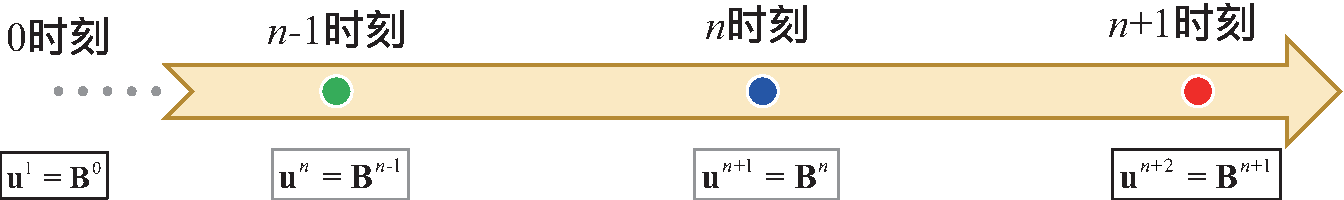
\includegraphics[width=0.7\linewidth]{pic/显式时间.pdf}
	\caption{显式格式的时间推进}
\end{figure}
\vspace*{-2em}

\begin{itemize}
	\item $n$从0开始递增,直到$t=T$为止。
	\item 在每一时刻,只需进行代数运算获得$\bm{B}^n$便得$\bm{u}^{n+1}$,计算量小。
	\item 然而,\textcolor{red}{显式格式的时间步长要很小},否则很容易出现解振荡发散的现象。
\end{itemize}
\vspace*{1em}

\noindent \textbf{2. 隐式格式的时间推进}
\begin{figure}[!htb]
	\centering
	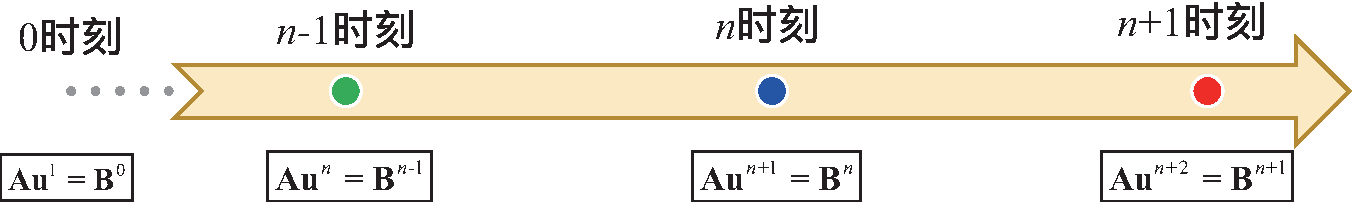
\includegraphics[width=0.7\linewidth]{pic/隐式时间.pdf}
	\caption{隐式格式的时间推进}
\end{figure}
\vspace*{-2em}

\begin{itemize}
	\item $n$从0开始递增,直到$t=T$为止。
	\item 在每一时刻,需求解线性方程组,计算量较大。
	\item 与此同时,\textcolor{red}{允许时间更大的时间步长}。
\end{itemize}

\examples \label{7.2} 考虑长为4的一维杆的热传导问题。已将杆离散为5个节点构成的网格,节点间距$h=1$,内节点标记为$u_1,u_2,u_3$.杆的初始温度和边界温度固定为0,如图\ref{7.2.1}所示。已知热扩散系数$a_2=1$,取时间步长$\Delta t=0.1$,用显式差分法求$t=0.2$时的温度场近似解。
\begin{figure}[!htb]
	\centering
	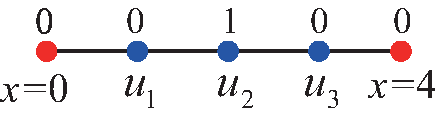
\includegraphics[width=0.24\linewidth]{pic/7.2.1.pdf}
	\vspace*{-0.8em}
	\caption{\ref{7.2}$\,$题图}
	\label{7.2.1}
\end{figure}
\vspace*{-1.5em}

\solve 根据显式有限差分,将方程离散为
\begin{equation*}
	\dfrac{u_i^{n+1}-u_i^n}{\Delta t} = a^2 \dfrac{u_{i+1}^{n+1} - 2u_i^{n+1} + u_{i-1}^{n+1}}{h^2}
	\quad \Rightarrow \quad
	u_i^{n+1} = u_i^n + 0.1\big(u_{i+1}^n -2u_i^n + u_{i-1}^n\big)
\end{equation*}
然后进行时间推进,即将$n=0,\,\,i=1,2,3$代入,得到$t=0.1$时刻的节点值满足
\begin{equation*}
	\begin{aligned}
		u_1^1 &= u_1^0 + 0.1\big(u_2^0 - 2u_1^0 + u_0^0\big)\\
		u_2^1 &= u_2^0 + 0.1\big(u_3^0 - 2u_2^0 +u_1^0\big)\\
		u_3^1 &= u_3^0 + 0.1\big(u_4^0 - 2u_3^0 + u_2^0\big)
	\end{aligned}
	\quad \quad \xrightarrow[\mbox{边界条件}]{\quad \mbox{代入初始条件} \quad} \quad \quad 
	\begin{aligned}
		u_1^1 &= 0+0.1(1-0+0)=0.1\\
		u_2^1 &= 1+0.1(0-2+0)=0.8\\
		u_3^1 &= 0 + 0.1(0-0+1)=0.1
	\end{aligned}
\end{equation*}
得到$t=0.1$时刻的节点值如图\ref{7.2.2}.
\begin{figure}[!htb]
	\centering
	\begin{minipage}{0.4\linewidth}
		\centering
		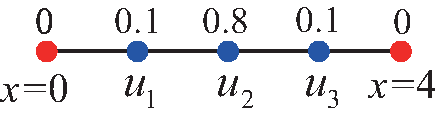
\includegraphics[width=0.6\linewidth]{pic/7.2.2.pdf}
		\vspace*{-0.8em}
		\caption{$t=0.1$时刻的节点值}
		\label{7.2.2}
	\end{minipage}
	\begin{minipage}{0.4\linewidth}
		\centering
		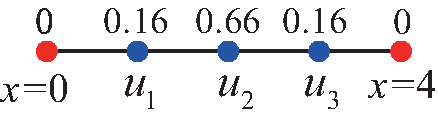
\includegraphics[width=0.6\linewidth]{pic/7.2.3.pdf}
		\vspace*{-0.5em}
		\caption{$t=0.2$时刻的节点值}
		\label{7.2.3}
	\end{minipage}
\end{figure}

继续将$n=1,\,\,i=1,2,3$代入,得到$t=0.2$时刻的节点值满足
\begin{equation*}
	\begin{aligned}
		u_1^2 &= u_1^1 + 0.1\big(u_2^1 - 2u_1^1 + u_0^1\big)\\
		u_2^2 &= u_2^1 + 0.1\big(u_3^1 - 2u_2^1 +u_1^1\big)\\
		u_3^2 &= u_3^1 + 0.1\big(u_4^1 - 2u_3^1 + u_2^1\big)
	\end{aligned}
	\quad \quad \xrightarrow[\mbox{边界条件}]{\quad \mbox{代入新的初始条件} \quad} \quad \quad 
	\begin{aligned}
		u_1^2 &= 0.1+0.1(0.8-2\times 0.1 +0)=0.16\\
		u_2^2 &= 0.8+0.1(0-2\times 0.8+0.1)=0.66\\
		u_3^2 &= 0.1 + 0.1(0-2\times 0.1+0.8)=0.16
	\end{aligned}
\end{equation*}
得到$t=0.2$时刻的节点值如图\ref{7.2.3}.
\vspace*{0.5em}

\subsection{总结}
总结如图\ref{非稳态热传导差分解法总结}所示。
\begin{figure}[!htb]
	\centering
	\begin{tikzpicture}
		\node (A) [inner sep = 6pt, draw] {\makecell[c]{热传导方程同时含有\textcolor{blue}{时间导数}和\textcolor{blue}{空间导数},\\
		由非稳态问题的特点,求解需采用\textcolor{red}{时间推进策略}}};
		\node (B) [inner sep =6pt, draw, below of = A, node distance = 3cm, xshift = -4cm]{\textcolor{blue}{时间导数项$\dfrac{\partial u}{\partial t}$}};
		\node (B1) [inner sep =6pt, draw, below of = B, node distance = 2cm]{时间变量的特殊性:\textcolor{red}{向前不向后}};
		\node (B2) [inner sep = 6pt, draw, below of = B1, node distance = 2.5cm]{$\dfrac{u_i^{n+1}-u_i^n}{\Delta t} = a^2 \dfrac{\partial^2 u}{\partial x^2}\Bigg|_i$};
		
		\node (C) [inner sep =6pt, draw, below of = A, node distance = 3cm, xshift = 4cm]{\textcolor{blue}{空间导数项$\dfrac{\partial^2 u}{\partial x^2}\Bigg|_i$}};
		\node (C1) [inner sep =6pt, draw, below of = C, node distance = 2cm]{采用二阶中心差分,考虑\textcolor{red}{时间的选取}};
		\node (C11) [inner sep =6pt, draw, below of = C1, node distance = 2.2cm, xshift = -2.5cm]{显式格式};
		\node (C111) [inner sep =6pt, draw, below of = C11, node distance = 1.5cm]{$\bm{u}^{n+1} = \bm{B}^n$};
		\node (C112) [inner sep =6pt, draw, below of = C111, node distance = 2cm]{\makecell[c]{每一时间步计算量小,\\
		但要求时间步长相对较小}};
		\node (C12) [inner sep =6pt, draw, below of = C1, node distance = 2.2cm, xshift = 2.5cm]{隐式格式};
		\node (C121) [inner sep =6pt, draw, below of = C12, node distance = 1.5cm]{$\bm{A}\bm{u}^{n+1} = \bm{B}^n$};
		\node (C122) [inner sep =6pt, draw, below of = C121, node distance = 2cm]{\makecell[c]{每一时间步计算量大,\\
			但时间步长可以相对较大}};
		
		\node (D) [inner sep =6pt, draw, below of = A, node distance = 13.5cm, xshift = 0.5cm]{计算从初始时刻不断推进,直到达到想要的时刻,停止计算};
		
		\draw [arrows={-Stealth}] (A) --+(0cm, -1.5cm) -- +(-4cm, -1.5cm) -- (B);
		\draw [arrows={-Stealth}] (A) --+(0cm, -1.5cm) -- +(4cm, -1.5cm) -- (C);
		\draw [arrows={-Stealth}] (B) -- (B1);
		\draw [arrows={-Stealth}]  (C) -- (C1);
		\draw [arrows={-Stealth}]  (B1) -- (B2)node[midway, xshift = -1cm]{前向差分};
		\draw [arrows={-Stealth}]  (C1) --+(0cm,-1.4cm) --+(-2.5cm, -1.4cm)node[near end, above = 0.5mm, xshift = -5mm]{{\small 选取\textcolor{blue}{已知时刻}的变量}} -- (C11);
		\draw [arrows={-Stealth}]  (C1) --+(0cm,-1.4cm) --+(2.5cm, -1.4cm)node[near start, above = 0.5mm, xshift = +18mm]{{\small 选取\textcolor{blue}{待求时刻}的变量}} -- (C12);
		\draw  (C11) -- (C111);
		\draw (C111) -- (C112);
		\draw  (C12) -- (C121);
		\draw (C121) -- (C122);
		\draw [arrows={-Stealth}] (B2) -- (-4cm,-12.5cm) -- (0.5cm,-12.5cm) -- (D);
		\draw [arrows={-Stealth}] (C112) -- (1.5cm, -12cm) -- (4cm, -12cm) -- (4cm, -12.5cm);
		\draw [arrows={-Stealth}] (C122) -- (6.5cm, -12cm) -- (4cm, -12cm) -- (4cm, -12.5cm);
		\draw(4cm, -12.5cm) -- (0.5cm,-12.5cm);
	\end{tikzpicture}
	\caption{非稳态热传导差分解法总结}
	\label{非稳态热传导差分解法总结}
\end{figure}

\clearpage
\vspace*{-3em}

\warn[
\hspace*{1em} 1. \textbf{时间步长}和\textbf{网格尺寸}越小,计算越精确,但计算量也越大\vspace*{0.5em}\\
\hspace*{1em} 2. 对于热传导方程,当\textbf{时间推进到足够大}时,过程不再随时间变化,此时得到的是\textbf{对应的Laplace方程的解}。
]


\section{波动方程的差分解法}
考虑一维波动方程的简单情况:分析长度为1的两端固定弦在$0\sim T$时刻之间的振动过程,初位移为$\varphi(x)$,初速度为$\psi(x)$.即
\begin{equation}
	\begin{cases}
		\, \dfrac{\partial^2 u}{\partial t^2} = a^2 \dfrac{\partial^2 u}{\partial x^2}, & 0<x<1,0<t\le T\\[0.5em]
		\, u\big|_{t=0} = \varphi(x), \,\,\dfrac{\partial u}{\partial t}\Bigg|_{t=0} = \psi(x), & 0 \le x \le 1\\[0.5em]
		\, u\big|_{x=0} = u\big|_{x=1} = 0, & 0 < t \le T
	\end{cases}
\end{equation}
不难发现,波动方程与热传导方程相比,时间导数变为二阶导数,因此差分求解的思路很相似。
\vspace*{0.5em}

\subsection{求解步骤}
\begin{enumerate}[\textbf{步骤} 1 ]
	\item \textbf{区域离散化}\\
	设空间离散点在某一时刻的状态为$u_i^n$,其中下标$i$表示空间信息,上标$n$表示时间信息。在这里离散成6个等间距节点,其中4 个内部节点,2个边界节点,记节点间距为$h$.如图\ref{一维差分波动}所示。
	\begin{figure}[!htb]
		\centering
		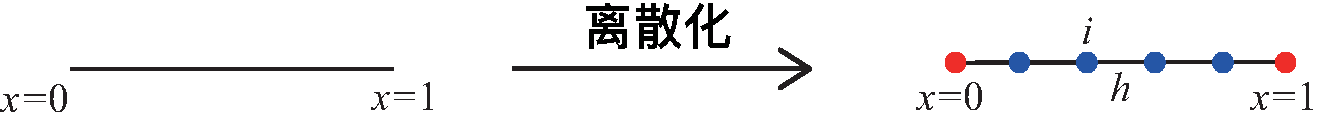
\includegraphics[width=0.6\linewidth]{pic/一维差分传热.pdf}
		\caption{一维波动计算域离散化}
		\label{一维差分波动}
	\end{figure}
	
	\item \textbf{建立离散方程}
	\begin{enumerate}[(1) ]
		\item \textbf{时间导数项}\\
		\hspace*{1em} 对目前处于第$n$个时刻的第$i$个内部节点,时间导数项二阶中心差分
		\begin{equation}
			\dfrac{u_i^{n+1}-2u_i^n+u_i^{n-1}}{(\Delta t)^2} = a^2 \dfrac{\partial^2 u}{\partial x^2}\Bigg|_i
			\label{一维波动差分时间}
		\end{equation}
		显然,当$n=0$时不存在第$-1$时刻的值,所以公式\eqref{一维波动差分时间}需要满足$n \ge 1$。所以,对于第一步的时间推进$n = 0$需要考虑初始条件所引入的差分,即二阶中心差分的另一种表示方式:
		\begin{equation}
			\dfrac{\left(\dfrac{\partial u}{\partial t}\right)^1 - \left(\dfrac{\partial u}{\partial t}\right)^0}{\Delta t} = a^2 \dfrac{\partial^2 u}{\partial x^2}\Bigg|_i 
			\quad \Rightarrow \quad
			\dfrac{\dfrac{u_1^1-u_1^0}{\Delta t} - \psi(x_i)}{\Delta t}= a^2 \dfrac{\partial^2 u}{\partial x^2}\Bigg|_i 
		\end{equation}
		可以得到第一步时间推进最终的解
		\begin{equation}
			u_i^1=\varphi(x_i)+\psi(x_i)\Delta t + a^2 (\Delta t)^2\dfrac{\partial^2 u}{\partial x^2}\Bigg|_i
		\end{equation}
		\clearpage
		
		\item \textbf{空间导数项}
		\begin{enumerate}[i. ]
			\item \textbf{显式格式}\\
			选取已知的$n$时刻
			\begin{equation}
				\begin{cases}
					\, u_i^1=\varphi(x_i)+\psi(x_i)\Delta t + a^2 (\Delta t)^2\dfrac{\varphi(x_{i+1})-2\varphi(x_i)+\varphi(x_{i-1})}{h^2}, & n = 0\\[1em]
					\,
					\dfrac{u_i^{n+1}-2u_i^n+u_i^{n-1}}{(\Delta t)^2} = a^2 \dfrac{u_{i+1}^n - 2u_i^n + u_{i-1}^n}{h^2}, & n \ge 1
				\end{cases}
			\end{equation}
			整理得
			\begin{equation}
				\bm{u}^{n+1} = \bm{B}^n
			\end{equation}
			其中,
			\begin{align}
				\bm{u}^{n+1} = 
			\begin{bmatrix}
				\, u_1^{n+1}\, \\
				\, u_2^{n+1}\, \\
				\, u_3^{n+1}\, \\
				\, u_4^{n+1}\,
			\end{bmatrix}
			\quad \quad
			\bm{B}^0 &= 
			\begin{bmatrix}
				\, \varphi(x_1)+\psi(x_1)\Delta t + a^2 (\Delta t)^2\dfrac{\varphi(x_2)-2\varphi(x_1)}{h^2} \,\\[1em]
				\, \varphi(x_2)+\psi(x_2)\Delta t + a^2 (\Delta t)^2\dfrac{\varphi(x_3)-2\varphi(x_2) + \varphi(x_1)}{h^2} \, \\[1em]
				\,  \varphi(x_3)+\psi(x_3)\Delta t + a^2 (\Delta t)^2\dfrac{\varphi(x_4)-2\varphi(x_3) + \varphi(x_2)}{h^2}  \, \\[1em]
				\, \varphi(x_4)+\psi(x_4)\Delta t + a^2 (\Delta t)^2\dfrac{-2\varphi(x_4) + \varphi(x_3)}{h^2} \, 
			\end{bmatrix}
			\\[1em]
			\bm{B}^{n}(n\ge 1)& =
			\begin{bmatrix}
				\, 2u_1^n - u_1^{n-1} + a^2(\Delta t)^2\dfrac{u_2^n-2u_1^n}{h^2}\,\\[1em]
				\,2u_2^n - u_2^{n-1} + a^2(\Delta t)^2\dfrac{u_3^n-2u_2^n+u_1^n}{h^2} \, \\[1em]
				\,  2u_3^n - u_3^{n-1} + a^2(\Delta t)^2\dfrac{u_4^n-2u_3^n + u_2^n}{h^2}  \, \\[1em]
				\, 2u_4^n - u_4^{n-1} + a^2(\Delta t)^2\dfrac{-2u_4^n+u_3^n}{h^2} \, 
			\end{bmatrix}
			\end{align}
			
			\item \textbf{隐式格式}\\
			选取待求的$n+1$时刻
			\begin{equation}
				\begin{cases}
					\, u_i^1=\varphi(x_i)+\psi(x_i)\Delta t + a^2 (\Delta t)^2\dfrac{u_{i+1}^1-2u_i^1+u_{i-1}^1}{h^2}, & n = 0\\[1em]
					\,
					\dfrac{u_i^{n+1}-2u_i^n+u_i^{n-1}}{(\Delta t)^2} = a^2 \dfrac{u_{i+1}^{n+1} - 2u_i^{n+1} + u_{i-1}^{n+1}}{h^2}, & n \ge 1
				\end{cases}
			\end{equation}
			其中,
			\begin{align}
				\bm{u}^{n+1} = 
				\begin{bmatrix}
					\, u_1^{n+1}\, \\
					\, u_2^{n+1}\, \\
					\, u_3^{n+1}\, \\
					\, u_4^{n+1}\,
				\end{bmatrix}
				\quad \quad 
				&\bm{A} =
				\begin{bmatrix}
					\, 1+\dfrac{2a^2}{h^2}(\Delta t)^2 & -\dfrac{a^2}{h^2}(\Delta t)^2 & 0 & 0\,\, \\[1em]
					\, -\dfrac{a^2}{h^2}(\Delta t)^2 & 1+\dfrac{2a^2}{h^2}(\Delta t)^2 & -\dfrac{a^2}{h^2}(\Delta t)^2 & 0 \,\, \\[1em]
					\, 0 & -\dfrac{a^2}{h^2}(\Delta t)^2 & 1+\dfrac{2a^2}{h^2}(\Delta t)^2 & -\dfrac{a^2}{h^2}(\Delta t)^2 \,\, \\[1em]
					\, 0 & 0 & -\dfrac{a^2}{h^2}(\Delta t)^2 & 1+\dfrac{2a^2}{h^2}(\Delta t)^2 \,\,
				\end{bmatrix}\\[1em]
				\bm{B}^0 &= 
				\begin{bmatrix}
					\, \varphi(x_1)+\psi(x_1)\Delta t  \,\\
					\, \varphi(x_2)+\psi(x_2)\Delta t \, \\
					\,  \varphi(x_3)+\psi(x_3)\Delta t \, \\
					\, \varphi(x_4)+\psi(x_4)\Delta t \, 
				\end{bmatrix}
				\quad \quad 
				\bm{B}^n(n\ge 1) = 
				\begin{bmatrix}
					\, 2u_1^n - u_1^{n-1} \,\\
					\,2u_2^n - u_2^{n-1} \, \\
					\,  2u_3^n - u_3^{n-1}   \, \\
					\, 2u_4^n - u_4^{n-1}  \, 
				\end{bmatrix}
			\end{align}
		\end{enumerate}
	\end{enumerate}
	\item \textbf{时间推进}
	\begin{enumerate}[(1) ]
		\item \textbf{显式格式}
		\begin{figure}[!htb]
			\centering
			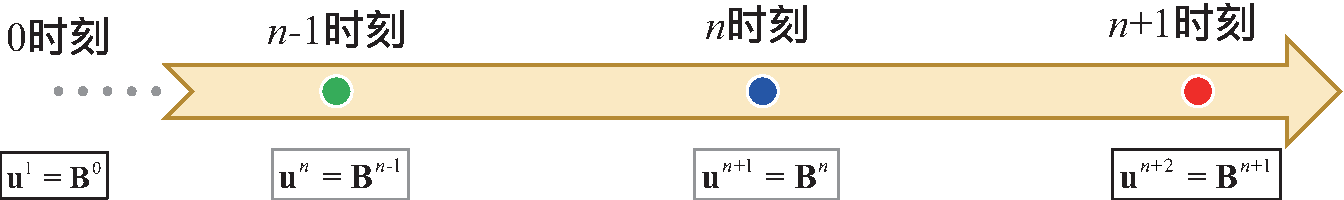
\includegraphics[width=0.7\linewidth]{pic/显式时间.pdf}
			\caption{显式格式的时间推进}
		\end{figure}
		\vspace*{-1em}
		
		\begin{itemize}
			\item $n$从0开始递增,直到$t=T$为止。
			\item 在每一时刻,只需进行代数运算获得$\bm{B}^n$便得$\bm{u}^{n+1}$,计算量小。
			\item 然而,\textcolor{red}{显式格式的时间步长要很小},否则很容易出现解振荡发散的现象。
		\end{itemize}
	
	\item \textbf{隐式格式}
	\begin{figure}[!htb]
		\centering
		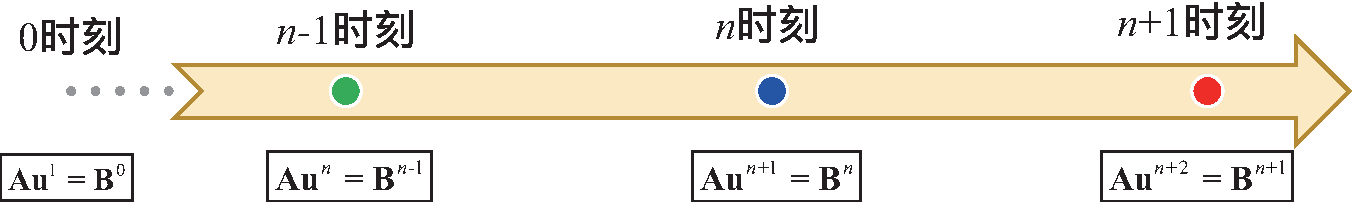
\includegraphics[width=0.7\linewidth]{pic/隐式时间.pdf}
		\caption{隐式格式的时间推进}
	\end{figure}
	\vspace*{-1em}
	
	\begin{itemize}
		\item $n$从0开始递增,直到$t=T$为止。
		\item 在每一时刻,需求解线性方程组,计算量较大。
		\item 与此同时,\textcolor{red}{允许时间更大的时间步长}。
	\end{itemize}
	\end{enumerate}
\end{enumerate}
\warn[
{
\begin{enumerate}
	\item 整体看来,与热传导方程的差分求解方法很像。
	\item 由于时间导数项变成二阶了,因此在采用二阶时间导数的中心差分时,\textcolor{red}{需要单独处理第一步时间迭代$n=0$}。
	\item 在热传导方程的求解中需要注意的事项,在这里同样需要注意。
\end{enumerate}
}
]
















%第七章:波动
\chapter{重积分}
\section{二重积分}
\subsection{二重积分的定义}
\thispagestyle{empty}

\vspace*{-1em}

\defination[二重积分的定义]
设$z=f(x,y)$是定义在平面上的有界闭区域$D$上的函数,若对$D$的任意分割$\{D_1,D_2,\cdots,D_n\}$及任意选择的$(x_i,y_i) \in D_i (i=1,2,\cdots,n)$,当$\lambda \rightarrow 0$时,极限
\begin{equation}
	\lim_{\lambda \rightarrow 0} \sum^{n}_{i=1} f(x_i,y_i)\,\Delta \sigma_i
	\footnote{$\lambda$表示$n$个区域$D_i$其中的最大直径,$\Delta \sigma_i$表示$D_i$的最大面积.}
\end{equation}

总存在,则这个极限称为$f(x,y)$在$D$上的二重积分,记做
\begin{equation}
	\iint\limits_{D}f(x,y) \, \, \d \sigma \quad \mbox{或} \quad  \iint\limits_{D}f(x,y) \, \, \d x \d y
\end{equation}

\par 其中,$D$称作积分区域,而$f(x,y)$称作被积函数,$\d\sigma$称为面积元素.

\subsection{二重积分的性质}\label{二重积分的性质}

\vspace*{-1em}

\theorem[二重积分的三个基本性质]
\vspace*{-1.5em}
\begin{enumerate}
	\setlength{\itemindent}{1em}
	\setlength{\topsep}{0.01em}
	\setlength{\itemsep}{0.01em}
	
	\item 常数因子可以提取:($k$为常数)
	\begin{equation}
		\iint\limits_{D}kf(x,y) \, \, \d \sigma =k\iint\limits_{D}f(x,y) \, \, \d \sigma 
	\end{equation}
	\vspace*{-2.5em}
	\item 被积函数的可拆可合性:
	\begin{equation}
		\iint\limits_{D}\left[ f(x,y)\pm g(x,y)\right]  \, \, \d \sigma =\iint\limits_{D}f(x,y) \, \, \d \sigma \pm \iint\limits_{D}g(x,y) \, \, \d \sigma
	\end{equation}
	\vspace*{-2.5em}
	\item 积分区域的可拆可合性:(设$D \rightarrow D_1+D_2$)
	\begin{equation}
		\iint\limits_{D}f(x,y) \, \, \d \sigma =\iint\limits_{D_1}f(x,y) \, \, \d \sigma + \iint\limits_{D_2}f(x,y) \, \, \d \sigma 
	\end{equation}
\end{enumerate}

\theorem[积分的保号性]
若函数$f$及$g$在$D$上满足不等式
\[
f(x,y) \le g(x,y), \quad \forall (x,y) \in D 
\]
则
\begin{equation}
	\iint\limits_{D}f(x,y) \, \, \d \sigma \le \iint\limits_{D}g(x,y) \, \, \d \sigma
	\label{积分的保号性}
\end{equation}
\par 特别地,由于$-|f(x,y)| \le f(x,y) \le |f(x,y)|$,带入式\eqref{积分的保号性},得到
\begin{equation}
	\left| \iint\limits_{D}f(x,y) \, \, \d \sigma \right|  \le \iint\limits_{D}|f(x,y)| \, \, \d \sigma
\end{equation}

\theorem[积分中值定理]
若函数$f(x,y)$在有界闭区域$D$上连续,则在$D$上至少存在一点$(x_0,y_0)$,使
\begin{equation}
	\iint\limits_{D}f(x,y) \, \, \d \sigma=f(x_0,y_0) \cdot S
\end{equation}
\par 其中$S$为区域$D$的面积.

\subsection{二重积分的计算}

\vspace*{-1em}

\theorem[$X$型积分与$Y$型积分]
对于不同的积分区域主要可以划分为两种:$X$型积分与$Y$型积分
\begin{equation}
	\begin{split}
		\iint\limits_{D}f(x,y)\,\, \d x \d y &= \int_{a}^{b}\left[ \int_{\varphi_1(x)}^{\varphi_2(x)}f(x,y)\,\, \d x\right] \d y \\
		&= \int_{a}^{b}\left[ \int_{\varphi_1(y)}^{\varphi_2(y)}f(x,y)\,\, \d y\right] \d x 
	\end{split}
\end{equation}

\vspace*{-1em}

\theorem[极坐标变换]
设$x,y$的极坐标方程为
$
\begin{cases}
	x = r \cos \theta,\\
	y = r\sin \theta . \\
\end{cases}
$
则
\begin{equation}
	\iint\limits_{D}f(x,y)\,\, \d x \d y= \int_{\alpha}^{\beta }\d \theta \int_{r_1(\theta)}^{r_2(\theta)}f(r \cos \theta , r \sin \theta )r\,\,\d r
\end{equation}

\vspace*{-1em}

\theorem[广义极坐标变换]
设$x,y$的极坐标方程为
$
\begin{cases}
	x = ar \cos \theta,\\
	y = br\sin \theta . \\
\end{cases}
$
则
\begin{equation}
	\iint\limits_{D}f(x,y)\,\, \d x \d y= \int_{\alpha}^{\beta }\d \theta \int_{r_1(\theta)}^{r_2(\theta)}f(ar \cos \theta , br \sin \theta )abr\,\,\d r
\end{equation}

\vspace*{-1em}

\theorem[一般变换]
设$x,y$满足
$
\begin{cases}
	x = x(\xi,\eta),\\
	y = y(\xi,\eta). \\
\end{cases}
$
则
\begin{equation}
	\iint\limits_{D}f(x,y)\,\, \d x \d y= \iint\limits_{D‘}f[x(\xi,\eta),y(\xi,\eta)]\,|J|\, \d \xi \d \eta
\end{equation}
其中$J$是变换的雅克比行列式,即
\renewcommand{\arraystretch}{1.5}
\begin{equation*}
	|J|=\frac{D(x,y)}{D(\xi,\eta)}=
	\left| 
	\begin{array}{cc}
		\displaystyle \frac{\partial x}{\partial \xi} & \displaystyle \frac{\partial y}{\partial \xi} \\
		\displaystyle \frac{\partial x}{\partial \eta} & \displaystyle \frac{\partial y}{\partial \eta} 
	\end{array}
	\right| 
\end{equation*}
\renewcommand{\arraystretch}{1}

\subsection{二重积分的几何应用}
\vspace*{-1em}
\example[求隐函数的平面面积]
由二重积分的定义,记隐函数所围成的封闭曲面的面积为$S_D$,那么可以得到
\begin{equation}
	\iint\limits_{D} \, \, \d \sigma=\iint\limits_{D}\, \, \d x \d y=S_D
\end{equation}

\example[求空间曲面的面积]
若$S$由参数方程
$
\begin{cases}
	x = x(u,v),\\
	y = y(u,v),\\
	z= z(u,v).
\end{cases}
$
确定,记
$
\begin{cases}
	E = x_u^2 + y_u^2 +z_u^2,\\
	F = x_ux_v + y_uy_v + z_uz_v,\\
	G = x_v^2 + y_v^2 +z_v^2.
\end{cases}
$
则
\begin{equation}
	S=\iint\limits_{D'} \sqrt{EG-F^2}\, \, \d \sigma
\end{equation}

\section{三重积分}
\subsection{三重积分的定义}

\vspace*{-1em}

\defination[三重积分的定义]
设三元函数$f(x,y,z)$是定义在光滑曲面所围成的空间区域$\Omega$上,若对$\Omega$的任意分割$\{\Omega_1,\Omega_2,\cdots,\Omega_n\}$及任意选择的$(x_i,y_i,z_i) \in \Omega_i (i=1,2,\cdots,n)$,当$\lambda \rightarrow 0$时,极限
\begin{equation}
	\lim_{\lambda \rightarrow 0} \sum^{n}_{i=1} f(x_i,y_i,z_i)\,\Delta V_i
	\footnote[1]{$\lambda$表示$n$个区域$\Omega_i$其中的最大直径,$\Delta V_i$表示$\Omega_i$的最大体积.}
\end{equation}

总存在,则这个极限称为$f(x,y)$在$D$上的三重积分,记做
\begin{equation}
	\iiint\limits_{\Omega}f(x,y,z) \, \, \d V \quad \mbox{或} \quad  \iiint\limits_{\Omega}f(x,y,z) \, \, \d x \d y \d z
\end{equation}

\par 其中,$\Omega$称作积分区域,而$f(x,y,z)$称作被积函数,$\d V$称为体积元素.

\subsection{三重积分的性质}
三重积分的基本性质和二重积分完全类似。具体请参见\ref{二重积分的性质}.


\subsection{三重积分的计算}

\vspace*{-1em}

\theorem[投影法]
投影法可以认为是平行于$z$轴的线在投影区域内运动,连续地切割立体得到得到一条条立体内的线段$z_1(x,y) \rightarrow z_2(x,y)$,然后再把所有在投影区域内的所有线段进行积分,即
\begin{equation}
	\iiint\limits_{\Omega} \,\d x \d y  \d z = \iint\limits_{D_{xOy}}\,\d x \d y \int_{z_1(x,y)}^{z_2(x,y)}f(x,y,z) \,\d z
\end{equation}

\theorem[切片法]
切片法可以认为是用平行于$xOy$的平面$z=z_0\in [a,b]$去截立体得到的截面$D_{z_0}$,求出$D_{z_0}$后再把一片片截面积分拼成一个立体,即
\begin{equation}
	\iiint\limits_{\Omega} \,\d x \d y  \d z = \int_{a}^{b} \, \d z  \iint\limits_{D_{z}} f(x,y,z) \,\d x \d y
\end{equation}


\theorem[柱坐标变换]
柱坐标变换
$
\begin{cases}
	x =r \cos \theta,\\
	y = r \sin \theta ,\\
	z = z.
\end{cases}
$
下的三重积分计算公式为
\begin{equation}
	\iiint\limits_{\Omega} \,\d x \d y  \d z = \iiint\limits_{\Omega'} f(r\cos\theta,r\sin\theta,z)\,r \,\,\d r \d \theta  \d z
\end{equation}

\vspace*{-1em}

\theorem[球坐标变换]
球坐标变换
$
\begin{cases}
	x =\rho \,\sin \varphi \cos \theta,\\
	y = \rho \,\sin \varphi \sin \theta ,\\
	z = \rho \,\cos \varphi .
\end{cases}
$
下的三重积分计算公式为
\begin{equation}
	\iiint\limits_{\Omega} \,\d x \d y  \d z = \iiint\limits_{\Omega'} f(\rho \,\sin \varphi \cos \theta,\rho \,\sin \varphi \sin \theta , \rho \,\cos \varphi)\, \rho^2 \sin \varphi \,\,\d \rho \d \varphi  \d \theta 
\end{equation}

\vspace*{-1em}

\theorem[一般变换]
设$x,y,z$满足
$
\begin{cases}
	x = x(u,v,w),\\
	y = y(u,v,w), \\
	z = z(u,v,w).
\end{cases}
$
则
\begin{equation}
	\iiint\limits_{\Omega }f(x,y,z)\,\, \d x \d y= \iiint\limits_{\Omega‘}f[x(u,v,w),y(u,v,w),z(u,v,w)]\,|J|\, \,\d u \d v \d w
\end{equation}
其中$J$是变换的雅克比行列式,即
\renewcommand{\arraystretch}{1.5}
\begin{equation*}
	|J|=\frac{D(x,y,z)}{D(u,v,w)}=
	\left| 
	\begin{array}{ccc}
		\displaystyle \frac{\partial x}{\partial u} & \displaystyle \frac{\partial y}{\partial u} & \displaystyle \frac{\partial z}{\partial u} \\
		\displaystyle \frac{\partial x}{\partial v} & \displaystyle \frac{\partial y}{\partial v} & \displaystyle \frac{\partial z}{\partial v} \\
		\displaystyle \frac{\partial x}{\partial w} & \displaystyle \frac{\partial y}{\partial w} & \displaystyle \frac{\partial z}{\partial w} 
	\end{array}
	\right| 
\end{equation*}
\renewcommand{\arraystretch}{1}


\subsection{三重积分的几何应用}
\example[求立体的体积]
由三重积分的定义,记隐函数围成的封闭立体的体积为$V$,那么可以得到
\begin{equation}
	\iiint\limits_{\Omega} \, \, \d V=\iiint\limits_{\Omega}\, \, \d x \d y \d z=V
\end{equation}

%第八章:温度和气体动理论
\thispagestyle{empty}
\chapter{曲线积分和曲面积分}
\section{第一型曲线积分}
\subsection{第一型曲线积分的基本概念}
\tdefination[第一型曲线积分的定义]
设$f(x,y,z)$在分段光滑的曲线$L$上有定义,对$L$任意分割成$n$段,第$i$段的弧长为$\Delta s_i$及在第$i$段任意选择的$(\xi_i,\eta_i,\zeta_i)$,当$\lambda = \max\limits_{1 \le i \le n} {\Delta s_i}\rightarrow 0$时,极限
\begin{equation}
\lim_{\lambda \rightarrow 0} \sum^{n}_{i=1} f(\xi_i,\eta_i,\zeta_i)\,\Delta s_i
\end{equation}
总存在,则这个极限称为函数$f(x,y,z)$沿曲线$L$的第一型曲线积分或弧长的曲线积分,记做
\begin{equation}
	\int_{L}f(x,y,z)\,\,\d s
\end{equation}
\par 其中,$L$称作积分曲线,而$f(x,y,z)$称作被积函数,$\d s$称为弧积分.

\subsection{第一型曲线积分的基本性质}
\ttheorem[第一型曲线积分的三个基本性质]
1.可拆可和性
\begin{equation}
\int_{L}[\,C_1f(x,y,z)+C_2g(x,y,z)\,]\,\,\d s =\int_{L}C_1f(x,y,z)\,\,\d s + \int_{L}C_2g(x,y,z)\,\,\d s
\end{equation}

\par 2.分段累加性$(L\rightarrow L_1,L_2,\cdots,L_m)$
\begin{equation}
\int_{L}f(x,y,z)\,\,\d s = \int_{L_1}f(x,y,z)\,\,\d s +\int_{L_2}f(x,y,z)\,\,\d s + \cdots +\int_{L_m}f(x,y,z)\,\,\d s
\end{equation}

\par 3.恒正性(无向性)
\begin{equation}
\int_{\widehat{AB}}f(x,y,z)\,\,\d s = \int_{\widehat{BA}}f(x,y,z)\,\,\d s 
\end{equation}

\subsection{第一型曲线积分的计算}
\ttheorem[直角坐标下平面曲线的积分]
若曲线$L$由$y=y(x)$确定,且$y=y(x)$在$[a,b]$上有连续导数,$f(x,y)$在$L$上连续,则
\begin{equation}
\int_{L}f(x,y)\,\,\d s =\int_{a}^{b}f[x,y(x)]\,\sqrt{1+[\,y'(x)\,]^2}\,\,\d x
\end{equation}

\theorem[参数方程下平面曲线的积分]
若曲线$L$由
$
\begin{cases}
x=x(t),\\
y=y(t)
\end{cases}
$
确定,且$x(t),y(t)$在$t \in [a,b]$上有连续导数,$f(x,y)$在$L$上连续,则
\begin{equation}
\int_{L}f(x,y)\,\,\d s =\int_{a}^{b}f[x(t),y(t)]\,\sqrt{[\,x'(t)\,]^2+[\,y'(t)\,]^2}\,\,\d t
\end{equation}

\theorem[参数方程下空间曲线的积分]
若曲线$L$由
$
\begin{cases}
x=x(t),\\
y=y(t),\\
z=z(t).
\end{cases}
$
确定,且$x(t),y(t),z(t)$在$t \in [a,b]$上有连续导数,$f(x,y,z)$在$L$上连续,则
\begin{equation}
\int_{L}f(x,y,z)\,\,\d s =\int_{a}^{b}f[x(t),y(t),z(t)]\,\sqrt{[\,x'(t)\,]^2+[\,y'(t)\,]^2+[\,z'(t)\,]^2}\,\,\d t
\end{equation}


\section{第二型曲线积分}
\subsection{第二型曲线积分的基本概念}
\tdefination[第一型曲线积分的定义]
$L$是从点$A$到点$B$的分段光滑有向曲线,向量函数$\bm{F}(x,y)=P(x,y)\bm{i}+Q(x,y)\bm{j}$在$L$上有定义,按照$L$的方向,对$L$的任意分割成$n$个有向的小线段$\overrightarrow{A_{i-1}A_i}$,记$\widehat{A_{i-1}A_i}$的弧长为$\Delta s_i$及在第$i$段任意选择的$(\xi_i,\eta_i,\zeta_i)$,当$\lambda = \max\limits_{1 \le i \le n} {\Delta s_i}\rightarrow 0$时,极限
\begin{equation}
\lim_{\lambda \rightarrow 0} \sum^{n}_{i=1} \bm{F}(\xi_i,\eta_i,\zeta_i) \cdot \overrightarrow{A_{i-1}A_i} \,\Delta s_i = \lim_{\lambda \rightarrow 0} \sum^{n}_{i=1} [P(\xi_i,\eta_i)\Delta x_i+Q(\xi_i,\eta_i)\Delta y_i] 
\end{equation}
总存在,则这个极限称为向量函数$\bm{F}(x,y)$沿曲线$L$从点$A$到点$B$的第二型曲线积分或对坐标的曲线积分,记做
\begin{equation}
\int_{\widehat{AB}}P\,\d x+Q\,\d y \huo \int_{\widehat{AB}}\bm{F}(x,y) \,\, \d \bm{r}
\end{equation}
\par 其中,$\d \bm{r}=(\d x,\d y)$,有向曲线$\widehat{AB}$称为积分路径.
\par 类似地,对于空间向量函数$\bm{F}(x,y,z)=P(x,y,z)\bm{i}+Q(x,y,z)\bm{j}+R(x,y,z)\bm{k}$,沿空间有向曲线$L$的第二型曲线积分为
\begin{equation}
\int_{L}P\,\d x+Q\,\d y+R\,\d z \huo \int_{L}\bm{F}(x,y,z) \,\, \d \bm{r}
\end{equation}

\subsection{第二型曲线积分的基本性质}
\ttheorem[第二型曲线积分的三个基本性质]
1.可拆可和性
\begin{equation}
\int_{\widehat{AB}}[k_1\bm{F}(M)+k_2\bm{G}(M)] \cdot \d \bm{r} = k_1\int_{\widehat{AB}}\bm{F}(M) \cdot \d \bm{r} +k_2 \int_{\widehat{AB}}\bm{G}(M) \cdot \d \bm{r} 
\end{equation}

2.分段累加性$\left( \widehat{AB} \rightarrow \widehat{AC} + \widehat{CB}\right) $
\begin{equation}
\int_{\widehat{AB}}\bm{F}(M) \cdot \d \bm{r} = \int_{\widehat{AC}}\bm{F}(M) \cdot \d \bm{r} +\int_{\widehat{CB}}\bm{F}(M) \cdot \d \bm{r}
\end{equation}

3.有向性
\begin{equation}
\int_{\widehat{AB}}\bm{F}(M) \cdot \d \bm{r} = -\int_{\widehat{BA}}\bm{F}(M) \cdot \d \bm{r}
\end{equation}

\subsection{第二型曲线积分的计算}
\ttheorem[平面曲线下第二型曲线积分的计算]
设曲线$L$的参数方程为
$
\begin{cases}
x = x(t),\\
y = y(t).
\end{cases}
$
其中$x(t),y(t)$有连续的一阶导数.当$t$单调地从$a$变化到$b$时,且$P(x,y),Q(x,y)$在$L$上连续,则
\begin{equation}
\int_{\widehat{AB}}P(x,y)\,\d x+Q(x,y)\,\d y = \int_{a}^{b}[\,P(x(t),y(t))\,x'(t) + Q(x(t),y(t))\,y'(t) \,]\,\d t
\end{equation}
特别地,当$y=g(x)$时,可以变为
\begin{equation}
\int_{\widehat{AB}}P(x,y)\,\d x+Q(x,y)\,\d y = \int_{a}^{b}[\,P(x,g(x)) + Q(x,g(x))\,g'(x) \,]\,\d x
\end{equation}

\ttheorem[空间曲线下第二型曲线积分的计算]
设曲线$L$的参数方程为
$
\begin{cases}
x = x(t),\\
y = y(t),\\
z =z(t).
\end{cases}
$
其中$x(t),y(t),z(t)$有连续的一阶导数,且$P(x,y,z),Q(x,y,z),R(x,y,z)$在$L$上连续,则
\begin{equation}
\begin{split}
&\quad \,\int_{\widehat{AB}}P(x,y,z)\,\d x+Q(x,y,z)\,\d y +R(x,y,z)\, \d z\\
&= \int_{a}^{b}[\,P(x(t),y(t),z(t))\,x'(t) + Q(x(t),y(t),z(t))\,y'(t) + R(x(t),y(t),z(t))\,z'(t) \,]\,\d t
\end{split}
\end{equation}

\theorem[格林公式]
对于闭区域的边界$L$规定其正方向$L^+$为使得沿这个方向前进时区域总在左侧,那么有
\begin{equation}
\oint_{L^+}P\,\d x+Q\,\d y = \iint\limits_{D}\left( \frac{\partial Q}{\partial x} -\frac{\partial P}{\partial y}\right) \,\, \d x \d y
\end{equation}
\par 特别地,当$\displaystyle\frac{\partial Q}{\partial x} =\frac{\partial P}{\partial y}$或$\displaystyle \oint_{L^+}P\,\d x+Q\,\d y =0$时,第二型曲面积分与积分路径无关。\\[0.5em]
此时可以找到一个函数$u(x,y)=P(x,y) \, \d x+Q(x,y)\,\d y$,即
\begin{equation}
\int_{\widehat{AB}}P\,\d x+Q\,\d y  =\int_{a}^{b} \d u = u(B)-u(A)
\end{equation}
\newpage

\subsection{第二型曲面积分与路径无关的判定}
\tinference[第二型曲面积分与路径无关的判定]
1. 用于判定路径有关的方法(也适用于判断$P\,\d x+Q\,\d y$在$D$上不存在原函数)
\par \quad \quad (1)\quad 存在一条分段光滑曲线$C\subset D,\displaystyle \oint_{C}P\,\d x+Q\,\d y\ne 0$.
\jg
\par \quad \quad (2)\quad 存在$(x,y)\in D,\displaystyle \frac{\partial Q(x,y)}{\partial x}\ne \frac{\partial P(x,y)}{\partial y}$.
\jg
\par 2. 用于判定路径无关的方法(方法(2),(3)可以用于判断$P\,\d x+Q\,\d y$在$D$上存在原函数)
\par \quad \quad (1)\quad 求得$u(x,y)$使得$\d u=P(x,y)\,\d x+Q(x,y)\,\d y$任意$(x,y)\in D$.
\jg
\par \quad \quad (2)\quad 若$D$是单连通的,又对于任意的$(x,y)\in D$都有$\displaystyle\frac{\partial Q}{\partial x} =\frac{\partial P}{\partial y}$.
\jg
\par \quad \quad (3)\quad 若$D=D_0\setminus\left\lbrace M_0\right\rbrace,\,D_0 $是单连通的,$M_0\in D_0$.若对于任意的$(x,y)\in D$都有$\displaystyle\frac{\partial Q}{\partial x} =\frac{\partial P}{\partial y}$,且存在一条包围点$M_0$的分段光滑闭曲线$C_0$,使得$\displaystyle \oint_{C_0}P\,\d x+Q\,\d y= 0$.


\section{第一型曲面积分}
\subsection{第一型曲面的基本概念}
\tdefination[第一型曲面积分的定义]
设$f(x,y,z)$在分片光滑的曲面$S$上有定义,对$S$任意分割成互补重叠的$n$片,第$i$段的面积为$\Delta S_i$及在第$i$段任意选择的$(\xi_i,\eta_i,\zeta_i)$,当$\lambda = \max\limits_{1 \le i \le n} \left\lbrace \Delta S_i\mbox{的直径}\right\rbrace \rightarrow 0$时,极限
\begin{equation}
\lim_{\lambda \rightarrow 0} \sum^{n}_{i=1} f(\xi_i,\eta_i,\zeta_i)\,\Delta S_i
\end{equation}
总存在,则这个极限称为函数$f(x,y,z)$在曲面$S$上的第一型曲面积分,记做
\begin{equation}
\iint_{S}f(x,y,z)\,\,\d S
\end{equation}
\par 其中,$S$称作积分曲面,而$f(x,y,z)$称作被积函数.特别地,如果积分曲面封闭,则记做
\begin{equation}
\oint_{S}f(x,y,z)\,\,\d S
\end{equation}

\subsection{第一型曲面积分的基本性质}
\ttheorem[第一型曲面积分的三个基本性质]
1.可拆可和性
\begin{equation}
\iint\limits_{S}[\,C_1f(x,y,z)+C_2g(x,y,z)\,]\,\,\d S =\iint\limits_{S}C_1f(x,y,z)\,\,\d S + \iint\limits_{S}C_2g(x,y,z)\,\,\d S
\end{equation}

\par 2.分片累加性$(S\rightarrow S_1,S_2,\cdots,S_i)$
\begin{equation}
\iint\limits_{S}f(x,y,z)\,\,\d S = \sum_{i=1}^{m}\iint\limits_{S_i}f(x,y,z)\,\,\d S
\end{equation}

\par 3.恒正性(无向性)
\begin{equation}
\iint\limits_{S}f(x,y,z)\,\,\d S \geq 0
\end{equation}

\subsection{第一型曲面积分的计算}
\ttheorem[二元函数下第一型曲面积分的计算]
对于二元函数$z=z(x,y),y=y(x,z),x=x(y,z)$,
\renewcommand\arraystretch{1.5}
\begin{equation}
\iint\limits_{\Sigma}f(x,y,z)\,\,\d S 
=
\left\lbrace 
\begin{array}{c}
\displaystyle \iint\limits_{D_{xy}}f(x,y,z(x,y))\,\sqrt{1+z_x^2+z_y^2}\,\,\d x\d y\quad \Sigma :z=z(x,y) \\
\displaystyle  \iint\limits_{D_{xz}}f(x,y(x,z),z)\,\sqrt{1+y_x^2+y_z^2}\,\,\d x\d z\quad \Sigma :y=y(x,z) \\
\displaystyle  \iint\limits_{D_{yz}}f(x(y,z),y,z)\,\sqrt{1+x_y^2+x_z^2}\,\,\d y\d z\quad \Sigma :x=x(y,z)
\end{array}
\right.
\end{equation}
\renewcommand\arraystretch{1}
提示:根据曲面方程的特点选择恰当的积分形式,$D$代表投影到某个坐标平面的平面区域.

\theorem[参数方程下第一型曲面积分的计算]
若$S$由参数方程
$
\begin{cases}
x = x(u,v),\\
y = y(u,v),\\
z= z(u,v).
\end{cases}
$
确定,记
$
\begin{cases}
E = x_u^2 + y_u^2 +z_u^2,\\
F = x_ux_v + y_uy_v + z_uz_v,\\
G = x_v^2 + y_v^2 +z_v^2.
\end{cases}
$
则
\begin{equation}
\iint\limits_{\Sigma}f(x,y,z)\,\,\d S =\iint\limits_{\Sigma}f(x(u,v),y(u,v),z(u,v))\,\sqrt{EG-F^2}\,\,\d u \d v
\end{equation}
\par 特别地,当参数方程是柱坐标变换方程时,
\begin{equation}
\d S = R \,\d \theta \d z
\end{equation}
当参数方程是球坐标变换方程时,
\begin{equation}
\d S = R^2\,|\sin \varphi| \,\,\d \theta \d \varphi
\end{equation}

\section{第二型曲面积分}
\subsection{第二型曲面积分的基本概念}
\defination[第二型曲面积分]
设$S$是一个分片光滑的双侧曲面,在曲面$S$上选定了一侧,记选定一侧的单位法向量为$\bm{n}(P)$.假设在$S$上给定了一个向量函数$\bm{F}(x,y,z)$.我们将$S$分割成$n$个不相重叠的小曲面片$\Delta S_i(i=1,2,\cdots,n)$,其面积也用$\Delta S_i$表示.在$\Delta S_i$上任意取一点$M_i(\xi_i,\eta_i,\zeta_i)$,如果$\lambda = \max\limits_{1 \le i \le n} \left\lbrace \Delta S_i\mbox{的直径}\right\rbrace \rightarrow 0$时,极限
\begin{equation}
\lim_{\lambda \rightarrow 0} \sum^{n}_{i=1} \bm{F}(\xi_i,\eta_i,\zeta_i)\cdot \bm{n}(\xi_i,\eta_i,\zeta_i)\,\,\Delta S_i
\end{equation}
总存在,则这个极限称为向量函数$\bm{F}(x,y,z)$在曲面$S$上的第二型曲面积分,记做
\begin{equation}
\iint\limits_{S} \bm{F}(x,y,z)\cdot \bm{n}(x,y,z)\,\,\Delta S
\end{equation}

\tdefination[曲面的方向]
对于不同曲面的方程形式,曲面方向判定见下表\ref{曲面方向的判定}.
\begin{table}[!htb]
	\centering
	\setlength{\tabcolsep}{10mm}{
		\begin{tabular}{ccc}
			\toprule[2pt] 
			\rowcolor[gray]{0.9}   曲面方程形式 & 法向量  & 方向的规定\\  
			\midrule[1.2pt]
			\multirow{2}{*}{$z=z(x,y)$} & $\bm{n}_1 = (-z_x,-z_y,1) $ &上侧\\
			\cline{2-3}
			& $\bm{n}_2 = (z_x,z_y,-1) \hspace{0.8em}$ & 下侧\\
			\midrule[1.2pt]
			\multirow{2}{*}{$y=y(x,z)$} & $\bm{n}_1 = (-y_x,1,-y_z)$ &右侧\\
			\cline{2-3}
			& $\bm{n}_2= (y_x,-1,y_z)\hspace{0.8em} $ & 左侧\\
			\midrule[1.2pt]
			\multirow{2}{*}{$x=x(y,z)$} & $\bm{n}_1 = (1,-x_y,-x_z) $ &前侧\\
			\cline{2-3}
			& $\bm{n}_2= (-1,x_y,x_z)\hspace{0.8em} $ & 后侧\\
			\bottomrule[2pt]
		\end{tabular}  
	}
	\caption{曲面方向的判定}
	\label{曲面方向的判定}
\end{table} 
\par 对于曲面而言,法向量指向曲面的内部为曲面内侧;法向量指向曲面的外部为曲面外侧.



\subsection{第二型曲面积分的基本性质}
\ttheorem[第二型曲面积分的三个基本性质]
1.可拆可和性
\begin{equation}
\iint\limits_{S}[\,C_1\bm{F}_1+C_2\bm{F}_2\,]\,\,\d \bm{S} =\iint\limits_{S}C_1\bm{F}_1\,\,\d \bm{S}  + \iint\limits_{S}C_2\bm{F}_2\,\,\d \bm{S} 
\end{equation}

\par 2.分片累加性$(S\rightarrow S_1+S_2)$
\begin{equation}
\iint\limits_{S}\bm{F}\,\,\d \bm{S}  = \iint\limits_{S_1}\bm{F}\,\,\d \bm{S}  +\iint\limits_{S_2}\bm{F}\,\,\d \bm{S} 
\end{equation}

\par 3.有向性
\begin{equation}
\iint\limits_{S^+}\bm{F}\,\,\d \bm{S} = -\iint\limits_{S^-}\bm{F}\,\,\d \bm{S} 
\end{equation}

\subsection{第二型曲面积分与第一型曲面积分的关系}
\ttheorem[第二型曲面积分与第一型曲面积分的关系]
设向量函数$\bm{F}(P(x,y,z),Q(x,y,z),R(x,y,z))$的单位法向量为$\bm{n}=(x,y,z)$,其方向余弦为
\[
\cos \alpha (x,y,z),\cos \beta (x,y,z),\cos \gamma(x,y,z)
\]
则二重积分可写成
\begin{equation}
\begin{split}
\iint\limits_{S}\bm{F}\cdot \bm{n}\,\,\d S&=\iint\limits_{S}(P\cos \alpha +Q\cos \beta +R\cos \gamma )\,\,\d S\\
&=\iint\limits_{S}P \,\d y\d z+Q\,\d z\d x+R\,\d x\d y
\end{split}
\end{equation}

\subsection{第二型曲面积分的计算}
\begin{table}[h]
	\centering
	\renewcommand{\arraystretch}{1.6}
	\setlength{\tabcolsep}{20mm}{
		\begin{tabular}{cc}
			\toprule[1.5pt] 
			\rowcolor[gray]{0.9}   曲面方程形式 &  方向余弦 \\  
			\midrule
			$z=z(x,y)$& $\displaystyle \frac{\pm 1}{\sqrt{1+z_x^2+z_y^2}}\, (-z_x,-z_y,1)$\\
			\hline
			$y=y(x,z)$ & $\displaystyle \frac{\pm 1}{\sqrt{1+y_x^2+y_z^2}} \,(-y_x,1,-y_z)$ \\
			\hline
			$x=x(y,z)$& $\displaystyle \frac{\pm 1}{\sqrt{1+x_y^2+x_z^2}} \,(1,-x_y,-x_z)$ \\
			\bottomrule[1.5pt]
		\end{tabular}  
	}
	\caption{不同的曲面方程的方向余弦}
	\renewcommand{\arraystretch}{1}
	\label{方向余弦}
\end{table} 

\ttheorem[直接转换为二重积分计算]
由上表\ref{方向余弦}并利用公式$\displaystyle \iint\limits_{S}\bm{F}\cdot \bm{n}\,\,\d S=\iint\limits_{S}(P\cos \alpha +Q\cos \beta +R\cos \gamma )\,\,\d S$可以得到转换公式如下表.
\begin{table}[h]
	\centering
	\renewcommand{\arraystretch}{1.6}
	\setlength{\tabcolsep}{3mm}{
		\begin{tabular}{cc}
			\toprule[1.5pt] 
			\rowcolor[gray]{0.9}   曲面方程形式 & 结果\\  
			\midrule
			$z=z(x,y)$ &$\displaystyle \pm\iint\limits_{D_{xy}}[\,P(x,y,z(x,y))(-z_x) +Q(x,y,z(x,y))(-z_y) +R(x,y,z(x,y))\,]\,\,\d \sigma $\\
			\hline
			$y=y(x,z)$ &$\displaystyle \pm\iint\limits_{D_{xz}}[\,P(x,y,z(x,y))(-y_x) +Q(x,y,z(x,y)) +R(x,y,z(x,y))(-y_z)\,]\,\,\d \sigma $\\
			\hline
			$x=x(y,z)$ &$\displaystyle \pm\iint\limits_{D_{xy}}[\,P(x,y,z(x,y)) +Q(x,y,z(x,y))(-x_y) +R(x,y,z(x,y))(-x_z)\,]\,\,\d \sigma $\\
			\bottomrule[1.5pt]
		\end{tabular}  
	}
	\caption{转换为二重积分计算的计算公式}
	\renewcommand{\arraystretch}{1}
	\label{第二型曲面积分的直接计算}
\end{table} 
\par 注:上表\ref{第二型曲面积分的直接计算}中正负号的选取与方向余弦的$``1"$的符号相同.$D$表示投影到相应坐标平面的平面区域.

\inference[转换为二重积分计算第二型曲面积分]
\noindent \quad 总结\quad ``一投、二代、三定号"
\par \quad 1. 将曲面$\Sigma$的方程写成上述三种形式的其中一种.
\par \quad 2. 将曲面$\Sigma$投影到相应的坐标平面,得到投影区域$D$.
\par \quad 3. 将$x=x(y,z)$或$y=y(x,z)$或$z=z(x,y)$代入被积函数,将$\Sigma $换成$D$.
\par \quad 4. 根据方向余弦确定侧向进而确定二重积分的符号.

\quad 提示:若投影区域面积为0,则相应的二重积分为0.
\newpage
\theorem[高斯公式]
表达了空间闭区域上的三重积分与其边界曲面上的曲面积分之间的关系, 这个关系可陈述如下:
\par 设空间闭区域$\Omega $是由分片光滑的闭曲面$\Sigma $所围成,若函数$P(x, y, z),Q(x, y, z),R(x, y, z)$在$\Omega $上具有一阶连续偏导数.则有
\begin{equation}
\oiint\limits_{S^+}P \,\d y\d z+Q\,\d z\d x+R\,\d x\d y=\iiint\limits_{\Omega}\left( \frac{\partial P}{\partial x}+\frac{\partial Q}{\partial y}+\frac{\partial R}{\partial z}\right)\,\d V 
\end{equation}
\par 其中$S^+$是曲面$S$的外侧.\\
注:若$S$不是封闭曲面,可利用补片法,常用平行于坐标面的平面来补片.
\par 若$S$不是外侧,则在积分前面加负号,所求的结果和外侧的结果互为相反数.

\example[曲面积分求体积]
若$\Sigma$封闭且方向取外侧,则
\begin{equation}
\begin{split}
\oiint\limits_{\Sigma^+}x \,\d y\d z+y\,\d z\d x+z\,\d x\d y=\iiint\limits_{\Omega}\left(1+1+1\right)\,\d V =3\iiint\limits_{\Omega} \,\d V =3V
\end{split}
\end{equation}

\section{斯托克斯公式}
\ttheorem[斯托克斯公式]
设$\Gamma$为分段光滑的空间有向闭曲线,$\Sigma$是以$\Gamma$为边界的分片光滑的有向曲面,$\Gamma$的正向与$\Sigma$的侧符合右手法则, 若函数$P(x, y, z),Q(x, y, z),R(x, y, z)$在曲面$\Sigma$(连同边界$\Gamma$)上具有一阶连续偏导数,则有
\begin{equation}
\oint_{L^+}P\,\d x+Q\,\d y+R\,\d z=\iint\limits_{S^+}\left( \frac{\partial R}{\partial y}-\frac{\partial Q}{\partial z}\right)\,\d y\d z+\left( \frac{\partial P}{\partial z}-\frac{\partial R}{\partial x} \right) \,\d z \d x +\left( \frac{\partial Q}{\partial x}-\frac{\partial P}{\partial y}\right) \, \d x\d y. 
\end{equation}
\par 斯托克斯公式是格林公式的推广.格林公式表达了平面闭区域上的二重积分与其边界曲线上的曲线积分间的关系;而斯托克斯公式则把曲面$\Sigma$上的曲面积分与沿着$\Sigma$的边界曲线$\Gamma$的曲线积分联系起来.
\par 为了便于记忆,也可写成行列式的形式
\begin{equation}
\renewcommand{\arraystretch}{1.5}
\iint\limits_{S^+}
\left| 
\begin{array}{ccc}
\d y \d z &\d z \d x &\d x \d y \\
\displaystyle \frac{\partial }{\partial x} &\displaystyle \frac{\partial }{\partial y} & \displaystyle \frac{\partial }{\partial z}\\
P & Q & R
\end{array}
\right| 
\huo
\iint\limits_{S^+}
\left| 
\begin{array}{ccc}
\cos \alpha & \cos \beta &\cos \gamma\\
\displaystyle \frac{\partial }{\partial x} &\displaystyle \frac{\partial }{\partial y} & \displaystyle \frac{\partial }{\partial z}\\
P & Q & R
\end{array}
\right| 
\d S
	\renewcommand{\arraystretch}{1}
\end{equation}

\section{积分的特点}
\subsection{积分区域的可代入性}
当\ds[积分区域是确定方程(等式)],而不是非确定方程(含有不等号)的时候可以将积分区域的函数代入被积函数,或者被积函数构造成积分区域的方程.通常\ds[曲线积分和曲面积分都可以直接代入积分区域],因为这些积分的积分区域通常都是由确定的方程来决定的。

\subsection{多元函数的奇偶性}
设三元函数$f(x,y,z)$,则定义函数的奇偶性如下表\ref{多元函数的奇偶性}.
\begin{table}[h]
	\centering
	\renewcommand{\arraystretch}{1}
	\setlength{\tabcolsep}{6mm}{
		\begin{tabular}{ccc}
			\toprule[1.5pt] 
			\rowcolor[gray]{0.9}   满足等式  & 函数奇偶性 & 图像特点 \\  
			\midrule
			$f(x,y,z)=-f(-x,y,z)$& $f(x,y,z)$是关于$x$的奇函数&无\\
			\hline
			$f(x,y,z)=f(-x,y,z)$ & $f(x,y,z)$是关于$x$的偶函数&$f(x,y,z)$的图形关于$Ozy$平面对称\\
			\hline
			$f(x,y,z)=-f(x,-y,z)$& $f(x,y,z)$是关于$y$的奇函数&无\\
			\hline
			$f(x,y,z)=f(x,-y,z)$ & $f(x,y,z)$是关于$y$的偶函数&$f(x,y,z)$的图形关于$Ozx$平面对称\\
			\hline
			$f(x,y,z)=-f(x,y,-z)$& $f(x,y,z)$是关于$z$的奇函数&无\\
			\hline
			$f(x,y,z)=f(x,y,-z)$ & $f(x,y,z)$是关于$z$的偶函数&$f(x,y,z)$的图形关于$Oxy$平面对称\\
			\bottomrule[1.5pt]
		\end{tabular}  
	}
	\caption{多元函数的奇偶性}
	\renewcommand{\arraystretch}{1}
	\label{多元函数的奇偶性}
\end{table} 

\section{积分的轮换对称性}
二元函数的轮换对称性
\begin{equation}
f(x,y)=f(y,x)
\end{equation}
其几何意义是$f(x,y)$的图形关于$y=x$对称.
\par 三元函数的轮换对称性
\begin{equation}
f(x,y,z)=f(y,x,z)=f(x,z,y)
\end{equation}
\begin{table}[!htb]
	\centering
	\renewcommand{\arraystretch}{1.8}
	\setlength{\tabcolsep}{9mm}{
		\begin{tabular}{cc}
			\toprule[2pt] 
			\rowcolor[gray]{0.9}   积分类型  & 轮换表达式 \\  
			\midrule[1.3pt]
			二重积分 &  $\displaystyle \iint\limits_{D}f(x,y)\,\,\d \sigma =\iint\limits_{D}f(y,x)\,\,\d \sigma = \frac{1}{2}\iint\limits_{D}\left[\, f(y,x)+f(x,y) \, \right]\,\,\d \sigma$\\
			\hline
			三重积分 &$\displaystyle \iiint\limits_{S}f(x,y,z)\,\,\d V =\iiint\limits_{S}f(y,x,z)\,\,\d V = \iiint\limits_{S}f(z,x,y)\,\,\d V $ \\
			\hline
			第一型曲线积分 & $\displaystyle \int_{L}f(x,y)\,\,\d \sigma =\int_{L}f(y,x)\,\,\d \sigma = \frac{1}{2}\int_{L}\left[\, f(y,x)+f(x,y) \, \right]\,\,\d \sigma$ \\
			\hline
			第二型曲线积分 &  $\displaystyle \int_{L}f(x,y)\,\,\d x+\int_{L}f(y,x)\,\,\d y= 0$ \\
			\hline
			第一型曲面积分 &  $\displaystyle \iint\limits_{S}f(x,y,z)\,\,\d S =\iint\limits_{S}f(y,x,z)\,\,\d S = \iint\limits_{S}f(z,x,y)\,\,\d S $ \\
			\hline
			第二型曲面积分 &  $\displaystyle \iint\limits_{S}f(x,y,z)\,\,\d y \d z =\iint\limits_{S}f(y,x,z)\,\,\d x\d z = \iint\limits_{S}f(z,x,y)\,\,\d x\d y $ \\
			\bottomrule[2pt]
		\end{tabular}  
	}
	\caption{积分的轮换对称性}
	\renewcommand{\arraystretch}{1}
	\label{积分的轮换对称性}
\end{table} 

\section{积分的奇偶对称性}
设被积函数为$f(x,y)$或$f(x,y,z)$,根据函数的奇偶性,可以得到积分的对称性
\begin{table}[!htb]
	\centering
	\renewcommand{\arraystretch}{1.6}
	\setlength{\tabcolsep}{9mm}{
		\begin{tabular}{cccc}
			\toprule[2pt] 
			\rowcolor[gray]{0.9}   积分类型  & 积分区域  &  被积函数 & 化简结果 \\  
			\midrule[1.3pt]
			\multirow{4}{*}{二重积分} & \multirow{2}{*}{关于$y$轴对称}  & 关于$x$的偶函数 & $\displaystyle I=2\iint\limits_{D_1} f(x,y)\,\, \d \sigma $\\
			\cline{3-4}
			&  & 关于$x$的奇函数 & $\displaystyle I=0$\\
			\cline{2-4}
			& \multirow{2}{*}{关于$x$轴对称}  & 关于$y$的偶函数 & $\displaystyle I=2\iint\limits_{D_1} f(x,y) \,\,\d \sigma $\\
			\cline{3-4}
			&  & 关于$y$的奇函数 & $\displaystyle I=0$\\
			\midrule[1.3pt]
			\multirow{6}{*}{三重积分} & \multirow{2}{*}{关于$Oxy$对称}  & 关于$z$的偶函数 & $\displaystyle I=2\iiint\limits_{\Omega _1} f(x,y) \,\,\d V$\\
			\cline{3-4}
			&  & 关于$z$的奇函数 & $\displaystyle I=0$\\
			\cline{2-4}
			& \multirow{2}{*}{关于$Oxz$对称}  & 关于$y$的偶函数 & $\displaystyle I=2\iiint\limits_{\Omega _1} f(x,y) \,\,\d V$\\
			\cline{3-4}
			&  & 关于$y$的奇函数 & $\displaystyle I=0$\\
			\cline{2-4}
			& \multirow{2}{*}{关于$Oyz$对称}  & 关于$x$的偶函数 & $\displaystyle I=2\iiint\limits_{\Omega _1} f(x,y) \,\,\d V$\\
			\cline{3-4}
			&  & 关于$x$的奇函数 & $\displaystyle I=0$\\
			\midrule[1.3pt]
			\multirow{4}{*}{\makecell[c]{第一型\\曲线积分\\(平面)}} & \multirow{2}{*}{关于$y$轴对称}  & 关于$x$的偶函数 & $\displaystyle I=2\int_{L_1} f(x,y) \,\,\d s $\\
			\cline{3-4}
			&  & 关于$x$的奇函数 & $\displaystyle I=0$\\
			\cline{2-4}
			& \multirow{2}{*}{关于$x$轴对称}  & 关于$y$的偶函数 & $\displaystyle I=2\int_{L_1} f(x,y)\,\,\d s  $\\
			\cline{3-4}
			&  & 关于$y$的奇函数 & $\displaystyle I=0$\\
			\midrule[1.3pt]
			\multirow{6}{*}{\makecell[c]{第一型\\曲线积分\\(空间)}} & \multirow{2}{*}{关于$Oxy$对称}  & 关于$z$的偶函数 & $\displaystyle I=2\int_{L_1} f(x,y,z)\,\,\d s  $\\
			\cline{3-4}
			&  & 关于$z$的奇函数 & $\displaystyle I=0$\\
			\cline{2-4}
			& \multirow{2}{*}{关于$Oxz$对称}  & 关于$y$的偶函数 & $\displaystyle I=2\int_{L_1} f(x,y,z)\,\,\d s  $\\
			\cline{3-4}
			&  & 关于$y$的奇函数 & $\displaystyle I=0$\\
			\cline{2-4}
			& \multirow{2}{*}{关于$Oyz$对称}  & 关于$x$的偶函数 & $\displaystyle I=2\int_{L_1} f(x,y,z)\,\,\d s  $\\
			\cline{3-4}
			&  & 关于$x$的奇函数 & $\displaystyle I=0$\\
			\bottomrule[2pt]
		\end{tabular}  
	}
	\caption{积分的奇偶对称性\uppercase\expandafter{\romannumeral1}}
	\renewcommand{\arraystretch}{1}
	\label{积分的奇偶对称性1}
\end{table} 
\newpage 
续表
\begin{table}[!htb]
	\centering
	\renewcommand{\arraystretch}{1.6}
	\setlength{\tabcolsep}{9mm}{
		\begin{tabular}{cccc}
			\toprule[2pt] 
			\rowcolor[gray]{0.9}   积分类型  & 积分区域  &  被积函数 & 化简结果 \\  
			\midrule[1.3pt]
			\multirow{6}{*}{\makecell[c]{第一型\\曲面积分}} & \multirow{2}{*}{关于$Oxy$对称}  & 关于$z$的偶函数 & $\displaystyle I=2\iint\limits_{S_1} f(x,y,z) \,\,\d S$\\
			\cline{3-4}
			&  & 关于$z$的奇函数 & $\displaystyle I=0$\\
			\cline{2-4}
			& \multirow{2}{*}{关于$Oxz$对称}  & 关于$y$的偶函数 & $\displaystyle I=2\iint\limits_{S_1} f(x,y,z) \,\,\d S$\\
			\cline{3-4}
			&  & 关于$y$的奇函数 & $\displaystyle I=0$\\
			\cline{2-4}
			& \multirow{2}{*}{关于$Oyz$对称}  & 关于$x$的偶函数 & $\displaystyle I=2\iint\limits_{S_1} f(x,y,z) \,\,\d S$\\
			\cline{3-4}
			&  & 关于$x$的奇函数 & $\displaystyle I=0$\\
			\midrule[1.3pt]
			\multirow{6}{*}{\makecell[c]{第二型\\曲线积分}} & \multirow{2}{*}{关于$Oxy$对称}  & 关于$z$的偶函数 & $\displaystyle I=0$\\
			\cline{3-4}
			&  & 关于$z$的奇函数 & $\displaystyle I=2\int_{L_1} f(x,y,z)\,\,\d z  $\\
			\cline{2-4}
			& \multirow{2}{*}{关于$Oxz$对称}  & 关于$y$的偶函数 & $\displaystyle I=0$\\
			\cline{3-4}
			&  & 关于$y$的奇函数 & $\displaystyle I=2\int_{L_1} f(x,y,z)\,\,\d y  $\\
			\cline{2-4}
			& \multirow{2}{*}{关于$Oyz$对称}  & 关于$x$的偶函数 & $\displaystyle I=0$\\
			\cline{3-4}
			&  & 关于$x$的奇函数 & $\displaystyle I=2\int_{L_1} f(x,y,z)\,\,\d y  $\\
			\midrule[1.3pt]
			\multirow{6}{*}{\makecell[c]{第二型\\曲面积分}} & \multirow{2}{*}{关于$Oxy$对称}  & 关于$z$的偶函数 &  $\displaystyle I=0$\\
			\cline{3-4}
			&  & 关于$z$的奇函数 &$\displaystyle I=2\iint\limits_{S_1} f(x,y,z)\,\,\d x\d y  $\\
			\cline{2-4}
			& \multirow{2}{*}{关于$Oxz$对称}  & 关于$y$的偶函数 &  $\displaystyle I=0$\\
			\cline{3-4}
			&  & 关于$y$的奇函数 & $\displaystyle I=2\iint\limits_{S_1} f(x,y,z)\,\,\d z\d x  $\\
			\cline{2-4}
			& \multirow{2}{*}{关于$Oyz$对称}  & 关于$x$的偶函数 &  $\displaystyle I=0$\\
			\cline{3-4}
			&  & 关于$x$的奇函数 &  $\displaystyle I=2\iint\limits_{S_1} f(x,y,z)\,\,\d y\d z  $\\
			\bottomrule[2pt]
		\end{tabular}  
	}
	\caption{积分的奇偶对称性\uppercase\expandafter{\romannumeral2}}
	\renewcommand{\arraystretch}{1}
	\label{积分的奇偶对称性2}
\end{table} 
\newpage






%第九章:热力学第一定律
\chapter{热力学第一定律} 
\thispagestyle{empty}
\section{功 \quad 热量 \quad 热力学第一定律}
\thispagestyle{empty}
从微观上看(在力学上就是把系统当分子组成的质点系处理),系统和外界交换能量的过程有两种情况:
\par \dy [功]{G} 
系统和外界的边界发生宏观位移,这种情况下外界对系统做宏观功,简称功。它实质上是系统和外界交换的分子有规則运动的能量。
\par \dy [热量]{RL} 
系统和外界的分子通过碰撞对系统做微观功而交换无规则运动的能量。这种交换只有在系统和外界分子的无规则运动平均动能不同,即在系统和外界的温度不同时才能发生。这种交换方式叫热传递,所传递的无规则透动能量的多少叫热量。
\par \dy[内能]{NN}
系统中所有分子的无规则运动能是的总和。\jg
\par \dy[热力学第一定律]{RLXDYDL}
\margin{\\ \\ \kg 热力学第一定律是普遍的能量守恒定律的“初级形式“。它适用于系统的任意过程。}
从微观上应用对质心系的机械能守恒定律,以$A$表示外界对系统做的宏观功,以$Q$表示外界对系统做的徼观功,即输入系统的热量。以$E$表示系统的内能,则有
$$A'+Q=\Delta E$$
常用$A$表示系统对外界做的功。由于$A'=-A$,即
\begin{equation}
\eq[Q=\Delta E+A]
\end{equation}

\section{准静态过程}
\dy[准静态过程]{ZJTGC} 过程进行中的每一时刻,系统的状态都无限接近与平衡态。``无限缓慢"的过程就是准静态过程。
\margin{准静态过程可以用状态图上的曲线表示}
\par 在无摩擦的准静态过程中系统对外做的``体积功"为
\margin{\\ \kg 注:功是``过程量"}
\begin{equation}
\eq[A=\int_{V_1}^{V_2}p\,\d V]
\end{equation}

\section{热容[量]}
热量也是``过程量",和温度变化有关的热量可用热容量计算。
\par 对于固体或液体,如果吸热仅引起温度的升高,则
\begin{equation}
\eq[Q=cm\Delta T]
\end{equation}
\par \dy[潜热]{QR} 物体在相变时所吸收或放出的热量。\jg
\par \dy[融化热]{RHR} 固体融化时吸收的热量。\jg
\par \dy[汽化热]{QHR} 液体在沸点汽化时吸收的热量。\jg
\par \dy[摩尔定压热容]{MEDYRR}
\begin{equation}
\eq[C_{p,m}=\frac{1}{\nu}\left(\frac{\d Q}{\d T} \right)_p ]
\end{equation}

\par \dy[摩尔定体热容]{MEDTRR}
\begin{equation}
\eq[C_{V,m}=\frac{1}{\nu}\left(\frac{\d Q}{\d T} \right)_V ]
\end{equation}
对于理想气体,
\margin{$i$是气体分子的自由度,可以参看表\ref{气体分子的自由度}.理想气体的内能改变可以直接由定体热容求出:$\Delta E =E_2-E_1 = \nu \, C_{V,m} \Delta T$}
\begin{equation}
\eq[C_{p,m}=\frac{i+2}{2}R],\,\,\eq[C_{V,m}=\frac{i}{2}R]
\end{equation}

\dy[麦耶公式]{MYGS}
\begin{equation}
\eq[C_{p,m}-C_{V,m}=R]
\end{equation}

\dy[比热比]{BRB}
\begin{equation}
	\eq[\gamma = \frac{C_{p,m}}{C_{V,m}}=\frac{i+2}{i}]
\end{equation}


\section{绝热过程}\label{绝热过程}
特点:$Q=0$,热力学第一定律给出$A=\Delta E$.\jg
\par \dy[理想气体的准静态绝热过程]{LXQTDZJTJRGC}\jg
\margin{泊松公式的变形方程有\scriptsize{$$TV^{\gamma -1} =C_2$$$$p^{\gamma - 1}T^{-\gamma } = C_3$$}}
\par \quad \quad \dy[泊松公式]{PSGS}
\begin{equation}
\eq[pV^{\gamma} =C_1]
\end{equation}
\par \quad \quad 对外做的功
\begin{equation}
\eq[A=\int_{V_1}^{V_2}p\,\d V=\frac{1}{\gamma -1}(p_2V_2-p_1V_1)]
\end{equation}
\par 而由泊松公式
\begin{equation*}
	p_1V_1^{\gamma} =p_2V_2^{\gamma} 
\end{equation*}
\par 那么上式可写为
\begin{equation*}
\begin{split}
A&=\frac{1}{\gamma -1}(p_2V_2-p_1V_1)\\
&=\frac{p_1V_1}{\gamma -1}\left( \frac{p_2V_2}{p_1V_1} -1\right) \\
&=\frac{p_1V_1}{\gamma -1}\left[ \left( \frac{V_2}{V_1}\right)^{\gamma -1}-1 \right] 
\end{split}
\end{equation*}
\par \quad \quad 绝热线比等温线陡,即在两条曲线中前者的斜率较大。\vspace*{2em}

\par \dy[绝热自由碰膨胀过程]{JRZYPZGC}\jg
\par \quad \quad 气体想真空的膨胀,是一种非准静态的过程。理想气体经绝热自由膨胀后内能不变,即$E=0$,说明$\Delta T= 0$。而绝热过程有$Q=0$,则$A=0$。

\section{几个热力学过程分析}
\margin{对于等温过程,由理想气体状态方程可得:
	\scriptsize{
		\begin{equation*}
		p=\frac{\nu \,RT}{V}
		\end{equation*}
	}
	那么,
	\scriptsize{
		\begin{equation*}
		\begin{split}
		A&=\int_{V_1}^{V_2}p\,\d V\\
		&=\int_{V_1}^{V_2}\frac{\nu \,RT}{V} \d V\\
		&=\nu RT\frac{\ln V_2}{\ln V_1}\\
		&=\nu RT\frac{\ln p_2}{\ln p_1}
		\end{split}
		\end{equation*}
	}
}
\margin{\\[3em] \kg 绝热过程和自由膨胀过程的具体推导参见\ref{绝热过程}节}
\margin{\\[5em] \kg 对于一般过程,系统对外界做功$A$可以用$p-V$图的面积计算,其内能变化为
	\scriptsize{
		\begin{equation*}
		\begin{split}
		\Delta E&=\nu \, C_{V,m} \Delta T\\
		&=\frac{i}{2}\,(p_2V_2-p_1V_1)
		\end{split}
		\end{equation*}
	}
}
\begin{table}[h]
	\centering
	\caption{热力学过程能量分析}
	\renewcommand\arraystretch{2}
	\setlength{\tabcolsep}{2.5mm}{
		\begin{tabular}{cccc}
			\toprule[2pt] 
			& & & \vspace*{-4.5em}\\
			   热力学过程 &对外界做功$A$ & 从外界吸收的能量$Q$   &系统内能变化$\Delta E$\\  
			\midrule[1.5pt]
			等体过程 & 0 & $\nu \,C_{V,m} \Delta T$  & $Q$ \\
			等压过程 & $ p \Delta V$ & $\nu \,C_{p,m} \Delta T$  & $Q-A$\\
			等温过程 & $\displaystyle \nu RT\,\frac{\ln p_2}{\ln p_1}$ & $-A$ & 0\\
			自由膨胀 & 0 & 0 & 0\\
			绝热过程 &$\displaystyle \frac{p_1V_1}{\gamma -1}\left[ \left( \frac{V_2}{V_1} \right)^{\gamma -1}-1 \right] $  & 0  &$ -A$\\
			循环过程 & $A$ &$-A$ &0\\
			一般过程 & $\displaystyle \int_{V_1}^{V_2}p\,\d V$ & $\Delta E -A$ & $\displaystyle \frac{i}{2}\,(p_2V_2-p_1V_1)$\\
			\bottomrule[2pt]
		\end{tabular}  
	}
	\label{热力学过程分析}
	\renewcommand\arraystretch{1}
\end{table} 



\section{循环过程}

\dy[工质]{GZ} 在热机中被利用来吸收热量并对外做功的物质.\jg

\par \dy[循环]{XH} 一个系统经历一系列变化后又回到初始状态的整个过程.\jg

\par 循环过程的特点:由于系统状态复原,所以$\Delta E = 0$,由热力学第一定律可知$Q=A$,即系统从外界吸收的净热量等于系统对外做的净功。\jg

\par \dy[做功循环]{ZGXH} 系统从高温热库吸热$Q_1$,对外做净功$A$,向低温热库放热$Q_2=Q_1-A.$循环的效率为
\begin{equation}
\eq[\eta = \frac{A}{Q_1}=1-\frac{Q_2}{Q_1}]
\end{equation}

\par \dy[制冷循环]{ZLXH} 系统从低温热库吸热$Q_2$,接受外界对它做的功$A$,向高温热库放热$Q_1=A+Q_2.$制冷系数
\begin{equation}
\eq[\omega = \frac{Q_2}{A}=\frac{Q_2}{Q_1-Q_2}]
\end{equation}

\section{卡诺循环}
\dy[卡诺循环]{KNXH} 系统只在两个恒温热库$(T_2>T_1)$进行热交换的准静态循环过程(无摩擦),循环效率和制冷系数分别为
\begin{equation}
\eq[\eta_C = 1 -\frac{T_2}{T_1}],\quad \eq[\omega_C=\frac{T_2}{T_1-T_2}]
\end{equation}

\section{热力学温标}
\dy[热力学温标]{RLXWB} 利用卡诺循环定义的温标:
\begin{equation}
\frac{T_1}{T_2}=\frac{Q_1}{Q_2}
\end{equation}
定点取水的三相点温度为$T_3=273.16\,$K.

\section{解题方法}
1. 认系统\quad 过程要确定题目中要作为分析对象的系统。这同时也就确定了外界。\jg
\par 2. 辨状态\quad 即要辨别清楚所选定的系统的初状态和末状态以及相应的状态参量,并对同一状态参量$p,V,T$等加注同一数字下标,如$p_1,V_1,T_1$等。对所关注的状态要弄清楚是否为平衡态。对理想气体的平衔状态的各状态参量才能应用理想气体状态方程。内能表示式也只能用于平衡态。\jg
\par 3. 明过程\quad 即要明确所选定的系统经历的是什么过程。首先要分清是否是准静态过程。有很多公式,如求体积功的积分公式和绝热过程的过程方程,都只是准静态过程才适用的方程。其次要明确是怎样的具体过程,如等温、等压、等体、绝热等。\jg
\par 4. 列方程\quad 即根据以上分析列相应的方程求解。功是过程量,可以利用求体积功的积分公式直接计算功的大小。热量也是过程量,可以直接利用定压或定容热容量计算热量的多少,也可以利用热力学第一定律公式由已知热量求功或已知功求热量。要注意$A,Q,\Delta E$各量的正负的物理意义。\jg
\par 5. 画图线\quad 在解题过程中,最好能画出过程图线。这样对理解题目和分析求解都有帮助。





%第十章:热力学第二定律
\chapter{热力学第二定律}
\thispagestyle{empty}
\section{自然过程的方向}
\thispagestyle{empty}
各种自然的宏观过程都是不可逆的,而且它们的不可逆性又是相互沟通的。
\par 三个实例\jg
\margin{可逆的过程有:1.无摩擦的缓慢绝热压缩过程;2.传热:系统和外界温差为无限小的热传导(等温热传导)。}
\margin{不可逆的过程有:1.有摩擦的缓慢绝热压缩过程 ;2.快速绝热压缩过程;3.系统和外界温差为有限大小的热传导}
\par \dy[功热转换]{GRZH}  热自动地转变为为功的过程是不可能发生的。即通过摩擦而使功变热的过程是不可逆转的。也可表述为:不引起其他任何变化,因而唯一效果是一定量的内能(热)全部转变成了机械能(功)的过程是不可能发生的。所以,自然界里的功热转换过程具有方向性。\jg
\par \dy[热传导]{RCD} 两个温度不同的物体相互接触,热量总是自动地由高温物体传向低温物体。热量由高温物体传向低温物体的过程也是不可逆的。\jg
\par \dya[气体的绝热自由膨胀] 气体向真空中绝热自由膨胀的过程是不可逆的。

\section{热力学第二定律的宏观表述}
\dy[热力学第二定律]{RLXDEDL} 自然宏观过程进行的方向的规律.\jg
\margin{第一类永动机:不需要能量输入而能继续工作的机器;第二类永动机:有能量输入但只利用一个恒温热源工作的机器(单热源热机)。}
\par \dya[克劳休斯表述] 热量不能自动地由低温物体传向高温物体.\jg
\par \dya[开尔文表述] 其唯一效果是热全部转变为功的过程是不可能的(第二类永动机不可能造成).\jg
\par \dya[微观意义] 自然过程总是沿着使分子运动更加无序的方向进行。这是一条关于大量分子集体行为的统计规律。

\section{热力学第二定律的微观表述}
\dy[玻尔兹曼的微观—宏观关系]{BEZMDWGHGGX} 从微观上来看,对于一个系统状态的宏观表述是非常不完善的,系统的同一个宏观状态可能对应于非常多的微观状态,而这些微观状态是粗略的宏观描述所不能加以区别的。\jg
\par \dy[热力学概率]{RLXGL} 系统的任一宏观状态所对应的微观状态数称为该宏观状态的热力学概率,以$\Omega$表示。它是分子运动无序性的种量度.\jg
\par \dya[基本统计假设] 对于孤立系,各个微观状态岀现的概率是相同的。由此推论得\jg
\par \quad (1) 对孤立系,在一定条件下的平衡态对应于$Q$为最大的状态,即分子运动最无序的状态。对于实际的系统来说,$\Omega $的最大值实际上就等于该系统在给定条件下的所有微观状态总数。
\par \quad (2) 系统在非平衡态(即$\Omega$不是最大值)时将自发地向平衡态过渡。
\par \quad \quad 对于孤立系,自然过程总是向着增大的方向进行的最大值对应于平衡态。这是热力学第二定律的微观表述。

\section{卡诺定理}
\margin{\\\quad}
\margin{\scriptsize{
\begin{equation*}
\eta = 1-\frac{T_2}{T_1}
\end{equation*}}}
\margin{\scriptsize{
		\begin{equation*}
		\eta'  \le \eta = 1-\frac{T_2}{T_1}
		\end{equation*}}}
\par \dy[卡诺定理]{KNDL}\jg
\par \quad \quad 1. 在相同高温热源和低温热源之间工作的任意的可逆机都具有相同的效率。
\par \quad \quad 2. 工作在相同的高温热源和低温热源之间的一切不可逆机的效率都不可能大于可逆机的效率。


\section{玻尔兹曼公式与熵增加原理}
\dy[玻尔兹曼熵公式]{BEZMSGS} 定义熵为
\begin{equation}
\eq[S=k\ln \Omega]
\end{equation}
此熵具有可加性,即对于有两个子系统的系统有
\begin{equation*}
S=S_1+S_2
\end{equation*}
\par 对于理想气体,有
\begin{equation}
S=R\ln V+C_{V,m}\ln T+S_0
\end{equation}
故$\Delta S$也可以表示为
\begin{equation}
\Delta S=S_2-S_1=R\ln \frac{V_2}{V_1}+C_{V,m}\ln \frac{T_2}{T_1}
\end{equation}
\par \dy[熵增加原理]{SZJYL} 由玻尔兹曼熵公式表示的$S$和$\Omega$关系可知,在孤立系中进行的自然过程总是沿着熵增大的方向进行,它是不可逆的,即
\margin{熵增加原理是用熵概念表述的热力学第二定律.}
\begin{equation*}
\Delta S>0 \quad \mbox{(孤立系,自然过程)}
\end{equation*}
\par 熵增加原理是一条统计规律,只适用于大量分子组成的集体。孤立系的熵减小的过程不是原则上不可能,而是概率非常小,实际上不会发生。

\section{克劳修斯熵公式}
\margin{\\ \kg 可逆过程都是准静态过程,但是准静态过程不一定是可逆过程。}
\dy[可逆过程]{KNGC} 一个过程进行时,如果使外界改变一无穷小的量,这个过程可以反向进行(其结果是系统和外界能同时回到初态)。这样的过程叫做可逆过程。这需要系统在过程中无内外摩擦并与外界进行等温热传导。\jg
\par \dy[克劳修斯熵公式]{KLXSSGS} 一个系统进行一可逆过程时,
\begin{equation}
\eq[\d S = \frac{\d Q_R}{T}]
\end{equation}
和
\margin{对于任意系统的绝热等熵过程,由于$\d Q= 0$,所以$\d S = 0$.因此,任何系统的可逆绝热过程都是等熵过程。}
\begin{equation}
\eq[\Delta S=S_2-S_1=\sideset{_R}{}{\int_{1}^{2}}\frac{\d Q}{T}]
\end{equation}

\par \dy[克劳修斯不等式]{KLXSBDS} 对于任意系统的不可逆过程,
\begin{equation*}
\d S>\frac{\d Q}{T}
\end{equation*}
和
\begin{equation*}
S_2-S_1>\sideset{_{Ir}}{}{\int_{1}^{2}}\frac{\d Q}{T}
\end{equation*}


\section{解题要点}
主要是利用克劳修斯煽公式积分求熵变。对具体题目的分析求解要注意以下几点:
\par (1) 明确要计算其熵变的系统。它可以是一个特定的系统,也可能是包括所有参与变化的几个系统组成的``孤立系统"。\jg
\par (2) 要明确过程的初态和末态。用克劳修斯嫡公式求熵变时,初末态都应是平衡态。
\par (3) 要明用来计算熵变的过程必须是可逆过程。遇到实际的过程不可逆时,也要选一个可逆过程。对初末态温度相同的过程,可以选一个连接初末态的等温过程进行计算。如果初末态温度不同,则必须用克修斯熵公式原形进行积分运算,这时$\d Q$可用$\d E+pV$.

\section{常见等值可逆过程的熵变计算}
\dya[等体可逆过程的熵变]
\begin{equation*}
\Delta S=S_2-S_1=\sideset{_R}{}{\int_{1}^{2}}\frac{\d Q}{T}=\int_{T_1}^{T_2}\frac{\nu C_{V,m}\d T}{T}=\nu C_{V,m}\ln{\frac{T_2}{T_1}}=\nu C_{V,m}\ln{\frac{p_2}{p_1}}
\end{equation*}

\par \dya[等压可逆过程的熵变]
\begin{equation*}
\Delta S=S_2-S_1=\sideset{_R}{}{\int_{1}^{2}}\frac{\d Q}{T}=\int_{T_1}^{T_2}\frac{\nu C_{p,m}\d T}{T}=\nu C_{p,m}\ln{\frac{T_2}{T_1}}=\nu C_{p,m}\ln{\frac{V_2}{V_1}}
\end{equation*}

\par \dya[等温可逆过程的熵变]
\begin{equation*}
\Delta S=S_2-S_1=\sideset{_R}{}{\int_{1}^{2}}\frac{\d Q}{T}=\frac{1}{T}\int_{0}^{Q}\frac{\d Q}{T}=\frac{Q}{T}=\nu R \ln{\frac{V_2}{V_1}}=\nu R \ln{\frac{p_2}{p_1}}
\end{equation*}

\par \dya[绝热可逆过程的熵变]
\begin{equation*}
\Delta S=S_2-S_1=\sideset{_R}{}{\int_{1}^{2}}\frac{\d Q}{T}=0 \quad  \Longleftrightarrow \quad \Delta S =0
\end{equation*}

\section{不可逆过程熵的计算}
\dya[绝热自由膨胀] 绝热容器中的理想气体是一孤立系统,气体的体积由$V_1$膨胀到$V_2$,而始末温度相同,设都是$T_0$,故可以设计一个可逆等温膨胀过程,使气体与温度也是$T_0$的一恒温热库接触吸热而体积由$V_1$缓慢膨胀到$V_2$,
\begin{equation*}
\Delta S=S_2-S_1=\sideset{_R}{}{\int_{1}^{2}}\frac{\d Q}{T}=\frac{1}{T}\int_{0}^{Q}\frac{\d Q}{T}=\frac{Q}{T}=\nu R \ln{\frac{V_2}{V_1}}
\end{equation*}

\margin{\\\\ $m$\quad 物质的质量}
\margin{\\ $l$\quad 物质的汽化热(J/kg)}
\dya[气液相变] 
\begin{equation*}
\Delta S=S_2-S_1=\sideset{_R}{}{\int_{1}^{2}}\frac{\d Q}{T}=\frac{1}{T}\int_{0}^{Q}\frac{\d Q}{T}=\pm \frac{lm}{T}
\end{equation*}

\margin{\\\\\\ $\lambda $\quad 物质的融化热(J/kg)}
\dya[固液相变] 
\begin{equation*}
\Delta S=S_2-S_1=\sideset{_R}{}{\int_{1}^{2}}\frac{\d Q}{T}=\frac{1}{T}\int_{0}^{Q}\frac{\d Q}{T}=\pm \frac{\lambda m}{T}
\end{equation*}

\margin{\\\\\\ $c$\quad 物质的比热 $(\text{J}/\text{kg} \cdot \text{K})$}
\dya[同相温变] 
\begin{equation*}
\Delta S=S_2-S_1=\sideset{_R}{}{\int_{1}^{2}}\frac{\d Q}{T}=\int_{T_1}^{T_2}\frac{ cm\d T}{T}=cm\ln{\frac{T_2}{T_1}}
\end{equation*}

\margin{\\\\\\ $\nu$\quad 物质的摩尔数 \\ $C_{V,m}$  \quad 摩尔定体热容\\$R$\quad 普适气体常量 }
\dya[气体熵变(任意过程)]
\begin{equation*}
\begin{split}
\Delta S=S_2-S_1&=\sideset{_R}{}{\int_{1}^{2}}\frac{\d Q}{T}=\nu \sideset{_R}{}{\int_{1}^{2}}\frac{\d E + p\d V}{T}\\
&=\nu \int_{1}^{2}\frac{C_{V,m}\d T+ p\d V}{T}=\nu \int_{1}^{2}\frac{C_{V,m}\d T}{T}+\nu \int_{1}^{2}\frac{RT}{V}\cdot \frac{\d V}{T}\\
&=\nu \, C_{V,m} \int_{1}^{2}\frac{\d T}{T} + \nu R \int_{1}^{2}\frac{\d V}{V}\\
&=\nu \left(C_{V,m} \ln{\frac{T_2}{T_1}} +R \ln{\frac{V_2}{V_1}} \right) 
\end{split}
\end{equation*}









%打印索引—————————————
\newgeometry{left=2cm,right=2cm,bottom=2cm,top=2cm,marginparwidth=0cm,marginparsep=0cm}%索引设置
\pagestyle{headings}
\newpage
\addcontentsline{toc}{chapter}{附录}
\addcontentsline{toc}{section}{索引}
\appendix
\CJKfamily{kai}
\color{titlepurple}
\printindex
%———————————————
\end{document}